% Options for packages loaded elsewhere
\PassOptionsToPackage{unicode}{hyperref}
\PassOptionsToPackage{hyphens}{url}
\PassOptionsToPackage{dvipsnames,svgnames,x11names}{xcolor}
%
\documentclass[
  letterpaper,
  DIV=11,
  numbers=noendperiod]{scrreprt}

\usepackage{amsmath,amssymb}
\usepackage{iftex}
\ifPDFTeX
  \usepackage[T1]{fontenc}
  \usepackage[utf8]{inputenc}
  \usepackage{textcomp} % provide euro and other symbols
\else % if luatex or xetex
  \usepackage{unicode-math}
  \defaultfontfeatures{Scale=MatchLowercase}
  \defaultfontfeatures[\rmfamily]{Ligatures=TeX,Scale=1}
\fi
\usepackage{lmodern}
\ifPDFTeX\else  
    % xetex/luatex font selection
\fi
% Use upquote if available, for straight quotes in verbatim environments
\IfFileExists{upquote.sty}{\usepackage{upquote}}{}
\IfFileExists{microtype.sty}{% use microtype if available
  \usepackage[]{microtype}
  \UseMicrotypeSet[protrusion]{basicmath} % disable protrusion for tt fonts
}{}
\makeatletter
\@ifundefined{KOMAClassName}{% if non-KOMA class
  \IfFileExists{parskip.sty}{%
    \usepackage{parskip}
  }{% else
    \setlength{\parindent}{0pt}
    \setlength{\parskip}{6pt plus 2pt minus 1pt}}
}{% if KOMA class
  \KOMAoptions{parskip=half}}
\makeatother
\usepackage{xcolor}
\setlength{\emergencystretch}{3em} % prevent overfull lines
\setcounter{secnumdepth}{5}
% Make \paragraph and \subparagraph free-standing
\ifx\paragraph\undefined\else
  \let\oldparagraph\paragraph
  \renewcommand{\paragraph}[1]{\oldparagraph{#1}\mbox{}}
\fi
\ifx\subparagraph\undefined\else
  \let\oldsubparagraph\subparagraph
  \renewcommand{\subparagraph}[1]{\oldsubparagraph{#1}\mbox{}}
\fi

\usepackage{color}
\usepackage{fancyvrb}
\newcommand{\VerbBar}{|}
\newcommand{\VERB}{\Verb[commandchars=\\\{\}]}
\DefineVerbatimEnvironment{Highlighting}{Verbatim}{commandchars=\\\{\}}
% Add ',fontsize=\small' for more characters per line
\usepackage{framed}
\definecolor{shadecolor}{RGB}{241,243,245}
\newenvironment{Shaded}{\begin{snugshade}}{\end{snugshade}}
\newcommand{\AlertTok}[1]{\textcolor[rgb]{0.68,0.00,0.00}{#1}}
\newcommand{\AnnotationTok}[1]{\textcolor[rgb]{0.37,0.37,0.37}{#1}}
\newcommand{\AttributeTok}[1]{\textcolor[rgb]{0.40,0.45,0.13}{#1}}
\newcommand{\BaseNTok}[1]{\textcolor[rgb]{0.68,0.00,0.00}{#1}}
\newcommand{\BuiltInTok}[1]{\textcolor[rgb]{0.00,0.23,0.31}{#1}}
\newcommand{\CharTok}[1]{\textcolor[rgb]{0.13,0.47,0.30}{#1}}
\newcommand{\CommentTok}[1]{\textcolor[rgb]{0.37,0.37,0.37}{#1}}
\newcommand{\CommentVarTok}[1]{\textcolor[rgb]{0.37,0.37,0.37}{\textit{#1}}}
\newcommand{\ConstantTok}[1]{\textcolor[rgb]{0.56,0.35,0.01}{#1}}
\newcommand{\ControlFlowTok}[1]{\textcolor[rgb]{0.00,0.23,0.31}{#1}}
\newcommand{\DataTypeTok}[1]{\textcolor[rgb]{0.68,0.00,0.00}{#1}}
\newcommand{\DecValTok}[1]{\textcolor[rgb]{0.68,0.00,0.00}{#1}}
\newcommand{\DocumentationTok}[1]{\textcolor[rgb]{0.37,0.37,0.37}{\textit{#1}}}
\newcommand{\ErrorTok}[1]{\textcolor[rgb]{0.68,0.00,0.00}{#1}}
\newcommand{\ExtensionTok}[1]{\textcolor[rgb]{0.00,0.23,0.31}{#1}}
\newcommand{\FloatTok}[1]{\textcolor[rgb]{0.68,0.00,0.00}{#1}}
\newcommand{\FunctionTok}[1]{\textcolor[rgb]{0.28,0.35,0.67}{#1}}
\newcommand{\ImportTok}[1]{\textcolor[rgb]{0.00,0.46,0.62}{#1}}
\newcommand{\InformationTok}[1]{\textcolor[rgb]{0.37,0.37,0.37}{#1}}
\newcommand{\KeywordTok}[1]{\textcolor[rgb]{0.00,0.23,0.31}{#1}}
\newcommand{\NormalTok}[1]{\textcolor[rgb]{0.00,0.23,0.31}{#1}}
\newcommand{\OperatorTok}[1]{\textcolor[rgb]{0.37,0.37,0.37}{#1}}
\newcommand{\OtherTok}[1]{\textcolor[rgb]{0.00,0.23,0.31}{#1}}
\newcommand{\PreprocessorTok}[1]{\textcolor[rgb]{0.68,0.00,0.00}{#1}}
\newcommand{\RegionMarkerTok}[1]{\textcolor[rgb]{0.00,0.23,0.31}{#1}}
\newcommand{\SpecialCharTok}[1]{\textcolor[rgb]{0.37,0.37,0.37}{#1}}
\newcommand{\SpecialStringTok}[1]{\textcolor[rgb]{0.13,0.47,0.30}{#1}}
\newcommand{\StringTok}[1]{\textcolor[rgb]{0.13,0.47,0.30}{#1}}
\newcommand{\VariableTok}[1]{\textcolor[rgb]{0.07,0.07,0.07}{#1}}
\newcommand{\VerbatimStringTok}[1]{\textcolor[rgb]{0.13,0.47,0.30}{#1}}
\newcommand{\WarningTok}[1]{\textcolor[rgb]{0.37,0.37,0.37}{\textit{#1}}}

\providecommand{\tightlist}{%
  \setlength{\itemsep}{0pt}\setlength{\parskip}{0pt}}\usepackage{longtable,booktabs,array}
\usepackage{calc} % for calculating minipage widths
% Correct order of tables after \paragraph or \subparagraph
\usepackage{etoolbox}
\makeatletter
\patchcmd\longtable{\par}{\if@noskipsec\mbox{}\fi\par}{}{}
\makeatother
% Allow footnotes in longtable head/foot
\IfFileExists{footnotehyper.sty}{\usepackage{footnotehyper}}{\usepackage{footnote}}
\makesavenoteenv{longtable}
\usepackage{graphicx}
\makeatletter
\def\maxwidth{\ifdim\Gin@nat@width>\linewidth\linewidth\else\Gin@nat@width\fi}
\def\maxheight{\ifdim\Gin@nat@height>\textheight\textheight\else\Gin@nat@height\fi}
\makeatother
% Scale images if necessary, so that they will not overflow the page
% margins by default, and it is still possible to overwrite the defaults
% using explicit options in \includegraphics[width, height, ...]{}
\setkeys{Gin}{width=\maxwidth,height=\maxheight,keepaspectratio}
% Set default figure placement to htbp
\makeatletter
\def\fps@figure{htbp}
\makeatother
% definitions for citeproc citations
\NewDocumentCommand\citeproctext{}{}
\NewDocumentCommand\citeproc{mm}{%
  \begingroup\def\citeproctext{#2}\cite{#1}\endgroup}
\makeatletter
 % allow citations to break across lines
 \let\@cite@ofmt\@firstofone
 % avoid brackets around text for \cite:
 \def\@biblabel#1{}
 \def\@cite#1#2{{#1\if@tempswa , #2\fi}}
\makeatother
\newlength{\cslhangindent}
\setlength{\cslhangindent}{1.5em}
\newlength{\csllabelwidth}
\setlength{\csllabelwidth}{3em}
\newenvironment{CSLReferences}[2] % #1 hanging-indent, #2 entry-spacing
 {\begin{list}{}{%
  \setlength{\itemindent}{0pt}
  \setlength{\leftmargin}{0pt}
  \setlength{\parsep}{0pt}
  % turn on hanging indent if param 1 is 1
  \ifodd #1
   \setlength{\leftmargin}{\cslhangindent}
   \setlength{\itemindent}{-1\cslhangindent}
  \fi
  % set entry spacing
  \setlength{\itemsep}{#2\baselineskip}}}
 {\end{list}}
\usepackage{calc}
\newcommand{\CSLBlock}[1]{\hfill\break\parbox[t]{\linewidth}{\strut\ignorespaces#1\strut}}
\newcommand{\CSLLeftMargin}[1]{\parbox[t]{\csllabelwidth}{\strut#1\strut}}
\newcommand{\CSLRightInline}[1]{\parbox[t]{\linewidth - \csllabelwidth}{\strut#1\strut}}
\newcommand{\CSLIndent}[1]{\hspace{\cslhangindent}#1}

\KOMAoption{captions}{tableheading}
\makeatletter
\@ifpackageloaded{bookmark}{}{\usepackage{bookmark}}
\makeatother
\makeatletter
\@ifpackageloaded{caption}{}{\usepackage{caption}}
\AtBeginDocument{%
\ifdefined\contentsname
  \renewcommand*\contentsname{Índice}
\else
  \newcommand\contentsname{Índice}
\fi
\ifdefined\listfigurename
  \renewcommand*\listfigurename{Lista de Figuras}
\else
  \newcommand\listfigurename{Lista de Figuras}
\fi
\ifdefined\listtablename
  \renewcommand*\listtablename{Lista de Tabelas}
\else
  \newcommand\listtablename{Lista de Tabelas}
\fi
\ifdefined\figurename
  \renewcommand*\figurename{Figura}
\else
  \newcommand\figurename{Figura}
\fi
\ifdefined\tablename
  \renewcommand*\tablename{Tabela}
\else
  \newcommand\tablename{Tabela}
\fi
}
\@ifpackageloaded{float}{}{\usepackage{float}}
\floatstyle{ruled}
\@ifundefined{c@chapter}{\newfloat{codelisting}{h}{lop}}{\newfloat{codelisting}{h}{lop}[chapter]}
\floatname{codelisting}{Listagem}
\newcommand*\listoflistings{\listof{codelisting}{Lista de Listagens}}
\makeatother
\makeatletter
\makeatother
\makeatletter
\@ifpackageloaded{caption}{}{\usepackage{caption}}
\@ifpackageloaded{subcaption}{}{\usepackage{subcaption}}
\makeatother
\ifLuaTeX
\usepackage[bidi=basic]{babel}
\else
\usepackage[bidi=default]{babel}
\fi
\babelprovide[main,import]{portuguese}
% get rid of language-specific shorthands (see #6817):
\let\LanguageShortHands\languageshorthands
\def\languageshorthands#1{}
\ifLuaTeX
  \usepackage{selnolig}  % disable illegal ligatures
\fi
\usepackage{bookmark}

\IfFileExists{xurl.sty}{\usepackage{xurl}}{} % add URL line breaks if available
\urlstyle{same} % disable monospaced font for URLs
\hypersetup{
  pdftitle={Moléculas voadoras, animações, gráficos e mapas interativos\ldots ou\ldots{} Vivificando conteúdos para o Ensino Médio},
  pdfauthor={José Maurício Schneedorf Ferreira da Silva},
  pdflang={pt},
  colorlinks=true,
  linkcolor={blue},
  filecolor={Maroon},
  citecolor={Blue},
  urlcolor={Blue},
  pdfcreator={LaTeX via pandoc}}

\title{Moléculas voadoras, animações, gráficos e mapas
interativos\ldots ou\ldots{} Vivificando conteúdos para o Ensino Médio}
\author{José Maurício Schneedorf Ferreira da Silva}
\date{}

\begin{document}
\maketitle

\renewcommand*\contentsname{Índice}
{
\hypersetup{linkcolor=}
\setcounter{tocdepth}{2}
\tableofcontents
}
\bookmarksetup{startatroot}

\chapter*{Como diriam no telemarketing \ldots{}
!}\label{como-diriam-no-telemarketing}
\addcontentsline{toc}{chapter}{Como diriam no telemarketing \ldots{} !}

\markboth{Como diriam no telemarketing \ldots{} !}{Como diriam no
telemarketing \ldots{} !}

\begin{enumerate}
\def\labelenumi{\arabic{enumi}.}
\tightlist
\item
  Você está cansado de buscar fontes diferente de livros e internete pra
  manter o interesse da Turma ?
\item
  Você acha que as imagens dos livros que ensina poderiam ser
  \emph{``vivificadas''} pra mostrar moléculas, gráficos e mapas de modo
  mais interessante ?
\item
  Você acha que moléculas observadas em 3D poderiam tornar as aulas mais
  \emph{``amigáveis''} ?
\item
  Você acredita que suas aulas teriam mais combustível se você pudesse
  também interagir com as moléculas, possibilitando alterações visuais e
  animações ?
\item
  Você gostaria de aprender como fazer isso usando somente um programa
  \emph{online} ?
\item
  Você não se sente \emph{``desprotegido''} quando tenta ensinar uma
  relação gráfica meio abstrata de uma figura de livro pra Turma ?
\item
  Seus alunos não acham meio chato quando precisam estudar alguma
  informação de cada região de um mapa num livro ?
\item
  Você acharia interessante apresentar aos alunos(as) gráficos dos
  livros, embora animados, com interatividade e mesmo simulações ?
\item
  Você acredita que um mapa informativo, mas interativo, do Brasil, do
  mundo ou qualquer região do planeta, poderia contribuir pra atenção de
  seus \emph{``pimpolhos(as)''} ?
\item
  Você acha interessante se puder mostrar essas coisas numa simples
  página de \emph{browser} (navegador), que pode ser lida num PC ou
  dispositivo móvel, mas sem precisar de internete ?
\item
  Você gostaria de aprender um única ferramenta que possibilitasse tudo
  isso e mais, como analisar dados dos mais divesos campos de estudo,
  construir belíssimos gráficos, simular situações de sua área, elaborar
  textos com qualidade de publicação técnico-científica, construir
  páginas de internete com imagens, vídeos, hiperlinks, criar livros
  inteiros, blogs ou mesmo um \emph{website} completo ?
\item
  E isso tudo por um único programa instalado em seu computador ou
  melhor, pela internete, e sem pagar nada ?!?
\end{enumerate}

\ldots Então\ldots seus problemas acabaram !!!


\includegraphics[width=0.4\textwidth,height=\textheight]{telemark.png}

\bookmarksetup{startatroot}

\chapter{Algumas questões prévias}\label{algumas-questuxf5es-pruxe9vias}

\section{De que se trata esse material
?}\label{de-que-se-trata-esse-material}

~~~~~~Bom, como diz o título, de \emph{vivificar} imagens e relações
numéricas encontrados em livros-texto. Em palavras mais
abstratas\ldots da tentativa de se oferecer algumas ferramentas para
compor objetos didáticos para o \emph{Ensino Médio}, principalmente para
temas de \emph{Física, Química e Biologia} contidos em \emph{Ciências da
Natureza e Suas Tecnologias}, também com \emph{aplicações da Matemática}
e baseadas em premissas de \emph{Ensino Reprodutível}.

~~~~~~Agora, de modo mais claro, de instrumentalizar professores ao uso
de dois programas básicos de computador, um para \emph{visualização de
moléculas em 3D}, e outro para \emph{vivificar} algumas relações
estáticas encontradas em livros-texto por \emph{animações,
interatividade, e simulações}.

\section{Qual a vantagem em se familiarizar com esses programas
?}\label{qual-a-vantagem-em-se-familiarizar-com-esses-programas}

~~~~~~Também em módicos termos, para oferecer aos alunos uma visão mais
\emph{paupável e amigável} de conteúdos trazidos de livros-texto do
nível educacional da proposta.

\section{Como alunos do ensino médio podem beneficiar-se da oferta das
ferramentas que serão tratadas aqui
?}\label{como-alunos-do-ensino-muxe9dio-podem-beneficiar-se-da-oferta-das-ferramentas-que-seruxe3o-tratadas-aqui}

~~~~~~Isto tem muito a ver com o conceito de \emph{letramento visual
(visual literacy)} e também com \emph{letramento científico}. Em
síntese, os livros-texto oferecem formas distintas de apresentação de
conteúdos, e que exigem do estudante diferentes \textbf{níveis de
abstração}, como o \emph{simbólico} (fórmula estrutural, equação),
\emph{esquemático} (fluxogramas, geovisualização), \emph{gráfico}
(relação entre variáveis), \emph{realístico} (resultado experimental), e
de \emph{cartoon} (estrutura molecular).

~~~~~~Assim, pretende-se oferecer uma ferramenta para auxiliar na
abstração \emph{de cartoon}, e outra para o \emph{simbólico},
\emph{esquemático}, \emph{gráfico}, e de análise de dados presente na
abstração \emph{realística}. Essa segunda ferramenta permitirá acessar o
conteúdo de livros-texto por animações e simulações.

~~~~~~Na \emph{prática imediata e de curto prazo}, essas ferramentas
poderão possibilitar um menor nível de abstração para alguns conteúdos
encontrados em \emph{livros-texto do Ensino Médio}, por exemplo:

\begin{itemize}
\tightlist
\item
  permitindo a visualização de uma molécula em 3D, sua rotação, tamanho,
  estudo estrutural e químico, funções orgânicas, relações de estrutura
  e função, e animações.
\item
  permitindo a elaboração de gráficos animados a partir de equações,
  visualização interativa de gráficos, e simulações.
\end{itemize}

\section{E quais são essas ferramentas
?}\label{e-quais-suxe3o-essas-ferramentas}

~~~~~~Para a \emph{visualização de moléculas em 3D} será empregado o
\textbf{Jmol}, e para os demais mencionados o programa \textbf{R} com
sua interface gráfica \textbf{RStudio}. São programas gratuitos para
instalação em computador de mesa ou notebook, embora também acessáveis
por navegador de internete, e nesse caso, sem necessidade de instalação.

\section{Se este material envolve o uso de livros-texto, qual
bibliografia será utilizada
?}\label{se-este-material-envolve-o-uso-de-livros-texto-qual-bibliografia-seruxe1-utilizada}

~~~~~~Nenhuma. Na verdade será utilizado algum conteúdo geral presente
no
\href{https://seliga.educacao.mg.gov.br/cardenos-mapa/ensino-m\%C3\%A9dio-2024}{Material
de Apoio Pedagógico para Aprendizagens - MAPA} para habilidades
previstas no \emph{Currículo Referência de Minas Gerais}, e pertinente
principalmente à \emph{Ciências da Natureza e Suas Tecnologias}.

\section{Além dos conteúdos específicos com algum potencial para
melhorar o aprendizado do estudante, há outra vantagem no aprendizado
dos programas
?}\label{aluxe9m-dos-conteuxfados-especuxedficos-com-algum-potencial-para-melhorar-o-aprendizado-do-estudante-huxe1-outra-vantagem-no-aprendizado-dos-programas}

~~~~~~Diversas. De início, a familiarização com conceitos de programação
computacional. O \emph{Jmol} é mais fechado, já que trabalha somente com
a renderização de modelos moleculares. O que já é muito bom para se
visualizar a imensidade de moléculas presentes em livros-texto. Já o
\emph{R} é outra história.

~~~~~~O \emph{R} permite uma infinidade de ações, quer voltadas à
pesquisa ou ao ensino. É utilizado por diversas Universidades ao redor
do mundo, bem por diversas Universidades e empresas (ex: Google,
Facebook, LinkedIn, Twitter, Bank of America, Lenovo, Bing). Embora
tenha sido originalmente desenvolvido para análise de dados, possui hoje
mais de 20 mil pacotes adicionais.

~~~~~~Essa expansibilidade permite, por exemplo, recursos de matemática,
estatística, gráficos e tabelas avançados, animações e simulações,
análise de imagem e de texto, criação musical e artística, ciência de
dados, inteligência artificial, comunicação com placas
microcontroladores (ex: \emph{Arduino}), internete das coias
(\emph{IoT}), criação de \emph{blogs}, de \emph{websites}, e de livros
(tal como usado para produzir este material).

\section{\texorpdfstring{E o tal \emph{Ensino Reprodutível}, de que se
trata
?}{E o tal Ensino Reprodutível, de que se trata ?}}\label{e-o-tal-ensino-reprodutuxedvel-de-que-se-trata}

~~~~~~\emph{Ensino Reprodutível (ER)} uma metodologia ativa em
ensino-aprendizagem ainda em formação, e que mistura trechos de
algoritmos com conteúdos temáticos, ambos editáveis num simples bloco de
notas. Na prática, o \emph{ER} envolve aplicar códigos escritos em um
programa específico para a produção de um objeto didático, incluindo aí
um modelo molecular, um gráfico, uma tabela, uma mídia, um texto
formatado com saída em DOCX, PDF ou EPUB, uma animação, e/ou uma
simulação, dentre vários.

~~~~~~Dessa forma é possível imaginar que um aprendiz agregue valor a
seu aprendizado ao 1) repetir a execução do código num programa
específico, 2) alterar algum trecho do código para observar um resultado
diferente, ou mesmo 3) criar um novo código buscando outro produto
final. Nesse caso, a \emph{reprodutibiidade} está centrada na
criação/modificação do objeto didático, e que pode ser \emph{realizada
por qualquer pessoa que tenha o programa e o código}.

\bookmarksetup{startatroot}

\chapter{Um pouco sobre as
ferramentas}\label{um-pouco-sobre-as-ferramentas}

\section{Visualização de moléculas em 3D e
animações}\label{visualizauxe7uxe3o-de-moluxe9culas-em-3d-e-animauxe7uxf5es}

~~~~~~São vários os programas disponíveis para observação e estudo
tridimensional de modelos atômicos, e que cujo acesso se realiza por
computador, dispositivos móveis, e mesmo pela internete. Uns são
gratuitos, outros de demonstração gratuita, outros são pagos. Numa lista
pequena, pode-se mencionar:

\begin{itemize}
\tightlist
\item
  \href{https://pymol.org/2/}{Pymol}
\item
  \href{https://www.schrodinger.com/products/maestro}{Maestro}
\item
  \href{https://www.molsoft.com/iMolview.html}{iMolView}
\item
  \href{https://www.ks.uiuc.edu/Development/Download/download.cgi?PackageName=VMD}{VMD}
\item
  \href{https://www.cgl.ucsf.edu/chimera/}{UCSF Chimera}
\item
  \href{https://jp-minerals.org/vesta/en/}{Vesta}
\item
  \href{https://qutemol.sourceforge.net/}{QuteMol}
\end{itemize}

~~~~~~Alguns programas também permitem a construção de moléculas e sua
representação em 3D, como por exemplo:

\begin{itemize}
\tightlist
\item
  \href{https://molview.org/}{MolView}
\item
  \href{https://www.acdlabs.com/resources/free-chemistry-software-apps/chemsketch-freeware/}{ChemSketch}
\item
  \href{https://biomodel.uah.es/en/DIY/JSME/draw.en.htm}{DIY-molecules}
\end{itemize}

~~~~~~Por sua vez, o \href{http://jmol.sourceforge.net/}{Jmol} é um
programa multiplataforma (Windows, Mac OS X, Linux, Unix) elaborado em
ambiente \emph{Java}, e pode ser executado tanto em versão fechada
(\emph{standalone}), como integrado a outras aplicações em \emph{Java},
ou ainda junto a buscadores de internet por auxílio de um \emph{applet}.
Diferente de programas comuns, ela não requer instalação, apenas
execução de arquivo \emph{Java}. Dessa forma, o \emph{Jmol} pode rodar
tanto a partir de uma pasta de diretório contendo seus arquivos, como a
partir de um disco rígido ou mídia removível (\emph{pendrive}). Além
disso é um programa de código-fonte e distribuição livres para
representação de modelos moleculares tridimensionais, permite uma
diversidade de visualizações e cores, movimentos de translação e rotação
das moléculas, ampliação visual, cálculos de distância, ângulos,
estruturas e superfícies, otimizações moleculares, e animações, dentre
outros. Existe um número muito grande de portais na internet que
utilizam o \emph{Jmol}, a começar pela
\href{http://wiki.jmol.org/index.php/Websites_Using_Jmol:_A-L}{lista}
disponível na \href{http://wiki.jmol.org/index.php/Main_Page}{página da
comunidade Wiki}.

~~~~~~Complementarmente, o acesso ao \emph{Jmol} pode ser realizado pela
internete, sem a necessidade de arquivos no computador. Dentre os
diversos \emph{sites} que possuem o \emph{applet JSmol} que permite esse
acesso, sugerimos clicar na imagem abaixo, que direcionará ao
\emph{applet} do \emph{website} da
\href{https://chemapps.stolaf.edu/jmol/jmol.php?}{St.~Olaf College},
ilustrando uma \emph{molécula de água}:

\href{https://chemapps.stolaf.edu/jmol/jmol.php?model=water}{
\includegraphics[width=0.3\textwidth,height=\textheight]{jsmol.png}}

\section{Gráficos animados, simulações, e
geovisualização}\label{gruxe1ficos-animados-simulauxe7uxf5es-e-geovisualizauxe7uxe3o}

~~~~~~\href{https://cran.r-project.org/}{R} é um software gratuito e de
código aberto, originalmente desenvolvido para computação estatística e
gráficos. Roda-se o \emph{R} em diversas interfaces de usuário
(\emph{GUI, Graphical User Interface}), dentre as quais destaca-se o
\href{https://www.rstudio.com/}{RStudio}, um ambiente de desenvolvimento
integrado (IDE) também gratuito. O \emph{Rstudio} possui também uma
\emph{versão online} gratuita, acessível pelo site
\href{https://rstudio.cloud/}{RStudio Cloud}.

\href{https://cran.r-project.org/}{
\includegraphics[width=0.2\textwidth,height=\textheight]{rLogo.jpeg}}

Pode-se trabalhar com o \emph{Rstudio} para coisas simples, como texto,
gráficos e tabelas, mas também para um largo espectro de atividades, em
função de sua expansibilidade por \emph{pacotes instaláveis}. Esses
pacotes são obtidos no \href{https://cran.r-project.org}{site oficial do
projeto - R CRAN}, bem como desenvolvidos e disponibilizados por
iniciativas individuais em sites autorais.

~~~~~~Para se ter uma ideia desses espectro, alguns pacotes
(\emph{library}) permitem análise e criação de textos, interface com
portadores de deficência visual, animações, gráficos e tabelas de
qualidade de publicação técnico-científica, manipulação e anaĺise de
dados e de imagens, música, arte, Ciência de Dados, internet das coisas
(\emph{IoT}), linguagem profunda de máquina, e mesmo inteligência
artificial.

~~~~~~Para a pesquisa científica o \texttt{R} possui diversos
\emph{pacotes} direcionados a temas específicos e bem diversos, como
Ecologia, Estatística, Matemática, Física, Biologia, Química, Artes,
Geografia, Geologia, e História, dentre muitos.

\href{https://rstudio.cloud/}{
\includegraphics[width=0.2\textwidth,height=\textheight]{RStudioLogo.png}}

~~~~~~Entre os
\href{https://cran.r-project.org/web/packages/available_packages_by_name.html}{diversos
pacotes oficiais} (na verdade, mais de 20 mil!), existem alguns que
permitem a elaboração de objetos didáticos nos moldes do subtítulo
retro. Esses pacotes são os listados abaixo, e serão ilustrados com
conteúdos do ensino médio constantes do
\href{https://seliga.educacao.mg.gov.br/cardenos-mapa}{Material de Apoio
Pedagógico para Aprendizagens de Minas Gerais - Mapa}, bem como livros
didáticos para Matemática, Física, Química e Biologia do nível
educacional.

\begin{itemize}
\tightlist
\item
  \texttt{basic} - criação de gráficos básicos
\item
  \texttt{ggplot2} - gráficos mais elaborados e muito bonitos
\item
  \texttt{animation.plots} - animação de gráficos
\item
  \texttt{manipulate} - simulação gráfica de equações
\item
  \texttt{gganimate} - animação de gráficos do pacote \texttt{ggplot2}
\item
  \texttt{plotly}- gráficos interativos
\item
  \texttt{leaflet} - geovisualização em mapas
\end{itemize}

\part{PARTE 1 - Jmol}

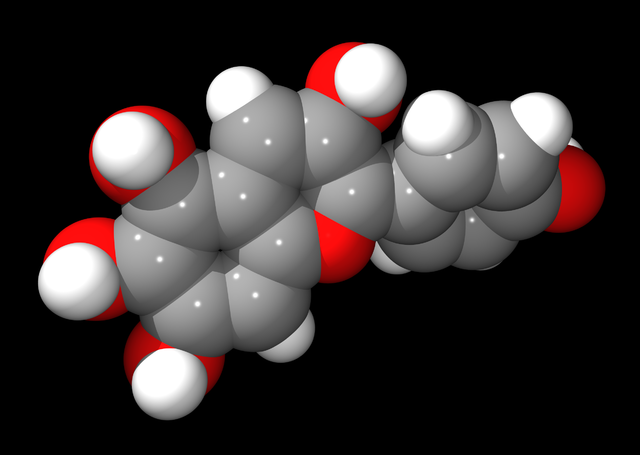
\includegraphics{jmolPart.png}

\bookmarksetup{startatroot}

\chapter{Usando o Jmol para observar moléculas em
3D}\label{usando-o-jmol-para-observar-moluxe9culas-em-3d}

\section{Onde começar ?}\label{onde-comeuxe7ar}

~~~~~~Pode-se começar a usar o \emph{Jmol} de vários modos. Se for usar
em seu computador ou notebook, ou mesmo a partir de uma mídia removível
(\emph{pendrive}), pode acessá-lo baixando, descomprimindo e executando
o arquivo \texttt{Jmol.jar} presente na pasta principal no
\href{https://jmol.sourceforge.net/}{site do Jmol}.

~~~~~~Agora, se não quiser instalar nada, pode também acessá-lo
\emph{online} a partir de diversos sítios. Nesse curso vamos utilizar um
bem famoso, adaptado de um dos próprios desenvolvedores do programa.
Basta clicar nesse
\href{https://chemapps.stolaf.edu/jmol/jmol.php?model=water}{\emph{link}},
numa nova aba, por exemplo:

\begin{Shaded}
\begin{Highlighting}[]
\NormalTok{https}\SpecialCharTok{:}\ErrorTok{//}\NormalTok{chemapps.stolaf.edu}\SpecialCharTok{/}\NormalTok{jmol}\SpecialCharTok{/}\NormalTok{jmol.php?model}\OtherTok{=}\NormalTok{water}
\end{Highlighting}
\end{Shaded}

~~~~~~Agora, clique na molécula com o botão esquerdo do \emph{mouse} ou
com o \emph{touchpad}, e faça movimentos. Ou então gire o botão do meio
do mouse ou realize gestos de afastamento e proximidade com dois dedos
no \emph{touchpad}. A Figura~\ref{fig-telaInicio} que segue ilustra o
resultado.

\begin{figure}

\centering{

\href{https://chemapps.stolaf.edu/jmol/jmol.php?model=water}{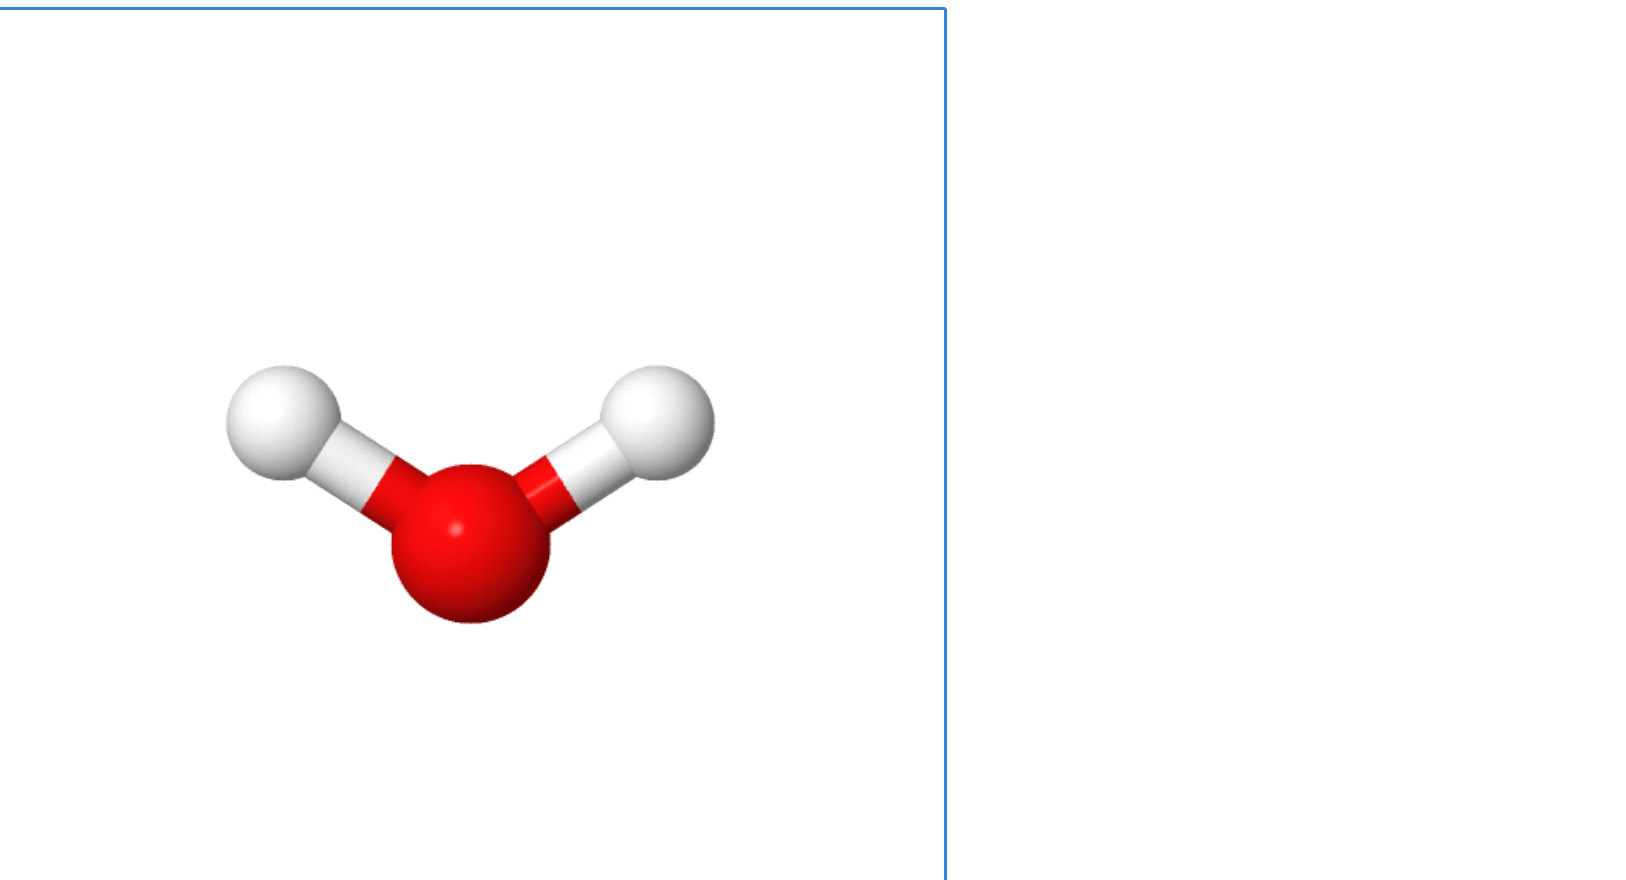
\includegraphics{telaInicio.png}}

}

\caption{\label{fig-telaInicio}Tela (clicável) referente ao modelo da
molécula de água renderizado em navegador pelo \emph{site} do St.~Olaff
College.}

\end{figure}%

~~~~~~Essa é a essência principal ao referenciarmos no título deste
curso a ideia de \textbf{moléculas voadoras}.

\section{\texorpdfstring{Como carregar uma molécula \emph{online}
?}{Como carregar uma molécula online ?}}\label{como-carregar-uma-moluxe9cula-online}

~~~~~~Pra \emph{brincar} um pouco com outra molécula, experimente mudar
o modelo na própria página de internete, ao final da linha. Por exemplo,
de \emph{water} para \emph{tylenol}:

\begin{Shaded}
\begin{Highlighting}[]
\NormalTok{https}\SpecialCharTok{:}\ErrorTok{//}\NormalTok{chemapps.stolaf.edu}\SpecialCharTok{/}\NormalTok{jmol}\SpecialCharTok{/}\NormalTok{jmol.php?model}\OtherTok{=}\NormalTok{tylenol}
\end{Highlighting}
\end{Shaded}

~~~~~~Você pode tentar fazer isso com outras moléculas, digitando seu
nome \emph{em inglês}, por tratar-se de um \emph{site} estrangeiro. Mas
é claro que o banco de dados dessa busca não é ilimitado, e por vezes o
sistema não encontrará a molécula desejada.

~~~~~~Mas há alternativas. Uma delas é buscar o nome da molécula em um
\emph{site} utlizado como banco de dados, o
\href{https://pubchem.ncbi.nlm.nih.gov/}{PubChem}. Exemplificando para a
\emph{vitamina C (ácido ascórbico)}:

\hfill\break

\begin{Shaded}
\begin{Highlighting}[]
\FloatTok{1.}\NormalTok{ Entra no site do [PubChem](https}\SpecialCharTok{:}\ErrorTok{//}\NormalTok{pubchem.ncbi.nlm.nih.gov}\SpecialCharTok{/}\NormalTok{) ;}
\FloatTok{2.}\NormalTok{ Procura por }\StringTok{"ascorbic acid"}\NormalTok{ ;}
\FloatTok{3.}\NormalTok{ Se existir, digite esse mesmo termo ao final da linha do }\SpecialCharTok{*}\NormalTok{JSmol online}\SpecialCharTok{*}\NormalTok{, ou seja}\SpecialCharTok{:}
\NormalTok{    https}\SpecialCharTok{:}\ErrorTok{//}\NormalTok{chemapps.stolaf.edu}\SpecialCharTok{/}\NormalTok{jmol}\SpecialCharTok{/}\NormalTok{jmol.php?model}\OtherTok{=}\NormalTok{ascorbic acid}
\end{Highlighting}
\end{Shaded}

\section{Como baixar uma molécula em seu
computador}\label{como-baixar-uma-moluxe9cula-em-seu-computador}

~~~~~~Caso você digite o nome da molécula no
\href{https://pubchem.ncbi.nlm.nih.gov/}{PubChem} mas não a encontre
após digitar seu nome no \emph{link} do \emph{JSmol} acima, é possível
baixá-la no computador/notebook/tablet/smartphone a partir do
\emph{site} em formato lido pelo \emph{Jmol}. Pra isso, siga os passos
seguintes, exemplificados para o \emph{tetracloreto de carbono}:

\begin{Shaded}
\begin{Highlighting}[]
\FloatTok{1.}\NormalTok{ Entre no site do }\FunctionTok{Pubchem}\NormalTok{ (https}\SpecialCharTok{:}\ErrorTok{//}\NormalTok{pubchem.ncbi.nlm.nih.gov);}
\FloatTok{2.}\NormalTok{ No campo de busca digite }\StringTok{"Carbon Tetrachloride"}\NormalTok{;}
\FloatTok{3.}\NormalTok{ Clique no }\DecValTok{1}\NormalTok{o. composto;}
\FloatTok{4.}\NormalTok{ Clique em }\StringTok{"3D"}\NormalTok{;}
\FloatTok{5.}\NormalTok{ Clique em }\StringTok{"Download coordinates"}\NormalTok{;}
\FloatTok{6.}\NormalTok{ Salve o arquivo clicando na opçao }\StringTok{"Save"}\NormalTok{ para SDF;}
\FloatTok{7.}\NormalTok{ Forneça um nome mais }\StringTok{"amigável"}\NormalTok{ pro arquivo}
\end{Highlighting}
\end{Shaded}

\begin{figure}[H]

{\centering 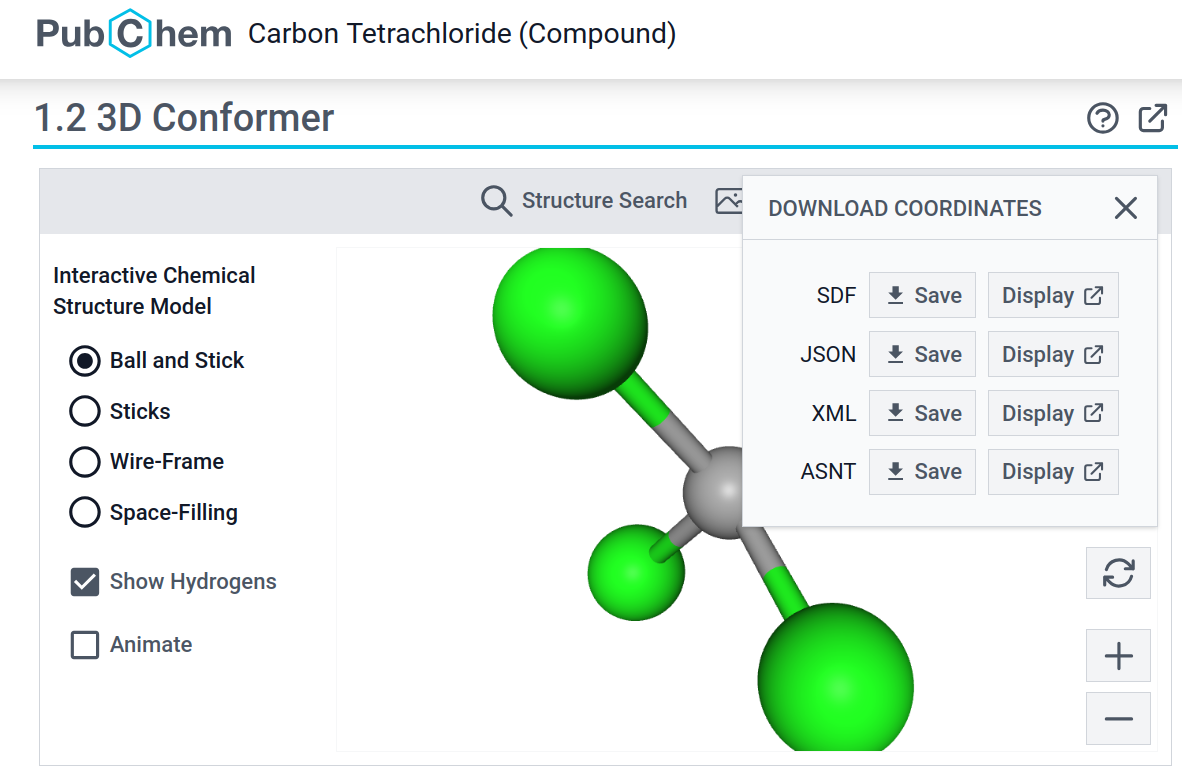
\includegraphics{CCl4.png}

}

\caption{Exemplo para \emph{download} de estrutura molecular no
computador a partir de sua seleção no site \emph{PubChem}.}

\end{figure}%

\section{Como construir a molécula e visualizá-la no
Jmol}\label{como-construir-a-moluxe9cula-e-visualizuxe1-la-no-jmol}

~~~~~~Existem diversos programas de desenho molecular, \emph{online} ou
por instalação, tais como os listados abaixo:

\begin{itemize}
\tightlist
\item
  \href{https://www.acdlabs.com/resources/free-chemistry-software-apps/chemsketch-freeware/}{ChemSketch}
\item
  \href{https://www.rcsb.org/chemical-sketch}{Chemical Sketch Tool}
\item
  \href{https://molview.org/}{MolView}
\item
  \href{https://pubchem.ncbi.nlm.nih.gov//edit3/index.html}{PubChem
  Sketcher}
\item
  \href{https://www.chemdoodle.com/}{ChemDoodle}
\end{itemize}

~~~~~~Também é possível \emph{unir o útil ao (quase)agradável},
carregando uma molécula, adaptando-a ou construindo-a do zero, e
visualizá-la diretamente no \emph{JSmol} ! Para isso recomendamos os
sites abaixo (imagem clicável):

\begin{itemize}
\tightlist
\item
  \href{https://edumol.fi/}{Edumol}.
\end{itemize}

\begin{figure}[H]

{\centering 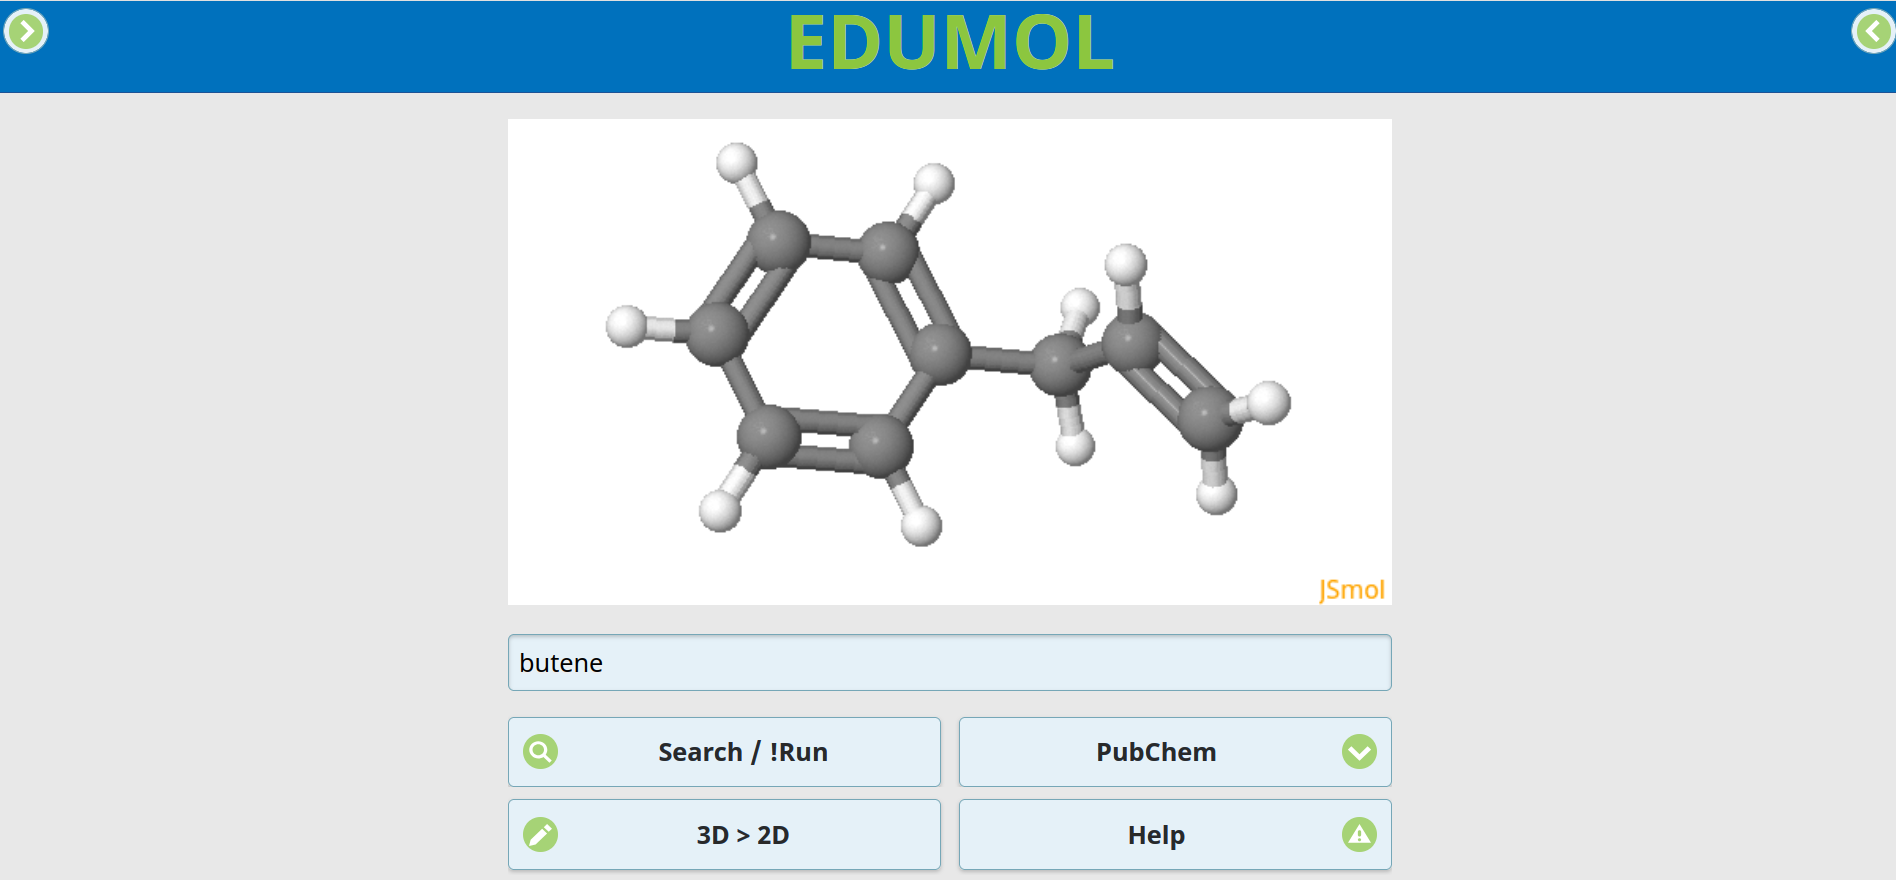
\includegraphics{edumol.png}

}

\caption{Site do \emph{Edumol} para carregamento, modificação e criação
de moléculas renderizáveis em \emph{applet} \emph{JSmol} do próprio
\emph{website}.}

\end{figure}%

\begin{itemize}
\tightlist
\item
  \href{https://chemagic.org/molecules/amini.html}{CheMagic Virtual
  Molecular Model Kit}
\end{itemize}

\begin{figure}[H]

{\centering 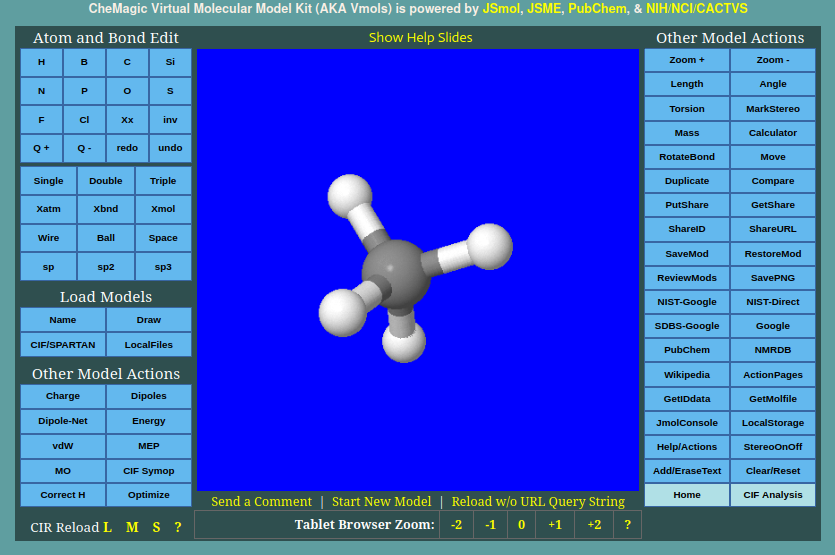
\includegraphics[width=0.8\textwidth,height=\textheight]{chemagic.png}

}

\caption{Site do ChemMagic Virtual Molecular Model Kit, que acessa
diversas funções do \emph{Jmol} por clique de \emph{mouse}.}

\end{figure}%

\bookmarksetup{startatroot}

\chapter{\texorpdfstring{Cliques de mouse \emph{versus} linhas de
comando}{Cliques de mouse versus linhas de comando}}\label{cliques-de-mouse-versus-linhas-de-comando}

\section{Cliques de mouse}\label{cliques-de-mouse}

~~~~~~Qualquer programa de computador que você já tenha usado, ou mesmo
de dispositivos móveis, tem sua \emph{usabilidade} centrada na
facilidade de uso por cliques e arrastes com \emph{mouse},
\emph{touchpad}, e mesmo os dedos (telas capacitivas). Isso facilita
muito as ações rápidas pretendidas. Exemplificando para editores de
texto, é comum se clicar num ícone de formatação (itálico, negrio, por
ex) ou mesmo digitar seu atalho, para concluir o que se deseja no texto.

~~~~~~Simples, prático, e rápido. Dessa mesma forma, pode-se utilizar o
\emph{Jmol}, tanto na versão baixada no computador, como na versão
\emph{online}. Para a versão baixada basta observar a gama de ítens de
menus e submenus. Já para versão de navegador, veja que não há menu !

~~~~~~Não obstante, a versão \emph{online} permite visualizar a mesma
informação, embora com outra formatação, bastando-se clicar \emph{com o
botão direito do mouse} em qualquer área do ecrã (nome chique pra tela
contendo alguma informação, a molécula, no caso).

\section{Linhas de comando}\label{sec-linhasComando}

~~~~~~Assim como para cliques de mouse, também é possível acessar um
campo de texto para digitar comandos do \emph{Jmol}, tanto na versão
baixada (\emph{standalone}), como na versão de navegador (\emph{applet
JSmol}). Para a primeira, clique em \emph{File--\textgreater Console}, e
surgirá uma janela para inserção de texto. Na versão \emph{online},
clique com o botão direito do \emph{mouse} em qualquer ponto do ecrã e
escolha \emph{Console}.

\section{\texorpdfstring{Cliques de mouse \emph{versus} linhas de
comando}{Cliques de mouse versus linhas de comando}}\label{cliques-de-mouse-versus-linhas-de-comando-1}

~~~~~~Ainda que seja possível utilizar o \emph{Jmol} tanto cliques de
mouse como por comandos de texto, qual é o melhor ?

~~~~~~Para auxiliar na resposta, exemplifiquemos com o uso de uma
planilha eletrônica, como o \emph{Excel} do pacote MS-Office, ou o
\emph{Calc} do pacote \emph{Libreoffice}, ou o \emph{Planilhas} da suite
Google. Suponha que você deseje fazer um gráfico simples, pegando duas
colunas, cada qual para uma variável (independente ou \emph{x}, e
dependente, ou \emph{y}). O usual seria clicar em um ítem de menu para
gráficos, selecionar as colunas desejadas em campos específicos da
janela que se abre, selecionar o tipo de gráfico, clicar em
\emph{avançar} ou algum termo similar, selecionar outras características
(etiquetas em \emph{x} e \emph{y}, por ex), e finalmente clicar em
\emph{concluir} (ou \emph{OK}, ou termo de significado similar).
Simples, rápido, e prático.

~~~~~~Mas (sempre tem um ``mas'')\ldots e se você precisasse, além de
construir o gráfico, realizar ações adicionais, como obter o ajuste
linear dos dados, apresentar a reta resultante com determinada cor e
estilo, inserir a equação de reta em um ponto específico do gráfico,
colocar um título, e alterar o símbolo dos pontos, tanto o tipo, quanto
o tamanho e a cor. Ufa !!!

~~~~~~Sem problema, também\ldots desde que você tenha um bom tutorial ao
lado, claro ! Ou que já esteja familiarizado com o programa da planilha,
menus e ações pertinentes aos vários cliques de mouse que serão
necessário para se obter um belo gráfico de regressão linear ao final.

~~~~~~Agora\ldots mais uma pequena variável a inserir ao exemplo
levantado: suponha que não seja você a construir o gráfico, mas um
aluno(a)(a) de sua disciplina, e que não foi treinado nem no uso da
planilha, e nem nos cálculos pretendidos !

~~~~~~Perceba que agora haverá um certo desconforto, posto que:

\begin{enumerate}
\def\labelenumi{\arabic{enumi}.}
\tightlist
\item
  O aluno(a) não possui conhecimento prévio no uso da planilha;
\item
  O aluno(a) não possui conhecimento prévio nos cálculos pretendidos;
\item
  Você terá de treinar o aluno(a), ou oferecer-lhe um \emph{guia} de
  treinamento correlato;
\item
  Caso já tenha ocorrido o treinamento, mas não se esteja com o
  \emph{guia} em mãos, tanto você como aluno(a) dependerão da
  \emph{capacidade de retenção de memória} para efetivar com sucesso a
  empreita.
\end{enumerate}

~~~~~~Agora, e se as orientações para a execução do produto final
estivessem, não num \emph{guia} para a repetição de clique de
\emph{mouse}, mas sim num pequeno texto contendo tanto os comandos em
sequência como os comentários explicativos de cada ação individual, e
que quando inserido no programa gerasse o gráfico todo formatado ?

\section{Vantagens do uso de linhas de comando sobre o uso de
cliques}\label{vantagens-do-uso-de-linhas-de-comando-sobre-o-uso-de-cliques}

~~~~~~Pelo exemplo hipotético acima, perceba que um pequeno texto
contendo as linhas de comando em sequência e os comentários referentes a
esses permitem:

\begin{itemize}
\tightlist
\item
  que o produto final seja elaborado sem prévio conhecimento do
  aluno(a); basta executar o código no programa;
\item
  que o produto final seja elaborado independentemente da memória dos
  envolvidos (sequência de cliques, por ex);
\item
  uma quantidade virtualmente infinita de ações sequenciais, sem
  necessidade de se decorar a ordem dos cliques de \emph{mouse};
\item
  o aprendizado de cada comando utilizado em linguagem humana, posto que
  existem comentários do autor para cada linha;
\item
  que o produto possa ser modificado para gerar um objeto diferente
  (alteração de cor, etiquetas de eixos, outro título, por ex)
\item
  que se reproduza o mesmo gráfico, só que com outros valores para as
  variáveis (\emph{x} e \emph{y});
\item
  que o aprendiz experimente outros comandos para agregar formatações
  e/ou cálculos distintos ao produto;
\item
  que você ou o aluno(a) consigam reproduzir o produto sem recorrer à
  memória e até por séculos depois, se as previsões de extinção em massa
  não vingarem;
\item
  que qualquer pessoa consiga reproduzir o objeto, independentemente de
  seu grau de instrução técnica ou de operabilidade do programa;
\item
  enfim, que se consiga ensinar determinado conteúdo de modo
  reprodutível\ldots ou\ldots{}\textbf{Ensino Reprodutível}.
\end{itemize}

~~~~~~Dessa forma, pretende-se nesse curso utilizar somente \emph{linhas
de comando}, para que se permita materializar-se as vantagens descritas
acima, tangentes a uma metodologia voltada, ainda que incipiente, ao
\emph{Ensino Reprodutível}, e tanto para a ferramenta \emph{Jmol}, como
para a ferramenta \emph{R \& RStudio}.

~~~~~~Em relação ao \emph{Jmol}, portanto, as ações sequenciais para
visualização tridimensional de modelos moleculares será realizada pelo
\emph{Console} acessável conforme ítem Seção~\ref{sec-linhasComando}
acima.

\section{\texorpdfstring{\emph{Scripts}}{Scripts}}\label{scripts}

~~~~~~Colocado da forma acima, quando se tem um conjunto qualquer de
linhas de comando sequenciais, permitindo atuar sobre o modelo molecular
para uma infinidade de coisas, tem-se então um \emph{script}.
Tecnicamente falando, um \emph{script} constitui um bloco de instruções
sequenciais em texto para compilação em um programa.

~~~~~~\emph{Scripts} podem ser elaborados no \emph{Jmol} em
\emph{browser} por duas maneiras:

\begin{Shaded}
\begin{Highlighting}[]
\FloatTok{1.}\NormalTok{ Separando os comandos por }\StringTok{";"} \SpecialCharTok{{-}}\NormalTok{ ex}\SpecialCharTok{:} \StringTok{"cpk only; color blue"}
\FloatTok{2.}\NormalTok{ Separndo os comandos por linhas }\SpecialCharTok{{-}}\NormalTok{ ex}\SpecialCharTok{:}
                                   \StringTok{"cpk only}
\StringTok{                                    color blue"}
\end{Highlighting}
\end{Shaded}

~~~~~~Se você deseja que o modelo realize uns poucos comandos, a melhor
opção é separá-los por ponto e vírgula (``;''). Mas se desejar algo mais
``sofisticado'', sugere-se separá-los por linhas. E mais\ldots linhas
comentadas e escritas em um bloco de notas ou em qualquer editor de
texto !

\subsection{Vantagens do uso de bloco de notas ou editor de texto para
comandos em
série}\label{vantagens-do-uso-de-bloco-de-notas-ou-editor-de-texto-para-comandos-em-suxe9rie}

~~~~~~Imaginando-se uma tranformação mais significativa à molécula
original carregada, como efeitos de ampliação, coloração, representação
e movimento, é fácil perceber que um conjunto de linhas comentadas
dispostas em sequência facilita tanto a observação do que se pretende
com o modelo, como a identificação de erros e ajustes.

~~~~~~Isto também é herdado aos conceitos de \emph{Ensino Reprodutível},
uma vez que facilita a visualização do código (\emph{human readable
format}) e sua depuração (\emph{code debug}). Veja o exemplo que segue,
reflita sobre sua interpretação, copie e teste-o no \emph{Console} do
\emph{Jmol}.

\begin{Shaded}
\begin{Highlighting}[]
\NormalTok{load }\SpecialCharTok{$}\NormalTok{butene}
\NormalTok{background black }\CommentTok{\# cor preta do plano de fundo}
\NormalTok{load }\SpecialCharTok{$}\NormalTok{cholesterol }\CommentTok{\# carrega a molécula de colesterol}
\NormalTok{delay }\DecValTok{1} \CommentTok{\# aguarda 1 segundo}
\NormalTok{background white }\CommentTok{\# altera a cor do plano de fundo}
\NormalTok{spin }\DecValTok{80} \CommentTok{\# gira a molécula}
\NormalTok{delay }\DecValTok{3} \CommentTok{\# ...por 3 segundos}
\NormalTok{spin off }\CommentTok{\# interrompe a rotação}
\NormalTok{cpk }\CommentTok{\# renderiza como modelo de preenchimento}
\NormalTok{color cpk }\CommentTok{\# coloriza no padrão de modelos moleculares}
\NormalTok{isosurface molecular }\CommentTok{\# renderiza a superfície}
\NormalTok{spin }\DecValTok{30} \CommentTok{\# gira mais um poquinho}
\NormalTok{delay }\DecValTok{6} \CommentTok{\# ...também por 3 segundos}
\NormalTok{spin off }\CommentTok{\# interrompe novamente a rotação}
\NormalTok{zoomTo }\FloatTok{0.5} \SpecialCharTok{*}\DecValTok{3}  \CommentTok{\# amplia 300\% na tela durante 1 segundo}
\NormalTok{isosurface off }\CommentTok{\# retira a superfície molecular}
\NormalTok{wireframe only }\CommentTok{\# retorna à representação de varetas}
\NormalTok{wireframe }\DecValTok{50} \CommentTok{\# espessura das varetas}
\NormalTok{zoomTo }\DecValTok{5} \SpecialCharTok{*} \FloatTok{0.01} \CommentTok{\# ... e vai sumindo aos poucos}
\end{Highlighting}
\end{Shaded}

~~~~~~Uma outra opção para adicionar \emph{scripts} diretamente no
\emph{Jmol}, verificar a existência de erros previamente à execução dos
comandos, e testar as linhas passo a passo para a depuração, pode
realizar-se na opção do programa instalado (somente). Para tanto, siga
os passos que seguem.

rode o programa \emph{Jmol} que está no computador ou numa mídia
removível a partir de seu arquivo \emph{Jmol.jar} após descompactação do
arquivo baixado do próprio \href{https://jmol.sourceforge.net/}{site do
\emph{Jmol}}, e escolha do \emph{Script Editor}

\begin{Shaded}
\begin{Highlighting}[]
\FloatTok{1.}\NormalTok{ Entre no site do }\FunctionTok{Jmol}\NormalTok{ (https}\SpecialCharTok{:}\ErrorTok{//}\NormalTok{jmol.sourceforge.net}\SpecialCharTok{/}\NormalTok{) ;}
\FloatTok{2.}\NormalTok{ Faça o Download do programa compactado no computador ou mídia removível ;}
\FloatTok{3.}\NormalTok{ Localize o arquivo compactado que foi baixado ;}
\FloatTok{4.}\NormalTok{ Descompacte o arquivo ;}
\FloatTok{5.}\NormalTok{ Selecione o arquivo }\StringTok{"Jmol.jar"}\NormalTok{, de execução em }\FunctionTok{JAVA}\NormalTok{ (é necessário que o computador tenha a máquina JAVA }\FunctionTok{instalada}\NormalTok{ (JRE), mas isso é comum nos equipamentos com menos de }\DecValTok{10}\NormalTok{ anos }\SpecialCharTok{!!}\NormalTok{)}
\FloatTok{6.}\NormalTok{ Selecione }\StringTok{"File {-}\textgreater{} Script Editor"} 
\end{Highlighting}
\end{Shaded}

~~~~~~Para testar o \emph{Editor de Scripts}, copie e cole o
\emph{script} abaixo para a papaína, uma proteína do mamão:

\begin{Shaded}
\begin{Highlighting}[]
\NormalTok{load}\OtherTok{=}\DecValTok{9}\NormalTok{pap  }\CommentTok{\# carregando a estrutura}
\NormalTok{delay }\DecValTok{2} \CommentTok{\# aguarda 2 segundos}
\NormalTok{cartoon only }\CommentTok{\# representando em desenho}
\NormalTok{color structure }\CommentTok{\# coloração por estrutura 2a.}
\NormalTok{delay }\DecValTok{1} \CommentTok{\# pausa de 1 segundo}
\NormalTok{zoom }\DecValTok{200} \CommentTok{\# ampliação de 2 vezes}
\NormalTok{delay }\DecValTok{1}
\NormalTok{reset }\CommentTok{\# restabelece as coordenadas}
\NormalTok{spin }\DecValTok{300} \CommentTok{\# giro rápido da molécula !}
\end{Highlighting}
\end{Shaded}

~~~~~~Veja que é possível testar se as linhas de comando estão com a
sintaxe correta (\emph{check}), testar os comandos linha a linha
(\emph{step}), ou rodar o \emph{script} como um todo (\emph{run}).

\begin{figure}[H]

{\centering 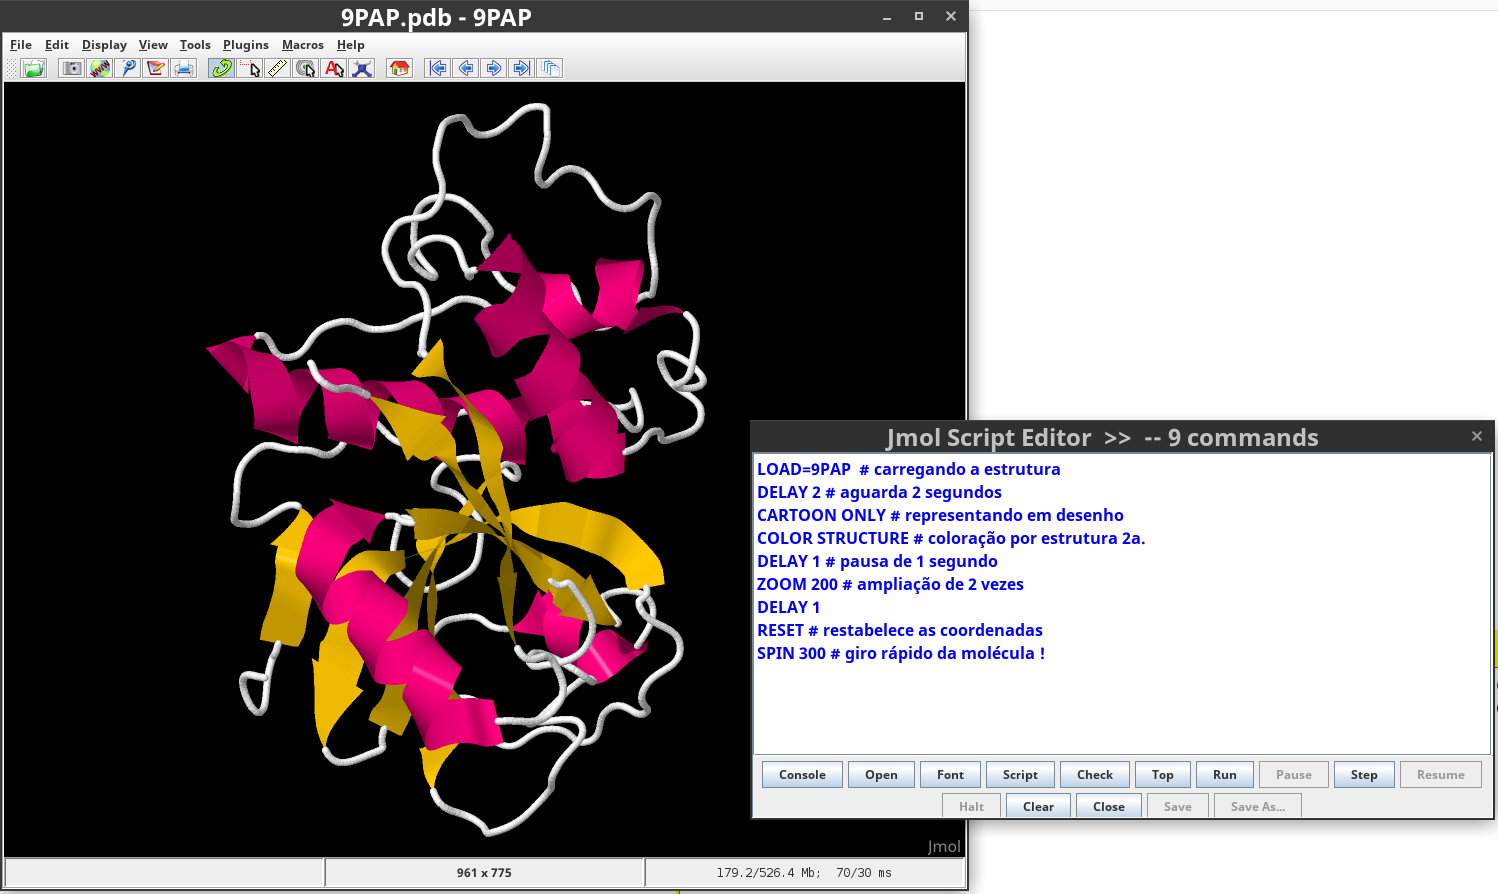
\includegraphics{scriptEditor.png}

}

\caption{Exemplo do uso do \emph{Script Editor} da versão instalada do
\emph{Jmol} em computador ou mídia removível.}

\end{figure}%

~~~~~~Alguns exemplos de \emph{scripts} são ilustrados na
Seção~\ref{sec-selecao}.

\bookmarksetup{startatroot}

\chapter{Alguns comandos pra se aventurar nas moléculas
voadoras}\label{alguns-comandos-pra-se-aventurar-nas-moluxe9culas-voadoras}

\section{Como carregar uma molécula no
JSmol}\label{como-carregar-uma-moluxe9cula-no-jsmol}

~~~~~~Supondo que você já tenha aberto em seu navegador a janela para o
\emph{applet} do \emph{JSmol} mas que, contrariamente ao que foi feito
antes (nome da molécula ao final do \emph{site}
\href{https://pubchem.ncbi.nlm.nih.gov/}{PubChem}, você queira:

\begin{itemize}
\tightlist
\item
  carregar uma molécula a partir de outro banco de dados;
\item
  carregar uma molécula cujo arquivo já esteja em seu computador
\end{itemize}

~~~~~~Bom, nesse caso você pode usar o \emph{mouse} ou uma \emph{linha
de comando}, como preferir.

\subsection{\texorpdfstring{Carregando a molécula com o
\emph{mouse}}{Carregando a molécula com o mouse}}\label{carregando-a-moluxe9cula-com-o-mouse}

~~~~~~Para isto basta clicar com o botão direito do \emph{mouse} no
ecrã, como anteriormente, e selecionar \emph{File--\textgreater Load}.
As opções que se apresentam são:

\begin{Shaded}
\begin{Highlighting}[]
\SpecialCharTok{*}\NormalTok{ Open local file }\CommentTok{\# abre janela para buscar o arquivo do modelo no computador;}
\SpecialCharTok{*}\NormalTok{ Open URL }\CommentTok{\# abre janela para buscar o endereço de internete que possui o arquivo}
\SpecialCharTok{*}\NormalTok{ Get PDB file }\CommentTok{\# abre janela para inserir um código de macromolécula do site homônimo (proteínas, ácidos nucleicos, principalmente)}
\SpecialCharTok{*}\NormalTok{ Get MOL file }\CommentTok{\# abre janela para buscar um arquivo *.mol}
\SpecialCharTok{*}\NormalTok{ Open script }\CommentTok{\# abre janela para buscar um trecho de código no computador}
\end{Highlighting}
\end{Shaded}

~~~~~~A primeira opção é autoexplicativa (\texttt{Open\ local\ file}), a
segunda opção (\texttt{Open\ URL}) depende do endereço correto para um
determinado modelo molecular, a terceira (\texttt{Get\ PDB\ file})
refere-se ao banco de dados \href{https://www.rcsb.org}{Protein Data
Brookhaven} para biopolímeros, a quarta (\texttt{Get\ MOL\ file})
envolve a busca \emph{online} em banco de dados específico para pequenas
moléculas, e a última (\texttt{Open\ script}), a busca de um arquivo que
contenha linhas de código do \emph{Jmol} para um conjunto de ações.

~~~~~~Como os livros didáticos permeiam estruturas moleculares pequenas,
normalmente associadas aos grupos funcionais da \emph{Química Inorgânica
e Orgânica}, bem como exemplos específicos em áreas como \emph{Saúde,
Biotecnologia e Indústria}, incluindo também \emph{alguns modelos de
macromoléculas}, pode-se concluir que é mais provável que você utilize a
busca remota de pequenas moléculas (\emph{Get MOL file}), moléculas
contidas em seu computador (\emph{Open local file}), e/ou
biomacromoléculas (\emph{Get PDB file}).

~~~~~~O carregamento de pequenas moléculas é \emph{idêntico} ao que foi
experimentado adicionando-se o nome do modelo ao final do endereço do
\href{https://chemapps.stolaf.edu/jmol/jmol.php?model=water}{JSmol}. O
carregamento remoto para modelos de proteínas, enzimas e ácidos
nucleicos envolve o conhecimento do \emph{código PDB} desses, ou busca
de palavras-chave no sítio \href{https://www.rcsb.org}{Protein Data
Brookhaven}.

~~~~~~Já o carregamento de moléculas guardadas no PC envolve algumas
poucas etapas, a saber:

\begin{enumerate}
\def\labelenumi{\arabic{enumi}.}
\tightlist
\item
  Obtém-se o modelo da molécula pela internete, ou o constroi;
\item
  Baixa-se o arquivo correspondente ao modelo (geralmente com um
  atributo *.mol, *.cif, *.cml, *.sdf, entre mais de 60 formatos);
\item
  Carrega-se na página do
  \href{https://chemapps.stolaf.edu/jmol/jmol.php?model=water}{JSmol}
  por dois meios alternativos:
\end{enumerate}

\begin{Shaded}
\begin{Highlighting}[]
\FloatTok{1.}\NormalTok{ Por clique de mouse}\SpecialCharTok{:}\NormalTok{ File }\SpecialCharTok{{-}}\OtherTok{{-}\textgreater{}}\NormalTok{ Load }\SpecialCharTok{{-}}\OtherTok{{-}\textgreater{}}\NormalTok{ Open local file ;}
\FloatTok{2.}\NormalTok{ Por arraste do arquivo da pasta onde se encontre para a aba do JSmol no navegador.}
\end{Highlighting}
\end{Shaded}

~~~~Exemplificando, digamos que você queira visualizar a estrutura da
\emph{aspirina} baixada em seu computador.

\begin{Shaded}
\begin{Highlighting}[]
\FloatTok{1.}\NormalTok{ Baixe o modelo estrutural da aspirina em algum site, como o PubChem ;}
\FloatTok{2.}\NormalTok{ Abra o Console do JSmol no }\FunctionTok{navegador}\NormalTok{ (clique no ecrã com o botão direito do mouse e selecione }\StringTok{"Console"}\NormalTok{);}
\FloatTok{3.}\NormalTok{ Alternativamente}\SpecialCharTok{:}
\NormalTok{  a. Localize o arquivo no PC por }\StringTok{"File{-}{-}\textgreater{}Load{-}{-}\textgreater{}Open local file"}\NormalTok{, clicando depois em }\StringTok{"Load"}\NormalTok{ para o carregamento;}
\NormalTok{  b. Clique no arquivo }\FunctionTok{baixado}\NormalTok{ (}\StringTok{"aspirin.sdf"}\NormalTok{, por ex) e arraste}\SpecialCharTok{{-}}\NormalTok{o diretamente para a janela do JSmol. }
\end{Highlighting}
\end{Shaded}

\begin{figure}[H]

{\centering 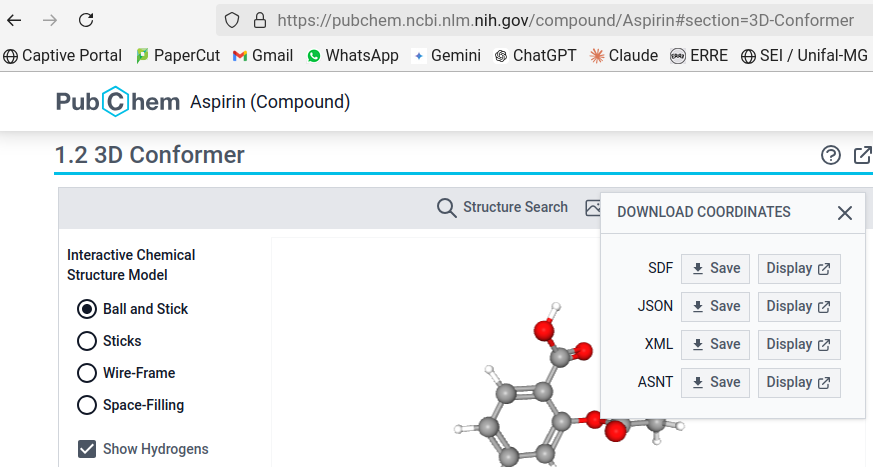
\includegraphics{aspirin.png}

}

\caption{Exemplo do modelo da aspirina para \emph{download} no PubChem.}

\end{figure}%

\subsection{Carregando a molécula por linha de
comando}\label{carregando-a-moluxe9cula-por-linha-de-comando}

~~~~~~O carregamento de um modelo em particular por linha de comando
restringe-se à sua busca pela internete, em banco de dados ou páginas da
\emph{web}. Para isso, abre-se o \emph{Console} como já explicado. A
parte de cima serve para apresentação dos resultados dos comandos, e a
parte de baixo, para sua digitação. Nesse caso, clique no quadro
inferior do \emph{Console} e digite o comando de carregamento, aqui
exemplificado para um \emph{alcano}:

\begin{Shaded}
\begin{Highlighting}[]
\NormalTok{load }\SpecialCharTok{$}\NormalTok{alkane}
\end{Highlighting}
\end{Shaded}

~~~~~~O \emph{Console} do \emph{Jmol}, ainda que constitua uma linguagem
própria de programação de comandos, possui uma vantagem interessante
sobre demais linguagens de programação: \emph{é possível efetuar o
comando pelo Console tanto com letras maiúsculas como minúculas, e tanto
no singular como no plural.}

~~~~~~Você pode tentar com outras moléculas, como \emph{aspirin},
\emph{cholesterol}, \emph{phenol} etc (nomes em inglês, por conta do
banco de dados). Para recuperar uma linha de comando que foi escrita
antes, basta navegar entre os comandos que foram utilizados com as setas
para cima e para baixo do teclado.

Os modelos moleculares são carregados a partir do banco de dados
\href{https://cactus.nci.nih.gov/chemical/structure}{Cactus - CADD Group
Chemoinformatics Tools and User Services}.

\subsubsection{Carregando moléculas por notação
SMILES}\label{carregando-moluxe9culas-por-notauxe7uxe3o-smiles}

~~~~~~\href{https://pt.wikipedia.org/wiki/SMILES}{SMILES-Simplified
Molecular Input Line Entry System} trata de uma notação química que
permite representar as moléculas inserindo-se o nome de cada átomo em
sequência em ligações simples, bem como o local de ligações insaturadas,
ou ligações aromáticas.

~~~~~~O \href{https://pubchem.ncbi.nlm.nih.gov/}{PubChem} possui também
a notação \emph{SMILES} como alternativa para carregamento de modelos.
Seguem alguns exemplos da notação para carregamento da molécula no
\emph{Console} do \emph{Jmol}.

~~~~~~Para hidrocarbonetos sem ligações insaturadas (\emph{alcanos}) é
possível carregar a molécula digitando somente a sequência de carbonos,
como segue:

\begin{Shaded}
\begin{Highlighting}[]
\CommentTok{\# Para carregar um metano}
\NormalTok{load }\SpecialCharTok{$}\NormalTok{C }\CommentTok{\# carrega o modelo}
\end{Highlighting}
\end{Shaded}

\begin{Shaded}
\begin{Highlighting}[]
\CommentTok{\# Para carregar um hexano}
\NormalTok{load }\SpecialCharTok{$}\NormalTok{CCCCCC }\CommentTok{\# carrega o modelo}
\end{Highlighting}
\end{Shaded}

~~~~~~Agora, para carregar hidrocarbonetos com uma ligação insaturada
(\emph{alcenos}), basta inserir o sinal de igualdade (\emph{=}) onde
aparece a insaturação:

\begin{Shaded}
\begin{Highlighting}[]
\CommentTok{\# Para carregar um propeno (propileno)}
\NormalTok{load }\SpecialCharTok{$}\NormalTok{CC}\OtherTok{=}\NormalTok{C }\CommentTok{\# carrega o modelo}
\end{Highlighting}
\end{Shaded}

~~~~~~Para carregar um modelo com ligação tripla, segue-se a notação
\emph{\#}:

\begin{Shaded}
\begin{Highlighting}[]
\CommentTok{\# Para carregar um metilacetileno (ou ....propina !)}
\NormalTok{load }\SpecialCharTok{$}\NormalTok{CC}\CommentTok{\#C \# carrega o modelo}
\end{Highlighting}
\end{Shaded}

~~~~~~Para carregar uma estrutura aromática, já um pouco mais chatinho:

\begin{Shaded}
\begin{Highlighting}[]
\CommentTok{\# Para carregar um benzeno}
\NormalTok{load }\SpecialCharTok{$}\NormalTok{C1}\OtherTok{=}\NormalTok{CC}\OtherTok{=}\NormalTok{CC}\OtherTok{=}\NormalTok{C1 }
\end{Highlighting}
\end{Shaded}

\subsection{Carregando biopolímeros (proteínas, enzimas, ácidos
nucleicos) por linha de
comando}\label{carregando-biopoluxedmeros-proteuxednas-enzimas-uxe1cidos-nucleicos-por-linha-de-comando}

~~~~~~Como mecionado acima, o carregamento de macromoléculas biológicas
dá-se por identificação de um código alfanumérico da mesma frente ao
banco de dados \href{https://www.rcsb.org/}{PDB-Protein Data Bank}. Após
obter esse código, o comando de carregamento é:

\begin{Shaded}
\begin{Highlighting}[]
\NormalTok{load}\OtherTok{=}\NormalTok{XXXX }\CommentTok{\# onde XXXX é o código da macromolécula110}
\CommentTok{\# Obs: Perceba que o sinal de "$" é trocado por "=" para o PDB}
\end{Highlighting}
\end{Shaded}

~~~~~~Isso pode ser ilustrado por carregamento remoto da proteína
espícula (\emph{spike}) do vírus Sars-Cov-2, tal como segue:

\begin{Shaded}
\begin{Highlighting}[]
\FloatTok{1.}\NormalTok{ Entre no site do PDB}\SpecialCharTok{{-}}\NormalTok{Protein Data Bank }\SpecialCharTok{{-}}\NormalTok{ https}\SpecialCharTok{:}\ErrorTok{//}\NormalTok{www.rcsb.org}\SpecialCharTok{/}\NormalTok{ ; }
\FloatTok{2.}\NormalTok{ No campo de busca, digite }\StringTok{"spike sars{-}cov{-}2"}\NormalTok{ ;}
\FloatTok{3.}\NormalTok{ Selecione a }\DecValTok{1}\NormalTok{a opção (o site vai direcionar para várias estruturas da proteína espícula) ;}
\FloatTok{4.}\NormalTok{ Memorize o código da }\DecValTok{1}\NormalTok{a. opção (embora qualquer uma também sirva), ou seja, }\StringTok{"7FCD"}\NormalTok{ ;}
\FloatTok{5.}\NormalTok{ Digite a linha para carregar a proteína}\SpecialCharTok{:} \StringTok{"load=7FCD"}\NormalTok{ (tanto faz se maiúsculas ou minúsculas)}
\end{Highlighting}
\end{Shaded}

~~~~~~A representação padrão para proteínas no \emph{Jmol} é a de arame
(\emph{wireframe}). Para visualizar a proteína do vírus de modo mais
``amigável'' e semelhante ao que aparece em textos ou na internete,
digite os comandos abaixo.

\begin{Shaded}
\begin{Highlighting}[]
\NormalTok{cartoon only  }\CommentTok{\# representação exclusiva de desenho da estrutura de biopolímeros}
\NormalTok{color chain }\CommentTok{\#  coloração por "cadeias" da proteína}
\end{Highlighting}
\end{Shaded}

\begin{figure}[H]

{\centering 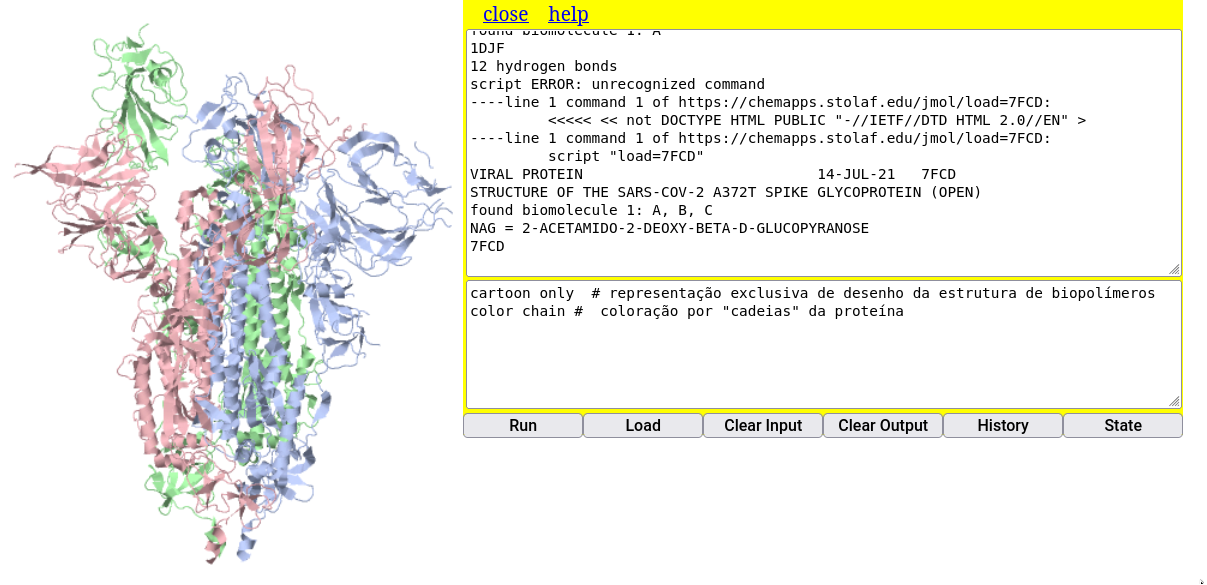
\includegraphics{spike.png}

}

\caption{Representação da proteína \emph{spike} do vírus de Sars-Cov-2
(coloração por número de cadeias.}

\end{figure}%

~~~~~~Proteínas, enzimas, ácidos nucleicos, e associações
macromoleculares são mais pertinentes ao estudo da \emph{Bioquímica}
estrutural. Nesse sentido lhe convido a visitar uma parte do
\emph{website} autoral que possui descrições e representações detalhadas
de estruturas bioquímicas com auxílio do \emph{Jmol}, o site
\href{https://bioquanti.netlify.app/}{Bioquanti}

\begin{figure}[H]

{\centering 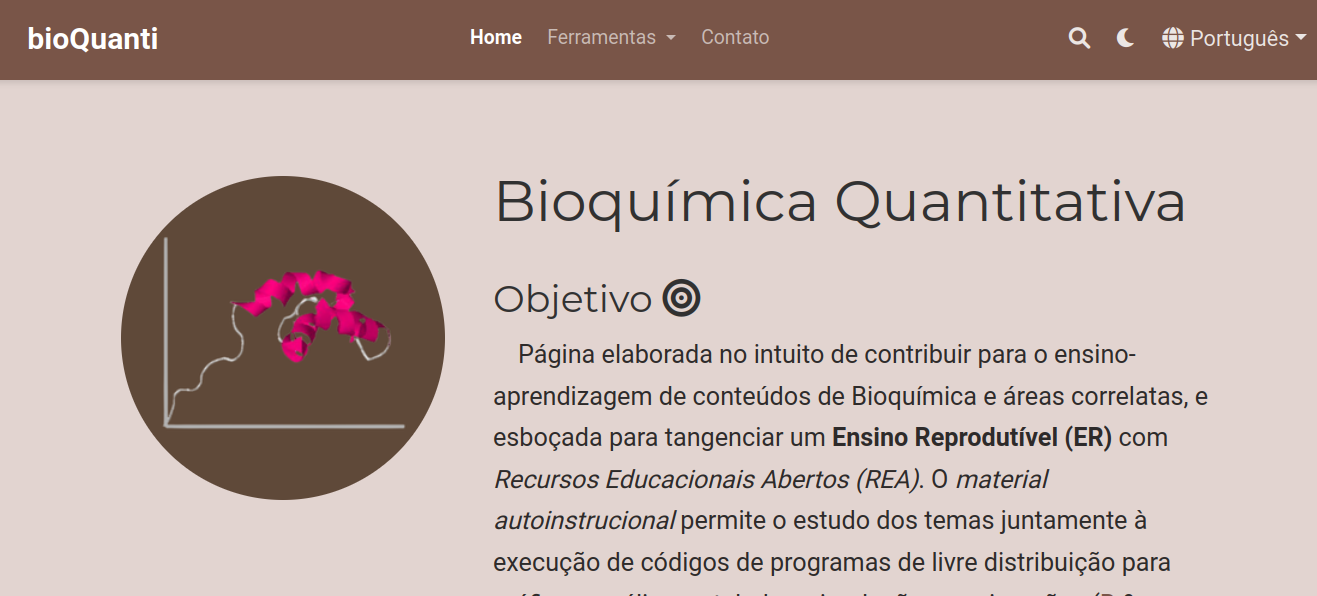
\includegraphics{bioquanti.png}

}

\caption{Bioquanti, um website autoral para estudos quantitativos em
Bioquímica, e que inclui diversos modelos moleculares para o
\emph{Jmol}.}

\end{figure}%

\section{Agora que a molécula está na página do navegador, o que posso
fazer com ela
?}\label{agora-que-a-moluxe9cula-estuxe1-na-puxe1gina-do-navegador-o-que-posso-fazer-com-ela}

~~~~~~Muuuuuiiita coisa !!!

~~~~~~O \emph{Jmol} possui um \emph{menu} com diversas operações, e
centenas de comandos, e talvez outra centena de tutoriais pela
internete. Para observações estruturais mais diretas e imediatas,
contudo, pode-se resumir as operações em:

\begin{itemize}
\tightlist
\item
  Movimentos com mouse (rotação, translação, \emph{zoom})
\item
  Representações do modelo (bola e varetas, espaço preenchido, arame)
\item
  Cores (modelo e plano de fundo)
\item
  Medidas (distâncias e ângulos)
\item
  Características moleculares (ligações de H, nuvem de van der Waals,
  carga parcial e efetiva)
\item
  Superfícies (molecular, eletrostática)
\item
  Seleção de átomos e visualização (água, hidrogênio)
\item
  Animações (zoom, rotação automática), cortes
\end{itemize}

~~~~~~Uma observação importante é que \emph{todos dos comandos do Jmol
possuem ajuda explicativa}. Para tanto, basta digitar:

\begin{Shaded}
\begin{Highlighting}[]
\NormalTok{help nome.do.comando}
\end{Highlighting}
\end{Shaded}

\section{Salvamento do modelo no computador ou dispositivo
móvel}\label{salvamento-do-modelo-no-computador-ou-dispositivo-muxf3vel}

~~~~~~Todas as ações realizadas com a molécula produzem um novo modelo
que pode ser baixado para o computador. E isso é bem legal porque a
molécula modificada (com alteração de cores, representações, animações,
por ex) pode ser carregada no \emph{Jmol} ou na \emph{JSmol} (internet)
como já mencionado. Para tanto, pode-se usar cliques de mouse ou linhas
de comando, como segue:

\begin{Shaded}
\begin{Highlighting}[]
\FloatTok{1.}\NormalTok{ Botão direito no ecrã }\OtherTok{{-}\textgreater{}}\NormalTok{ File }\OtherTok{{-}\textgreater{}}\NormalTok{ Save }\OtherTok{{-}\textgreater{}}\NormalTok{ Save as PNG}\SpecialCharTok{/}\NormalTok{JMOL }\CommentTok{\# por mouse}
\FloatTok{2.}\NormalTok{ write nome\_da\_molecula }\CommentTok{\# por linha de comando no Console}
\end{Highlighting}
\end{Shaded}

Obs: a opção PNG/JMOL é muito interessante, já que permite visualizar o
modelo trabalhado em qualquer editor de imagem, bem como no \emph{Jmol}.

~~~~~~Para exemplificar essas ações, usaremos inicialmente o modelo da
\emph{vitamina C}, carregando-o com o comando
\texttt{load\ \$ascorbate}. Mas se você quiser saber todos os comandos
possíveis, faça uma visita ao
\href{https://chemapps.stolaf.edu/jmol/docs/}{\emph{site} de referência
do \emph{Jmol}}.

\section{Movimentos com mouse}\label{movimentos-com-mouse}

~~~~~~Para rotação e translação do modelo, bem como ampliação:

\begin{Shaded}
\begin{Highlighting}[]
\NormalTok{zoom }\SpecialCharTok{{-}}\NormalTok{ botão do meio do mouse; se não houver o botão, Shift}\SpecialCharTok{+}\NormalTok{botão esquerdo}
\NormalTok{rotação }\SpecialCharTok{{-}}\NormalTok{ botão esquerdo do mouse}
\NormalTok{translação }\SpecialCharTok{{-}}\NormalTok{ Ctrl}\SpecialCharTok{+}\NormalTok{botão direito}
\NormalTok{rotação no eixo }\SpecialCharTok{{-}}\NormalTok{ Shift}\SpecialCharTok{+}\NormalTok{botão direito}
\end{Highlighting}
\end{Shaded}

\section{Representações do modelo}\label{representauxe7uxf5es-do-modelo}

~~~~~~As representações referem-se ao aspecto visual do modelo
(renderização). Assim, o \emph{Jmol} pode renderizar o modelo como
v\emph{areta, arame, espaço preenchido, bola e vareta, traço, e
desenho}. Experimente renderizar o nesses tipos, incluindo a opção
\texttt{only}. Essa opção permite que a ação não seja sobreposta às
anteriores (no caso, a sobreposição das representações).

\begin{Shaded}
\begin{Highlighting}[]
\NormalTok{wireframe only }\CommentTok{\# arame}
\NormalTok{cpk only }\CommentTok{\# espaço preenchido}
\NormalTok{trace only }\CommentTok{\# traço}
\NormalTok{cartoon only }\CommentTok{\# desenho}
\end{Highlighting}
\end{Shaded}

~~~~~~Observe também que representação em \texttt{cartoon} não resulta
numa renderização para o modelo da vitamina C. Isso decorre porque a
representação em \texttt{cartoon} é restrita para biopolímeros, ou seja,
proteínas e ácidos nucleicos.

~~~~~~Contudo, se quiser experimentar o \texttt{cartoon}, será
necessário conhecer o código alfanumérico de uma proteína ou ácido
nucleico. Exemplificando para a mioglobina, proteína transportadora de
oxigênio em mamíferos (código: \emph{1mcy})

\begin{Shaded}
\begin{Highlighting}[]
\NormalTok{load}\OtherTok{=}\DecValTok{1}\NormalTok{mcy }\CommentTok{\# carregando a mioglobina}
\end{Highlighting}
\end{Shaded}

~~~~~~Veja que a renderização padrão para grandes moléculas é a de bolas
e varetas, pouco didática para o aprendiz. Nesse caso, pode-se
representá-la como desenho exclusivo, digitando-se:

\begin{Shaded}
\begin{Highlighting}[]
\NormalTok{cartoon only }\CommentTok{\# renderizando em desenho}
\end{Highlighting}
\end{Shaded}

~~~~~~Para se conseguir esse e outros códigos de proteínas e ácidos
nucleicos, deve-se entrar no banco de dados do
\href{https://www.rcsb.org/}{PDB - Protein Data Bank, RCSB}, e digitar o
nome no campo de busca (no caso, \texttt{myoglobin}). O sistema retorna
diversos modelos estruturais e seus códigos, bastando transcrever um
desses códigos ao \emph{Console} do \emph{JSmol}.

\section{Cores}\label{cores}

~~~~~~Existe grande flexibilidade de
\href{https://jmol.sourceforge.net/jscolors/}{cores} para o \emph{Jmol}
(e, por consequência, para o \emph{JSmol}), tanto para os modelos
inteiros, partes do modelo (átomos específicos ou um conjunto), e plano
de fundo. A visualização padrão de cores segue a convenção
\href{https://en.wikipedia.org/wiki/CPK_coloring}{CPK
(Corey--Pauling--Koltun)}. Exemplificando para o modelo anterior de
vitamina C (\texttt{load\ \$ascorbate}), experimente a variação que
segue:

\begin{Shaded}
\begin{Highlighting}[]
\NormalTok{color pink}
\NormalTok{color blue}
\NormalTok{color ligthgreen}
\NormalTok{background yellow }\CommentTok{\# plano de fundo}
\end{Highlighting}
\end{Shaded}

~~~~~~O último comando da lista acima permite variar a coloração do
plano de fundo.

~~~~~~Adicionalmente, também é possível a coloração de ligações entre os
átomos, como segue:

\begin{Shaded}
\begin{Highlighting}[]
\NormalTok{color bonds LightSeaGreen}
\end{Highlighting}
\end{Shaded}

~~~~~~Para um grande espectro de cores, você pode consultar a referência
do \href{https://jmol.sourceforge.net/jscolors/}{Jmol Colors}, ou um
\emph{link} mais ``mastigado'', de nossa autoria junto ao aprendizado do
programa no ensino superior, o portal
\href{https://bioquanti.netlify.app/}{Bioquanti} e, mais
especificamente, o
\href{https://bioquanti.netlify.app/uploads/jmolbook/jmolquarto/comandos\#cores-espec\%C3\%ADficas}{tópico
de cores para o Jmol}.

\section{Medidas}\label{medidas}

~~~~~~O \emph{Jmol} permite calcular distâncias e ângulos em um modelo
molecular. Para exemplificar isso, talvez seja interessante o
carregamento de um \emph{modelo de água} (\texttt{load\ \$water}), e
cujas distâncias e ângulos estão presentes em alguns livros de Química.

\subsection{Para distâncias}\label{para-distuxe2ncias}

~~~~~~No exemplo da molécula de água, para se determinar a distância de
uma ligação O-H, por exemplo:

\begin{Shaded}
\begin{Highlighting}[]
\FloatTok{1.}\NormalTok{ Duplo}\SpecialCharTok{{-}}\NormalTok{clique do mouse no }\DecValTok{1}\NormalTok{o. átomo;}
\FloatTok{2.}\NormalTok{ Arraste do mouse ao }\DecValTok{2}\NormalTok{o. átomo;}
\FloatTok{3.}\NormalTok{ Clique do mouse no }\DecValTok{2}\NormalTok{o. átomo}
\end{Highlighting}
\end{Shaded}

~~~~~~Experimentando para a distância da ligação O-H, o programa retorna
o valor de 0,097 nm, ou 0,97 Angstroms, o valor convencial para esse
tipo de ligação covalente.

\begin{figure}[H]

{\centering 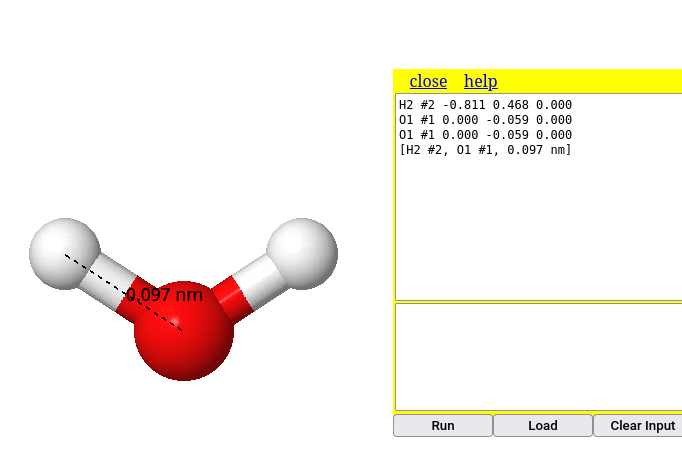
\includegraphics{aguaDist.png}

}

\caption{Medindo distância dentro da molécula.}

\end{figure}%

\subsection{Para ângulos}\label{para-uxe2ngulos}

~~~~~~Para a mesma molécula de água, experimente determinar o ângulo de
ligação:

\begin{Shaded}
\begin{Highlighting}[]
\FloatTok{1.}\NormalTok{ Duplo clique no }\DecValTok{1}\NormalTok{o. á}\FunctionTok{tomo}\NormalTok{ (ex}\SpecialCharTok{:}\NormalTok{ H);}
\FloatTok{2.}\NormalTok{ Arrasta ao }\DecValTok{2}\NormalTok{o. á}\FunctionTok{tomo}\NormalTok{ (ex}\SpecialCharTok{:}\NormalTok{ O);}
\FloatTok{3.}\NormalTok{ Clique no }\DecValTok{2}\NormalTok{o. átomo;}
\FloatTok{4.}\NormalTok{ Arraste ao }\DecValTok{3}\NormalTok{o. á}\FunctionTok{tomo}\NormalTok{ (ex}\SpecialCharTok{:}\NormalTok{ o outro H);}
\FloatTok{5.}\NormalTok{ Clique no }\DecValTok{3}\NormalTok{o. átomo}
\end{Highlighting}
\end{Shaded}

~~~~~~Perceba que o sistema retorna o valor de 114\(^{o}\), um valor
próximo do previsto para a molécula (109.5\(^{o}\)), ou medido
(104.5\(^{o}\)). Essa aproximação é decorrente da construção do modelo
de água.

\begin{figure}[H]

{\centering 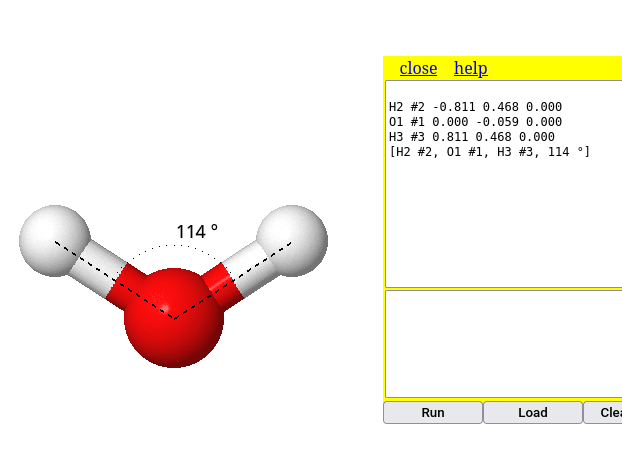
\includegraphics{aguaAng.png}

}

\caption{Medindo ângulo dentro da molécula.}

\end{figure}%

~~~~~~Para limpar as medidas, use o comando:

\begin{Shaded}
\begin{Highlighting}[]
\NormalTok{measure off}
\end{Highlighting}
\end{Shaded}

\section{Características
moleculares}\label{caracteruxedsticas-moleculares}

~~~~~~São diveras as informações tangíveis a um modelo molecular no
\emph{Jmol}. Exemplificando as mais básicas para a molécula de um
componente do molho \emph{shoyo}, o glutamato:

\subsection{Cargas}\label{cargas}

~~~~~~Há dois tipos de cargas oferecidas pelo \emph{Jmol}, \emph{carga
efetiva (\texttt{formaCharge}) e carga parcial
(\texttt{partialcharge})}. Exemplificando, digite no \emph{Console} os
comandos abaixo:

\begin{Shaded}
\begin{Highlighting}[]
\NormalTok{calculate partialCharges }\CommentTok{\# cálculo de cargas parciais do modelo}
\NormalTok{label \%P }\CommentTok{\# apresentação das cargas (etiquetagem)}
\end{Highlighting}
\end{Shaded}

~~~~~~Uma característica do \emph{Jmol} que o torna mais eficiente a
execução de suas ações é a disposição sequencial de comandos. Dessa
forma, não é necessário clicar em \emph{Enter} para cada comando,
bastando separar os comando por ponto e vírgula (\emph{;}) como
ilustrado abaixo:

\begin{figure}[H]

{\centering 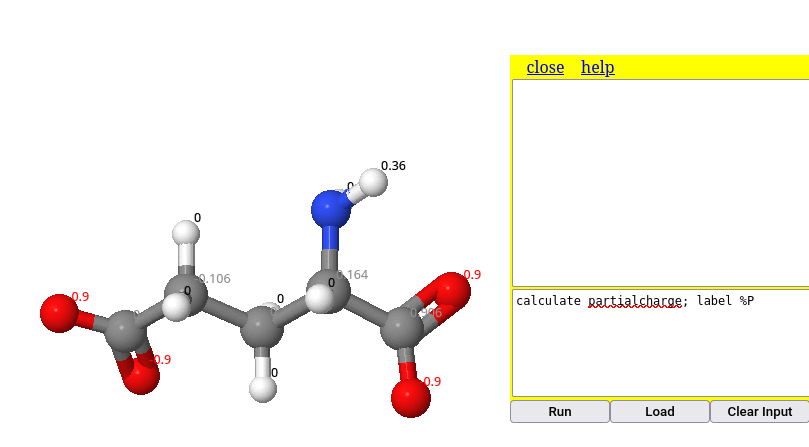
\includegraphics{glu.png}

}

\caption{Aprentação de cargas parciais no modelo de glutamato, um
componente do molho Shoyo, também ilustrando uma sequência de ações no
Jmol.}

\end{figure}%

~~~~~~Da mesma forma pode-se ilutrar a obtenção de \emph{cargas formais}
no modelo. Nessa, adicionou-se a coloração transparente, para melhor
visualização da carga unitária negativa do ácido carboxílico:

\begin{Shaded}
\begin{Highlighting}[]
\NormalTok{calculate formalcharges }\CommentTok{\# cálculo de cargas parciais do modelo}
\NormalTok{label \%C }\CommentTok{\# apresentação das cargas (etiquetagem)}
\end{Highlighting}
\end{Shaded}

\begin{figure}[H]

{\centering 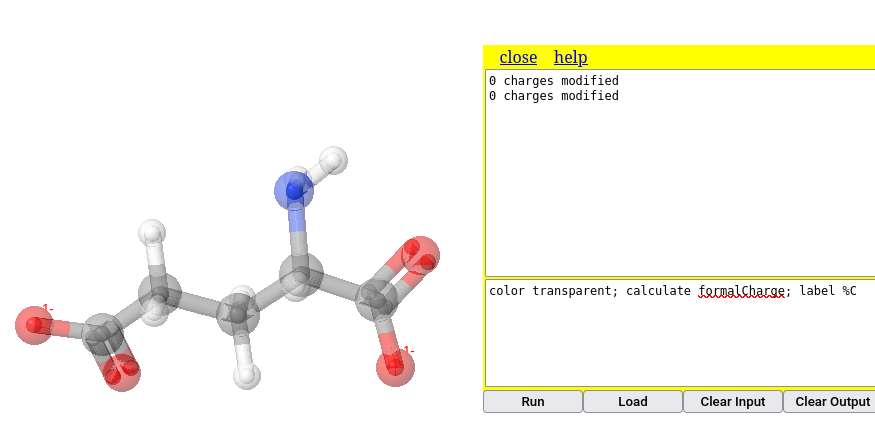
\includegraphics{gluFormal.png}

}

\caption{Ilustração dos comandos em sequência para visualização de
cargas formais na molécula de glutamato.}

\end{figure}%

~~~~~~Perceba que os comando da figura mistura maiúscula e minúsculas,
de modo diferente da linha de comando que a antecede. Essa é uma
\textbf{característica bem legal do \emph{Jmol}, que não se importa com
a capitalização ou não da fonte}. Ou seja, tanto faz se minúsculo,
maiúsculo ou uma combinação de ambos; o \emph{Jmol} executa a ação do
mesmo modo.

\subsubsection{Scripts \& Ensino
Reprodutível}\label{scripts-ensino-reprodutuxedvel}

~~~~~~O exemplo acima apresenta uma maneira simples de concatenar
comandos, facilitando a execução automático e sequencial de um conjunto
desses. No entanto, a visualização da linha de comando fica um pouco
prejudicada com a separação por \emph{``;''}, o que pode acarretar uma
poluição visual quando houver vários comandos.

~~~~~~A situação de contorno envolve a disposição dos comandos no
formato de um \emph{script}. Esse nada mais é do que um trecho de código
contendo um comando por linha, o que melhora a visualização do código
como um todo. Além disso, o \emph{script} possui a vantagem adicional de
se inserir comentários entre as linhas de comando, permitindo também uma
melhor apropriação do código e de seu aprendizado.

~~~~~~Essas características de um \emph{comando por linha com
comentários explicativos} conferem ao \emph{Jmol} seu aspecto para
\emph{programação} de ações sequenciais, e enraiza por consequência uma
das premissas básicas para um \emph{Ensino Reprodutível}: a redação de
trechos de códigos em comandos unitários por linha, escritos como num
bloco de notas, e com comentários sobre as ações do programa em cada
linha. Exemplificando para um \emph{script} envolvendo as ações para o
glutamato acima, apenas copie o trecho abaixo e cole-o no \emph{Console}
do \emph{JSmol}, executando-o.

\begin{Shaded}
\begin{Highlighting}[]
\NormalTok{load }\SpecialCharTok{$}\NormalTok{glu }\CommentTok{\# carregamento de micromolécula }
\NormalTok{wireframe only }\CommentTok{\# renderização exclusiva de varetas}
\NormalTok{calculate partialCharge }\CommentTok{\# carga parcial}
\NormalTok{label \%P }
\end{Highlighting}
\end{Shaded}

~~~~~~Outro aspecto inerente à iniciativa de \emph{Ensino Reprodutível}
reside na \emph{possibilidade de se avaliar o código com alguma
alteração}, objetivando um produto final ligeiramente modificado. Tente
repetir o trecho acima, mas para cargas efetivas, ou seja:

\begin{Shaded}
\begin{Highlighting}[]
\NormalTok{load }\SpecialCharTok{$}\NormalTok{glu }\CommentTok{\# carregamento de micromolécula }
\NormalTok{cpk only }\CommentTok{\# renderização exclusiva por espaço preenchido}
\NormalTok{calculate formalCharge }\CommentTok{\# carga efetiva }
\NormalTok{label \%C }
\end{Highlighting}
\end{Shaded}

~~~~~~Complementarmente, pode-se atuar alterando mais comandos do
código, de modo a criar um resultado completamente diferente do
original. Isso define outra característica do \emph{Ensino
Reprodutível}, qual seja, a de \emph{criação de trecho de código}.
Ilustrando, segue um trecho baseado no anterior, mas para minimização de
energia e reestruturação dos orbitais da molécula.

\begin{Shaded}
\begin{Highlighting}[]
\NormalTok{load }\SpecialCharTok{$}\NormalTok{glu }\CommentTok{\# carregamento de micromolécula }
\NormalTok{cpk only }\CommentTok{\# renderização exclusiva por espaço preenchido}
\NormalTok{minimize }\CommentTok{\# comando para minimização de energia da estrutura }
\end{Highlighting}
\end{Shaded}

\section{Características
moleculares}\label{caracteruxedsticas-moleculares-1}

~~~~~~Além de previsão estrutural para \emph{carga parcial e carga
formal} (embora essa última dependa na prática de informação adicional,
o valor de pH do meio), o \emph{Jmol} também permite evidenciar
\emph{forças fracas} no modelo, tais como \emph{nuvem de van der Waals}
e \emph{ligações de hidrogênio}, como segue.

\subsection{Nuvem de van der Waals}\label{nuvem-de-van-der-waals}

\begin{Shaded}
\begin{Highlighting}[]
\NormalTok{dots on }\CommentTok{\# nuvem de van der Waals nos átomos do modelo (retira{-}se com "dots off")}
\NormalTok{calculate hbonds }\CommentTok{\# identifica ligações de hidrogênio no modelo}
\end{Highlighting}
\end{Shaded}

~~~~~~Ilustrando, copie e cole o trecho que segue no \emph{Console}:

\begin{Shaded}
\begin{Highlighting}[]
\NormalTok{load }\SpecialCharTok{$}\NormalTok{water}
\NormalTok{dots on }\CommentTok{\# nuvem de van der Waals na estrutura da água}
\NormalTok{dots ionic }\CommentTok{\# nuvem iônica sobre o modelo}
\end{Highlighting}
\end{Shaded}

\begin{figure}[H]

{\centering 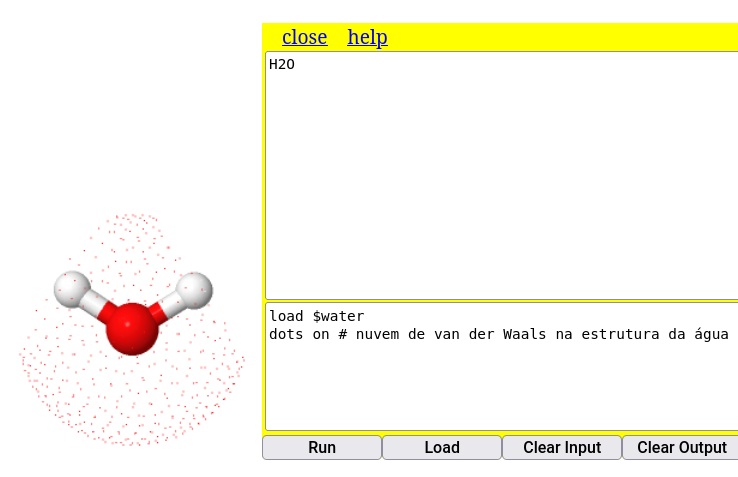
\includegraphics{vanderwaals.png}

}

\caption{Exemplificando a sobreposição de nuvens de van der Waals nos
átomos da molécula de água.}

\end{figure}%

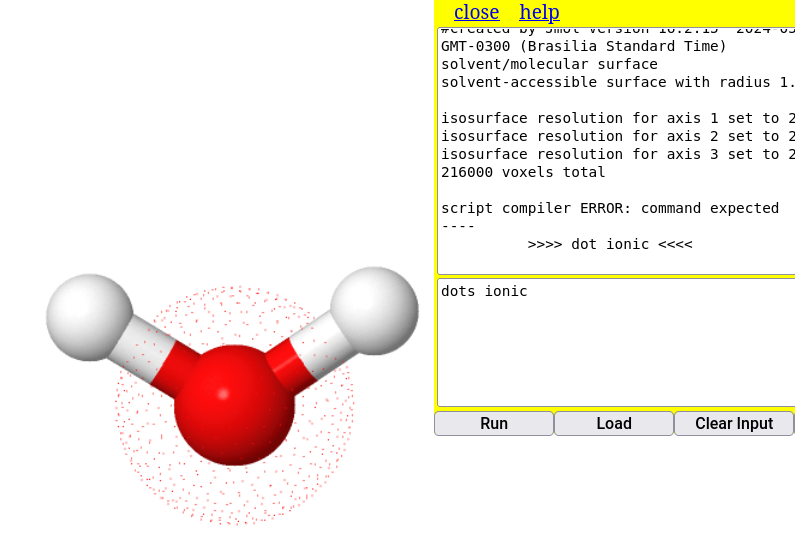
\includegraphics{ionic.png} \#\#\# Ligações de hidrogênio

\begin{Shaded}
\begin{Highlighting}[]
\NormalTok{load}\OtherTok{=}\DecValTok{1}\NormalTok{djf }\CommentTok{\# carrega um modelo de peptídio}
\NormalTok{calculate hbonds }\CommentTok{\# apresenta as ligações de H presentes na estrutura}
\end{Highlighting}
\end{Shaded}

\begin{figure}[H]

{\centering 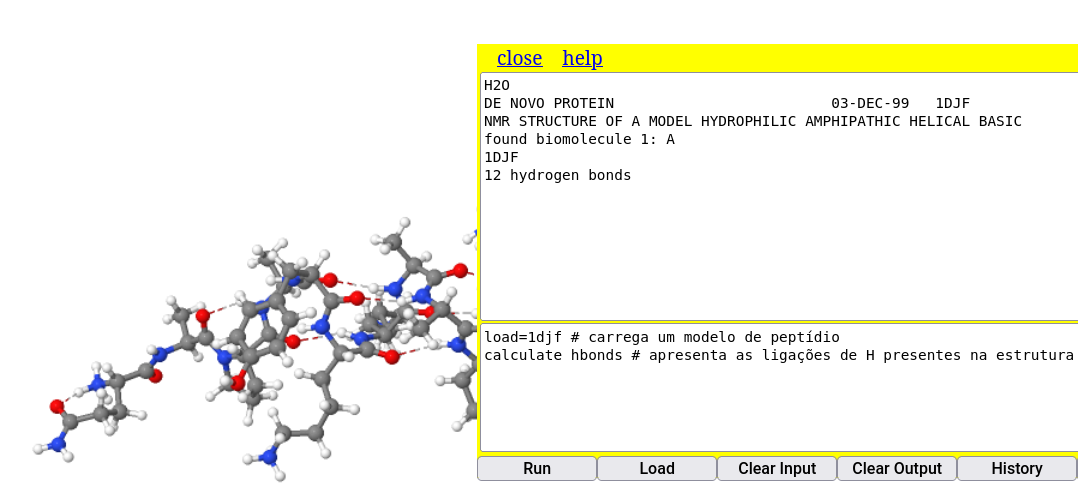
\includegraphics{ligacoesH.png}

}

\caption{Exemplificando ligações de hidrogênio num modelo de peptídio.}

\end{figure}%

\section{Superfícies}\label{superfuxedcies}

~~~~~~Além da superfície de van der Walls (\emph{dots on}) vista acima,
o \emph{Jmol} é capaz de representar algumas superfícies para modelos
moleculares. Quanto maior a molécula, maior o cálculo interno para gerar
a superfície, o que pode dificultar sua visualização. Assim, ilustrando
algumas superfícies para a molécula de água:

\begin{Shaded}
\begin{Highlighting}[]
\NormalTok{isosurface molecular }\CommentTok{\# superfície molecular que inclui o solvente}
\end{Highlighting}
\end{Shaded}

\begin{figure}[H]

{\centering 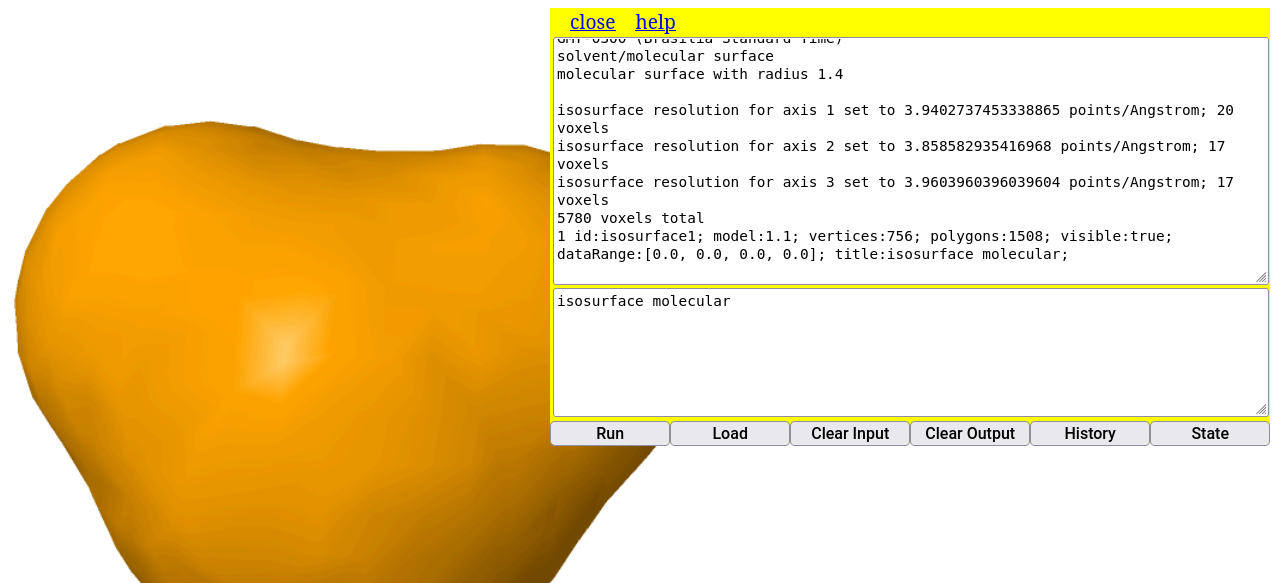
\includegraphics{isosurfMolec.png}

}

\caption{Superfície molecular para o modelo da água.}

\end{figure}%

\begin{Shaded}
\begin{Highlighting}[]
\NormalTok{isosurface mep }\CommentTok{\# superfície de potencial eletrostático molecular}
\end{Highlighting}
\end{Shaded}

\begin{figure}[H]

{\centering 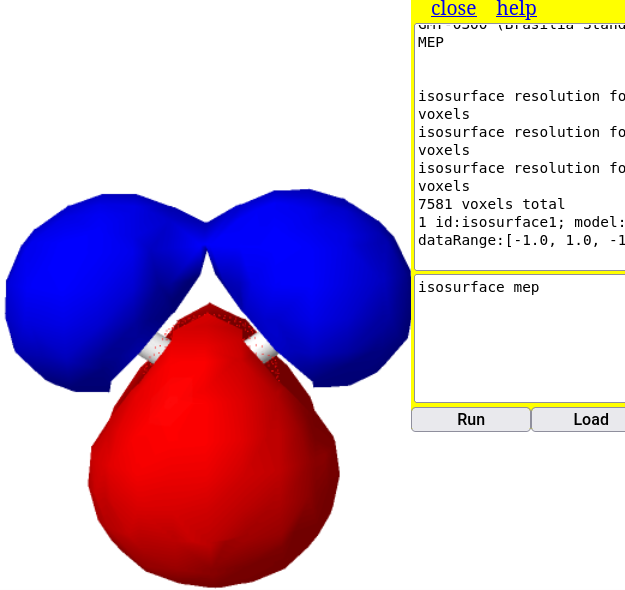
\includegraphics{isosurfMep.png}

}

\caption{Exemplo de superfície de potencial eletrostático para a água.}

\end{figure}%

\begin{Shaded}
\begin{Highlighting}[]
\NormalTok{isosurface resolution }\DecValTok{6}\NormalTok{ molecular map mep }\CommentTok{\# superfície de potencial eletrostático molecular com atributos}
\end{Highlighting}
\end{Shaded}

\begin{figure}[H]

{\centering 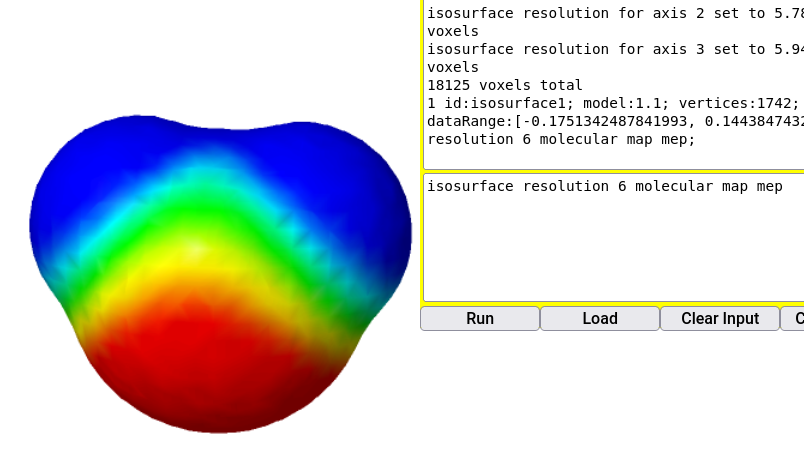
\includegraphics{isosurfFull.png}

}

\caption{Exemplo de superfície molecular da água que inclui seu
potencial eletrostático.}

\end{figure}%

~~~~~~Várias outras combinações de superfície podem ser obtidas no
{[}\emph{site} de referência do
\emph{Jmol}.(https://chemapps.stolaf.edu/jmol/docs/)

\bookmarksetup{startatroot}

\chapter{Seleção de partes da
molécula}\label{seleuxe7uxe3o-de-partes-da-moluxe9cula}

\section{Seleção de átomos e
visualização}\label{seleuxe7uxe3o-de-uxe1tomos-e-visualizauxe7uxe3o}

~~~~~~Por vezes faz-se interessante ou necessário chamar a atenção para
partes específicas de um modelo, como um átomo, grupo de átomos, uma
molécula pequena no interior de uma maior, entre outras situações. Nessa
seção serão vistos alguns comandos para isso.

~~~~~~O \emph{Jmol} foi concebido para estruturas mais complexas, como
proteínas e polímeros, razão pela qual a maior parte dos comandos de
seleção refiram-se a partes de proteínas e ácidos nucleicos.Contudo,
pode-se selecionar átomos ou grupo desses em moléculas pequenas, também.

\subsection{\texorpdfstring{Por
\emph{mouse}}{Por mouse}}\label{por-mouse}

~~~~~~Usando o \emph{mouse} pode-se selecionar um átomo por vez ou grupo
de átomos (esse no \emph{Jmol} do computador), como segue:

\begin{Shaded}
\begin{Highlighting}[]
\FloatTok{1.}\NormalTok{ Átomo }\SpecialCharTok{{-}}\NormalTok{ basta clicar em algum no ecrã (modelo);}
\FloatTok{2.}\NormalTok{ Grupo de átomos }\SpecialCharTok{{-}}\NormalTok{ Shift }\SpecialCharTok{+}\NormalTok{ clique botão esquerdo }\SpecialCharTok{+}\NormalTok{ arraste pra agrupar os átomos }\CommentTok{\# funciona no Jmol instalado no PC}
\end{Highlighting}
\end{Shaded}

\subsection{Por linha de comando}\label{por-linha-de-comando}

~~~~~~Por digitação do código consegue-se uma operação bem mais
abrangente que por clique de \emph{mouse}, incluindo o agrupamento de
átomos ou seleção daqueles com características comuns:

\begin{Shaded}
\begin{Highlighting}[]
\NormalTok{select }\StringTok{"propriedade do átomo"}
\end{Highlighting}
\end{Shaded}

~~~~~~Essas características são listadas abaixo:

\begin{Shaded}
\begin{Highlighting}[]
\NormalTok{todos os átomos}\SpecialCharTok{:}\NormalTok{ all }
\NormalTok{nenhum átomo}\SpecialCharTok{:}\NormalTok{ none}
\NormalTok{solvente}\SpecialCharTok{:}\NormalTok{ solvent}
\NormalTok{água}\SpecialCharTok{:}\NormalTok{ water ou hoh}
\NormalTok{íons}\SpecialCharTok{:}\NormalTok{ ions}
\NormalTok{átomo por símbolo atômico}\SpecialCharTok{:}\NormalTok{ \_N, \_C, \_Fe}
\NormalTok{átomo por número atômico}\SpecialCharTok{:}\NormalTok{ elemNo}\OtherTok{=}\DecValTok{7}
\NormalTok{átomo por identificação na sequência}\SpecialCharTok{:}\NormalTok{ atomNo}\SpecialCharTok{\textless{}}\DecValTok{50}

\CommentTok{\# Para biomoléculas:}
\NormalTok{proteína}\SpecialCharTok{:}\NormalTok{ protein}
\NormalTok{ácido nucleico}\SpecialCharTok{:}\NormalTok{ nucleic}
\NormalTok{DNA}\SpecialCharTok{:}\NormalTok{ dna}
\NormalTok{purina}\SpecialCharTok{:}\NormalTok{ purine}
\NormalTok{pirimidina}\SpecialCharTok{:}\NormalTok{ pyrimidine}
\NormalTok{carboidrato}\SpecialCharTok{:}\NormalTok{ carbohydrate}
\NormalTok{aminoácido}\SpecialCharTok{:}\NormalTok{ amino}


\CommentTok{\# Para aminoácidos numa proteína:}
\NormalTok{abreviação de }\DecValTok{3}\NormalTok{ letras}\SpecialCharTok{:}\NormalTok{ his, tyr, leu, etc}
\NormalTok{grandes}\SpecialCharTok{:}\NormalTok{ large}
\NormalTok{pequenos}\SpecialCharTok{:}\NormalTok{ small}
\NormalTok{ácidos}\SpecialCharTok{:}\NormalTok{ acidic}
\NormalTok{básicos}\SpecialCharTok{:}\NormalTok{ basic}
\NormalTok{polares}\SpecialCharTok{:}\NormalTok{ polar}
\NormalTok{apolares}\SpecialCharTok{:}\NormalTok{ hydrophobic}
\NormalTok{alifáticos}\SpecialCharTok{:}\NormalTok{ aliphatic}
\NormalTok{hidrofílicos}\SpecialCharTok{:}\NormalTok{ hydrophilic}
\NormalTok{aromáticos}\SpecialCharTok{:}\NormalTok{ aromatic}
\NormalTok{neutros}\SpecialCharTok{:}\NormalTok{ neutral}
\NormalTok{carregados}\SpecialCharTok{:}\NormalTok{ charged}
\NormalTok{na superfície}\SpecialCharTok{:}\NormalTok{ surface}
\NormalTok{no interior}\SpecialCharTok{:}\NormalTok{ buried}
\NormalTok{cistina}\SpecialCharTok{:}\NormalTok{ cystine}
\NormalTok{hem }\SpecialCharTok{{-}}\NormalTok{ grupo heme de ferroproteínas}

\CommentTok{\# Para proteínas}
\NormalTok{esqueleto carbônico de resíduos de aminoácidos}\SpecialCharTok{:}\NormalTok{ backbone ou spine}
\NormalTok{cadeia lateral de resíduos de aminoácidos}\SpecialCharTok{:}\NormalTok{ sidechain}
\NormalTok{átomos distintos dos presentes nos resíduos de aminoácidos}\SpecialCharTok{:}\NormalTok{ hetero}
\NormalTok{estruturas secundárias}\SpecialCharTok{:}\NormalTok{ helix, sheet, turn}
\end{Highlighting}
\end{Shaded}

\section{E depois de selecionar átomos, o que é que eu faço
?!}\label{sec-selecao}

~~~~~~Muuiiiitaaa coisa, também ! As instruções sequenciais abaixo
(\emph{scripts}) ilustram algumas possibilidades de se observar detalhes
de um modelo molecular com o \emph{Jmol}. Você pode copiar e colar no
\emph{Console} para observar os resultados.

\begin{Shaded}
\begin{Highlighting}[]
\CommentTok{\# Para colorir ligações as do metano}

\NormalTok{load }\SpecialCharTok{$}\NormalTok{methane }\CommentTok{\# carrega o modelo ...ou load $C}
\NormalTok{color bonds yellow }\CommentTok{\# coloração para as ligações}
\end{Highlighting}
\end{Shaded}

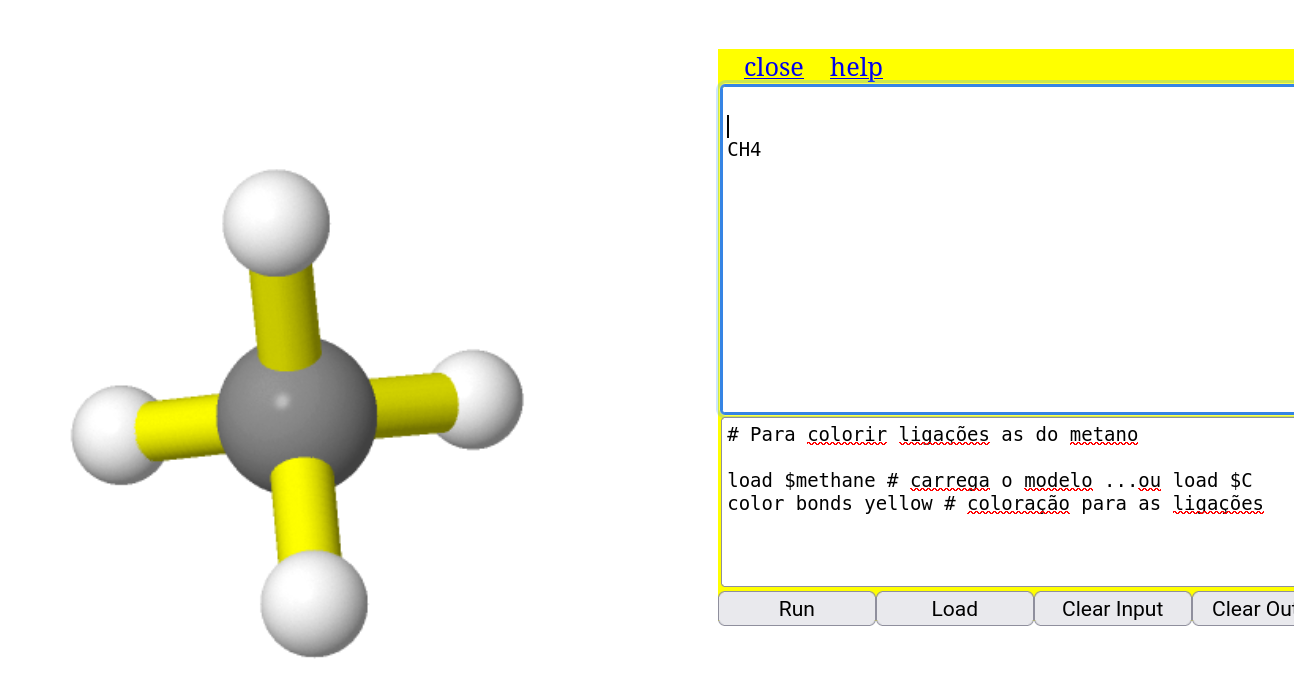
\includegraphics{metano.png}

\begin{Shaded}
\begin{Highlighting}[]
\CommentTok{\# Para nomear os átomos do tylenol e padronizar uma cor}

\NormalTok{load }\SpecialCharTok{$}\NormalTok{tylenol }\CommentTok{\# carrega o fármaco}
\NormalTok{label \%e }
\NormalTok{color shapely }\CommentTok{\# coloração única }
\end{Highlighting}
\end{Shaded}

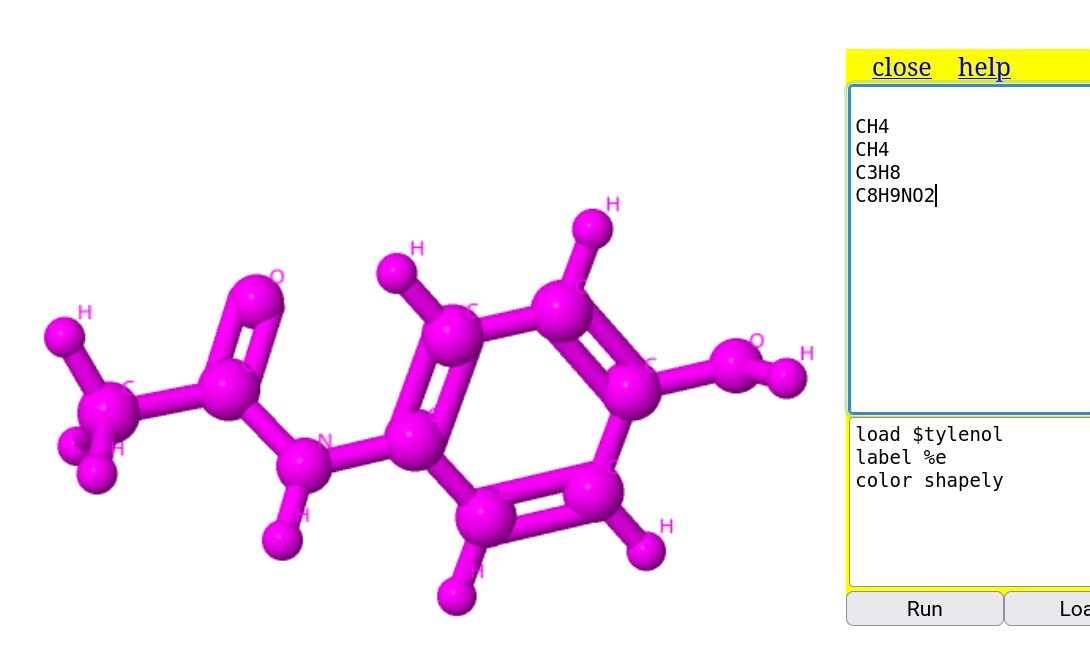
\includegraphics{tylenol.png} \textbar{} Aqui vale uma observação sobre
a etiquetagem dos átomos (nomes de cada no ecrã). Veja que não há
comentário seguindo a instrução. Isso é necessário para que o comentário
não seja a própria etiquetagem, e sim o símbolo do elemento.

\begin{Shaded}
\begin{Highlighting}[]
\CommentTok{\# Para selecionar e colorir os átomos de H}

\NormalTok{load }\SpecialCharTok{$}\NormalTok{cyclopropane }\CommentTok{\# carrega o modelo}
\NormalTok{select \_H }\CommentTok{\# seleciona os átomos de hidrogênio}
\NormalTok{label \%e}
\NormalTok{color AlcianBlue}
\end{Highlighting}
\end{Shaded}

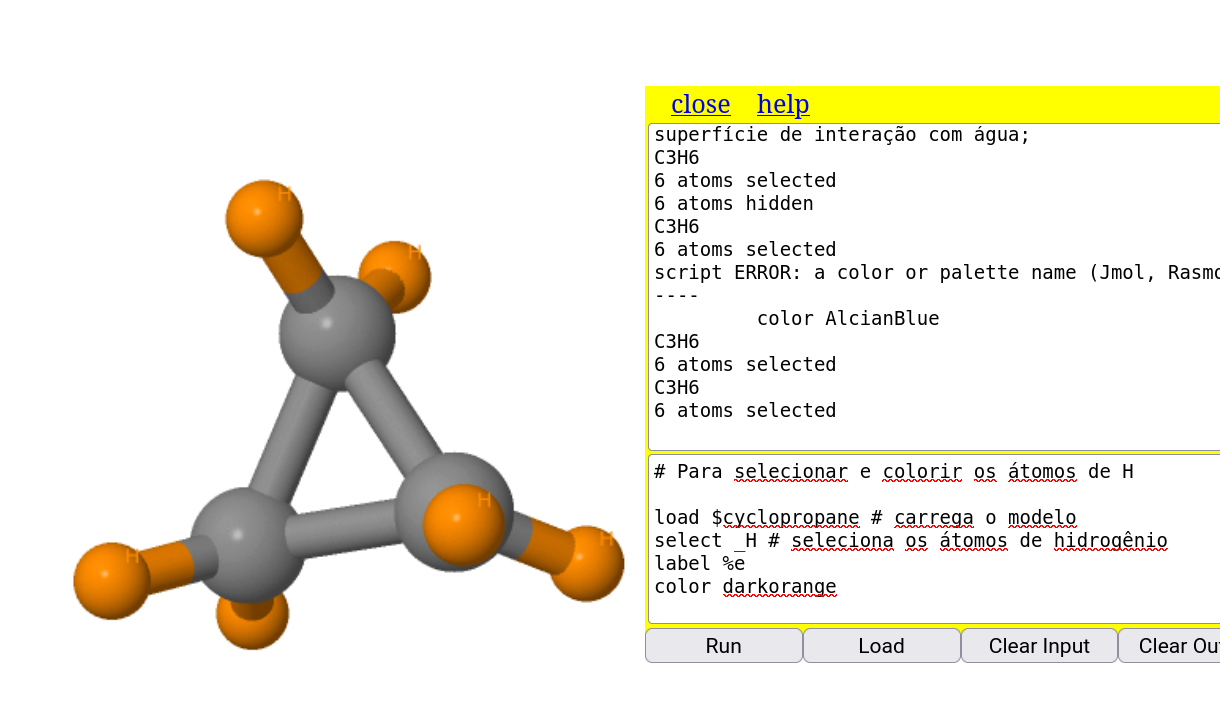
\includegraphics{ciclopropano.png}

\begin{Shaded}
\begin{Highlighting}[]
\CommentTok{\# Para selecionar e esconder os átomos de H de um propeno}

\NormalTok{load }\SpecialCharTok{$}\NormalTok{propene }\CommentTok{\# carrega o modelo}
\NormalTok{select \_H }\CommentTok{\# seleciona os átomos de H}
\NormalTok{hide selected }\CommentTok{\# esconde os átomos de H selecionados}
\end{Highlighting}
\end{Shaded}

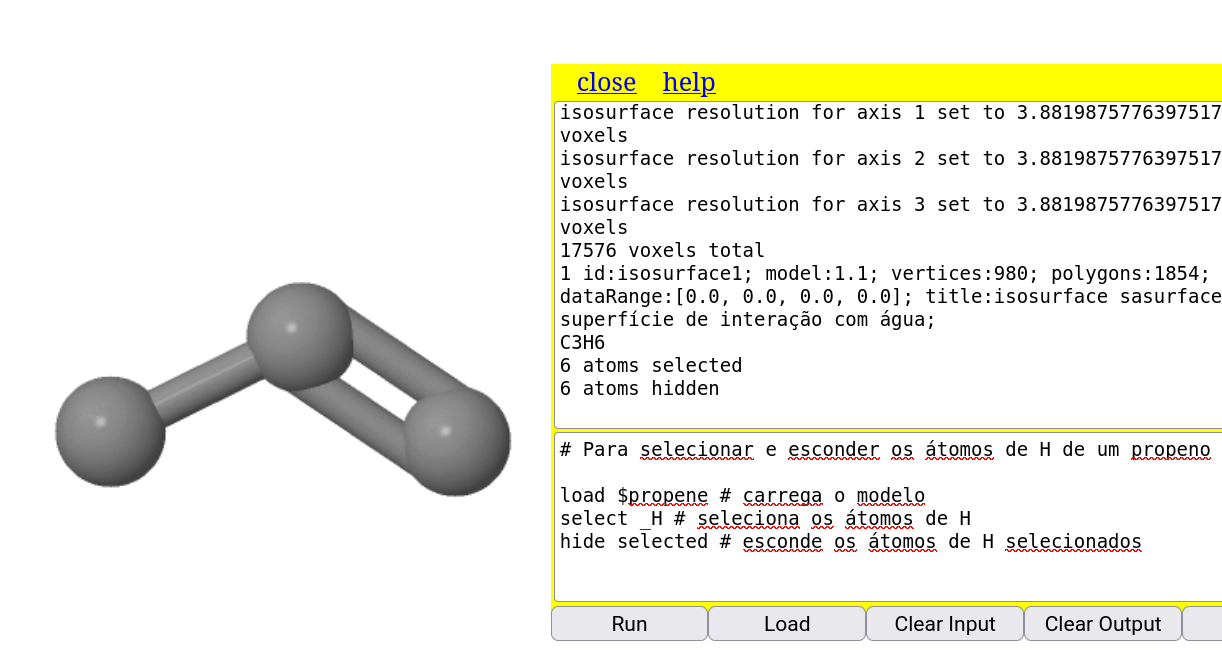
\includegraphics{propeno.png}

\begin{Shaded}
\begin{Highlighting}[]
\CommentTok{\# Para selecionar um átomo específico no modelo e apresentar sua área acessível ao solvente (SAS)}

\NormalTok{load }\SpecialCharTok{$}\NormalTok{urea}
\NormalTok{select atomno}\OtherTok{=}\DecValTok{2} \CommentTok{\# seleciona o carbono}
\NormalTok{label \%e }
\NormalTok{isosurface sasurface }\CommentTok{\# apresenta a superfície de interação com água}
\end{Highlighting}
\end{Shaded}

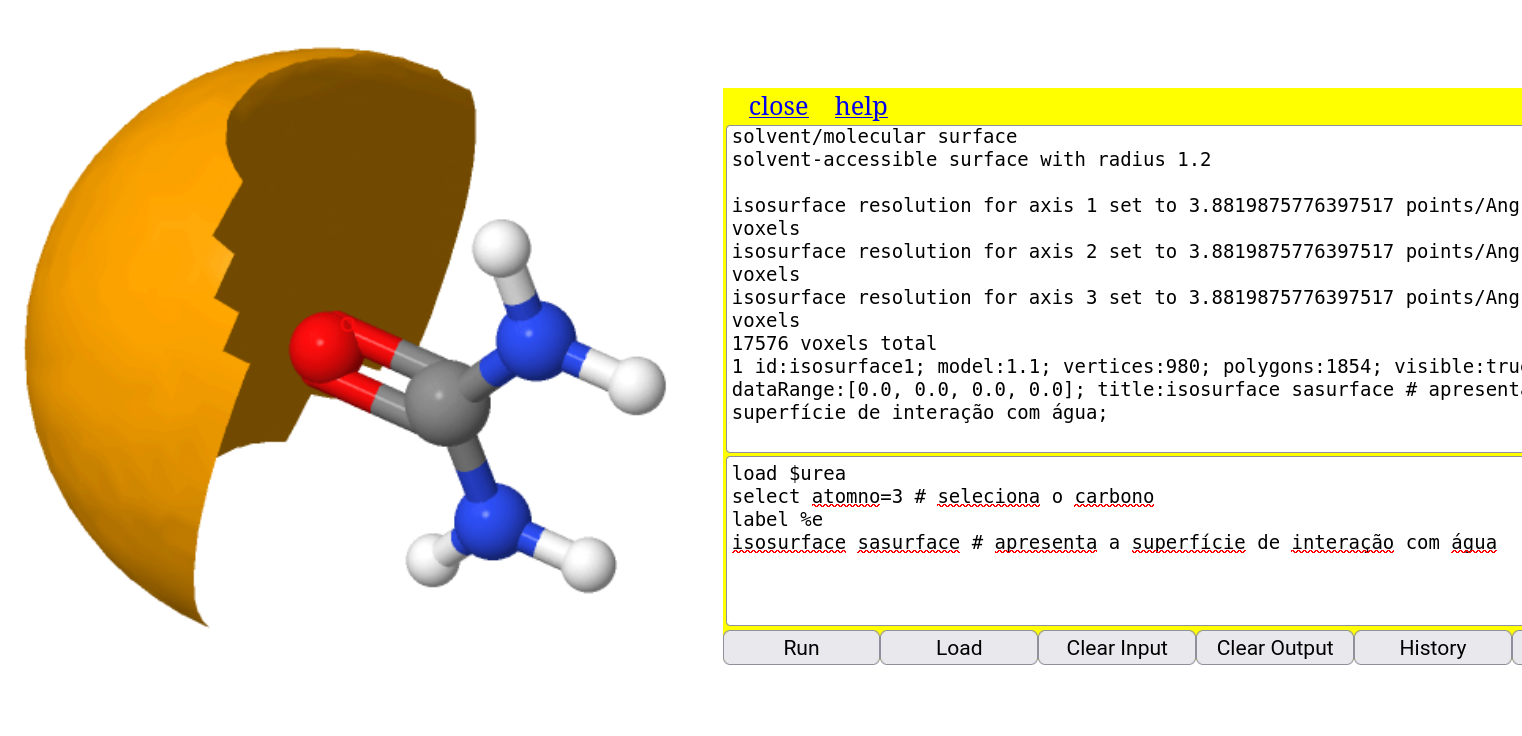
\includegraphics{urea.png}

\begin{Shaded}
\begin{Highlighting}[]
\CommentTok{\# Para ressaltar os carbonos de um hexadecano}

\NormalTok{load }\SpecialCharTok{$}\NormalTok{hexadecane }\CommentTok{\# carrega o modelo (ou...load $CCCCCC)}
\NormalTok{select carbon }\CommentTok{\# seleciona os C}
\NormalTok{color blue }\CommentTok{\# coloração azul}
\NormalTok{select hydrogen }\CommentTok{\# seleciona os H}
\NormalTok{color transparent }\CommentTok{\# reduz a visualização dos H}
\end{Highlighting}
\end{Shaded}

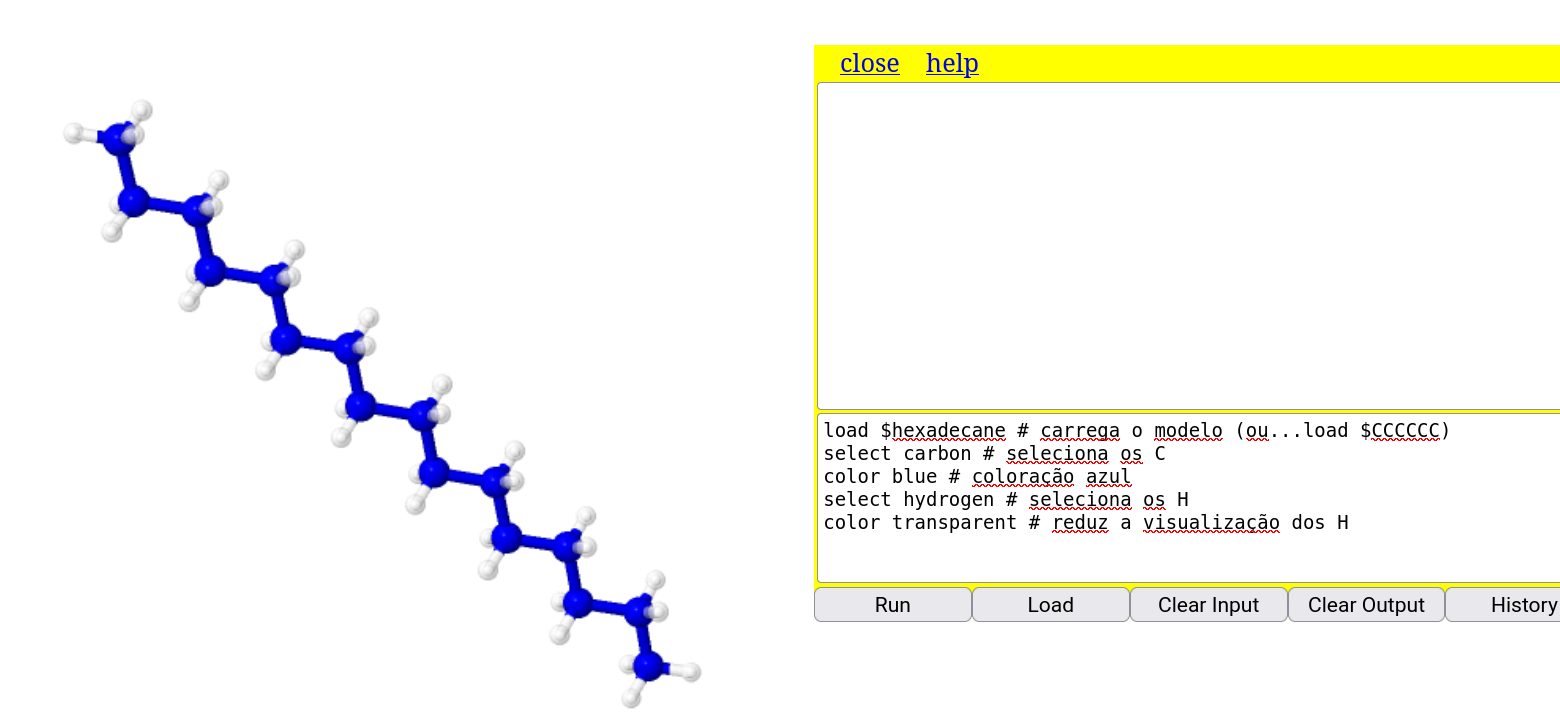
\includegraphics{hexadecano.png}

\begin{Shaded}
\begin{Highlighting}[]
\NormalTok{load}\OtherTok{=}\DecValTok{1}\NormalTok{crn }\CommentTok{\# carrega um modelo da proteína crambina}
\NormalTok{calculate hbonds }\CommentTok{\# apresenta as ligações de H presentes na estrutura}
\NormalTok{color hbonds Cyan }\CommentTok{\# coloração}
\NormalTok{hbonds }\FloatTok{0.5} \CommentTok{\# espessura da ligação de H}
\end{Highlighting}
\end{Shaded}

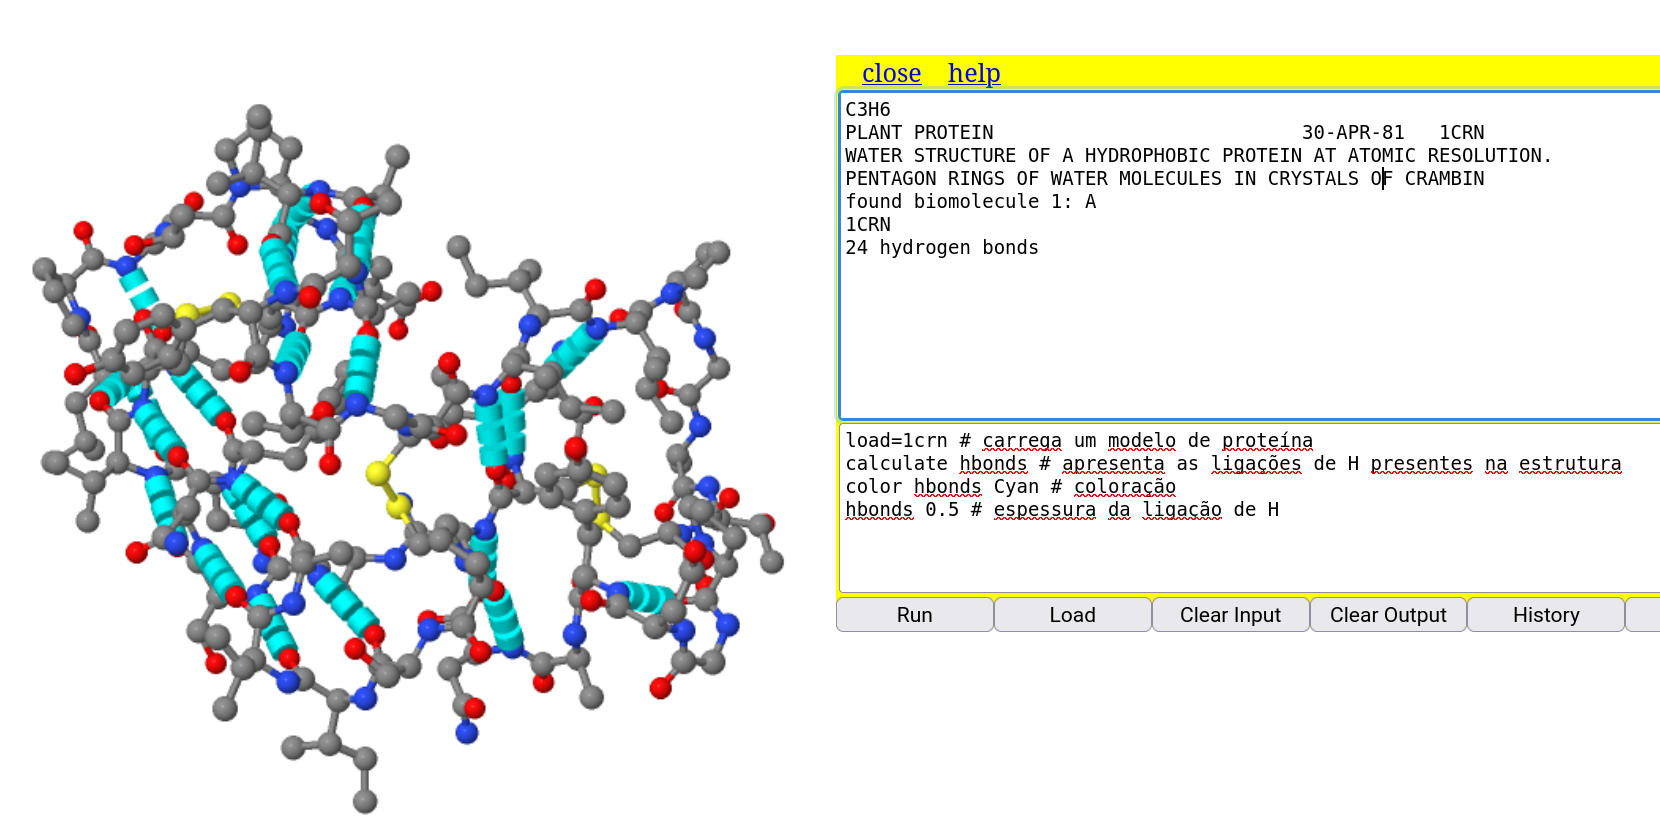
\includegraphics{hbondsCRN.png}

\begin{Shaded}
\begin{Highlighting}[]
\CommentTok{\# Superfíciel de potencial eletrostático para o fenol}

\NormalTok{load }\SpecialCharTok{$}\NormalTok{phenol }\CommentTok{\# carrega o modelo}
\NormalTok{isosurface solvent color range }\SpecialCharTok{{-}}\FloatTok{0.05} \FloatTok{0.05}\NormalTok{ map mep }\CommentTok{\# gera a superfície}
\NormalTok{color isosurface translucent }\FloatTok{0.5} \CommentTok{\# mantém a estrutura no interior}
\end{Highlighting}
\end{Shaded}

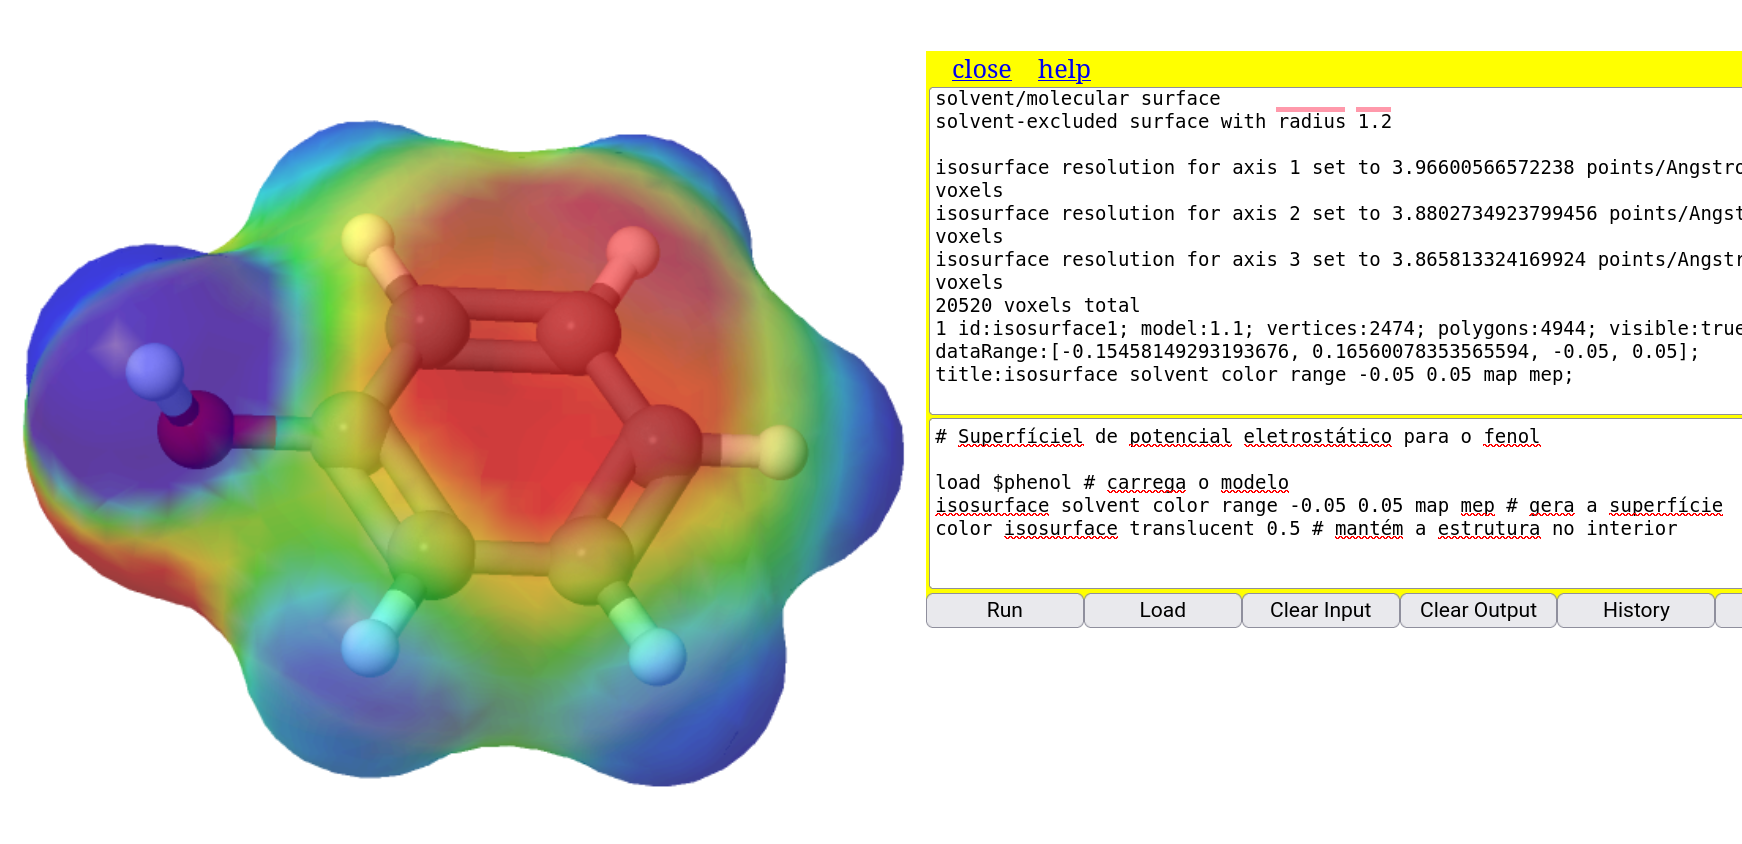
\includegraphics{fenol.png}

\bookmarksetup{startatroot}

\chapter{Animando a molécula}\label{animando-a-moluxe9cula}

\section{Alguns comandos de animação para os
modelos}\label{alguns-comandos-de-animauxe7uxe3o-para-os-modelos}

~~~~~~Animações permitem a representação de moléculas de modo mais
lúdico e representativo. Para agregar valor ainda maior à visualização
tridimensional de estruturas moleculares, o \emph{Jmol} conta com alguns
comandos para o posicionamento espacial do modelo, bem como para a
criação de animações, como:

\section{Rotacionar e transladar}\label{rotacionar-e-transladar}

~~~~~~Essas ações constituem uma forma simples de reposicionar o modelo
no espaço. Basta inserir o eixo e o ângulo em que se deseja o movimento
(\emph{x,y,z}). Ou apenas o ângulo, com o movimento padrão no eixo das
abscissas (\emph{X}). Seguem exemplos:

\begin{Shaded}
\begin{Highlighting}[]
\NormalTok{rotate }\DecValTok{20} \CommentTok{\# 20 graus}
\NormalTok{rotate x }\DecValTok{90} \CommentTok{\# eixo x}
\NormalTok{translate y }\DecValTok{50} \CommentTok{\# valor representa o percentual da janela (100 {-} fora; 0 {-} centro)}

\NormalTok{Obs}\SpecialCharTok{:}\NormalTok{ para retornar à posição original}\SpecialCharTok{:} \StringTok{\textasciigrave{}}\AttributeTok{reset}\StringTok{\textasciigrave{}}
\end{Highlighting}
\end{Shaded}

\section{Girar}\label{girar}

~~~~~~Essa ação, por sua vez, é mais ``impactante'', já que permite a
rotação do modelo a uma certa velocidade indefinidamente, até um comando
de parada. Como na anterior, pode-se digitar somente o comando para a
rotação padrão no eixo das abcissas, ou fornecer o eixo (\emph{x,y.z}):

\begin{Shaded}
\begin{Highlighting}[]
\NormalTok{spin }\DecValTok{10} \CommentTok{\# rotacional, com velocidade de 10 graus por quadro}
\NormalTok{spin z }\SpecialCharTok{{-}}\DecValTok{15} \CommentTok{\# (eixo z)}
\NormalTok{spin off }\CommentTok{\# interrompe a rotação}
\end{Highlighting}
\end{Shaded}

\section{\texorpdfstring{Ampliação dos modelos
(\emph{zoom})}{Ampliação dos modelos (zoom)}}\label{ampliauxe7uxe3o-dos-modelos-zoom}

~~~~~~É possível também ampliar ou reduzir o tamanho de uma molécula no
ecrã combinando-se o comando \texttt{zoom} à quantidades, tal como
segue:

\begin{Shaded}
\begin{Highlighting}[]
\NormalTok{Ampliação }\DecValTok{2}\NormalTok{x}\SpecialCharTok{:}\NormalTok{ zoom }\ControlFlowTok{in}
\NormalTok{Ampliação em }\DecValTok{3}\NormalTok{x}\SpecialCharTok{:}\NormalTok{ zoom }\SpecialCharTok{*}\DecValTok{3} 
\NormalTok{Redução em }\DecValTok{2}\NormalTok{x}\SpecialCharTok{:}\NormalTok{ zoom out }
\NormalTok{Redução em }\DecValTok{3}\NormalTok{x}\SpecialCharTok{:}\NormalTok{ zoom }\SpecialCharTok{/}\DecValTok{3} 
\NormalTok{Eliminar ampliação}\SpecialCharTok{:}\NormalTok{ zoom off }
\NormalTok{Restrição a um ligante e ampliação}\SpecialCharTok{:}\NormalTok{ restrict ligand; zoom }\DecValTok{0}

\NormalTok{Obs}\SpecialCharTok{:}\NormalTok{ para retornar ao tamanho original}\SpecialCharTok{:} \StringTok{\textasciigrave{}}\AttributeTok{zoom 0}\StringTok{\textasciigrave{}}
\end{Highlighting}
\end{Shaded}

~~~~~~Com ampliações, reduções, rotações, translações, é possível que
você queira retornar ao modelo na sua configuração de tamanho e
coordenadas originais. Para isto:

\begin{Shaded}
\begin{Highlighting}[]
\NormalTok{center; zoom }\DecValTok{0} \CommentTok{\# centraliza e redimensiona o modelo a seu tamanho original}
\end{Highlighting}
\end{Shaded}

\subsection{\texorpdfstring{Ampliação animada
(\emph{zoomTo})}{Ampliação animada (zoomTo)}}\label{ampliauxe7uxe3o-animada-zoomto}

~~~~~~Esse recurso é bem mais \emph{``chique''}, já que permite
visualizar de forma ampliada temporalmente algumas partes de interesse
do modelo. Isso é particularmente bacana com biomacromoléculas, como
para sítios de interação de ligantes ou grupos prostéticos, ou sítios de
reação em catálise enzimática. Mas também impacta a visualização de
pequenas moléculas, posto que os modelos crescem ou reduzem de forma
animada no ecrã; pode-se também focar num átomo específico para chamar a
atenção na molécula. A sintaxe da expressão é:

\begin{Shaded}
\begin{Highlighting}[]
\NormalTok{zoomto tempo tamanho }\CommentTok{\#...ou, se quiser um grupo de átomos em especial (ligante, por ex)...}
\NormalTok{zoomto }\FunctionTok{tempo}\NormalTok{ (expressão do átomo}\SpecialCharTok{/}\NormalTok{grupo) tamanho}
\end{Highlighting}
\end{Shaded}

~~~~~~Experimente carregar moléculas pequenas e proteínas, ilustrando o
comando \texttt{zoomTo} como segue:

\begin{Shaded}
\begin{Highlighting}[]
\NormalTok{Aumentar em }\DecValTok{3}\NormalTok{x, meio segundo por vez}\SpecialCharTok{:}\NormalTok{ zoomto }\FloatTok{0.5} \SpecialCharTok{*}\DecValTok{3} 
\NormalTok{Aumentar em }\DecValTok{4}\NormalTok{x, meio segundo por vez}\SpecialCharTok{:}\NormalTok{ zoomto }\FloatTok{0.5} \DecValTok{400} 
\NormalTok{Focar num ligante com ampliação de }\DecValTok{2}\NormalTok{x}\SpecialCharTok{:}\NormalTok{ zoomto }\DecValTok{2}\NormalTok{(ligand) }\DecValTok{0}
\NormalTok{Focar num ligante com ampliação de }\DecValTok{4}\NormalTok{x, a meio segundo por vez}\SpecialCharTok{:}\NormalTok{ zoomto }\FloatTok{0.5}\NormalTok{(ligand)}\SpecialCharTok{*} \DecValTok{4}
\end{Highlighting}
\end{Shaded}

\section{Pausa}\label{pausa}

~~~~~~Um comando muito interessante para o \emph{Jmol}, bem como para
outras linguagens de programação, é \texttt{delay}. Essa ação permite
que o \emph{script} interrompa uma ação por algum tempo, medido em
segundos, e limitado ao mínimo de um segundo. Experimente:

\begin{Shaded}
\begin{Highlighting}[]
\NormalTok{load }\SpecialCharTok{$}\NormalTok{ribose }\CommentTok{\# carrega uma ribose}
\NormalTok{spin }\DecValTok{50} \CommentTok{\# rotaciona no eixo X}
\NormalTok{delay }\DecValTok{5} \CommentTok{\# aguarda 5s}
\NormalTok{spin off }\CommentTok{\# interrompe a rotação}
\NormalTok{wireframe only }\CommentTok{\# represeta em arame, somente}
\NormalTok{wireframe }\DecValTok{130} \CommentTok{\# espesssura do arame}
\NormalTok{color translucent }\CommentTok{\# cor translúcida}
\end{Highlighting}
\end{Shaded}

\section{Laço}\label{lauxe7o}

~~~~~~O \emph{Jmol} possui alguns comandos normalmente utilizados em
linguagens de programação, embora não seja esse o escopo do presente
trabalho. Se quiser \emph{``ir fundo''}, consulte o
\href{https://chemapps.stolaf.edu/jmol/docs/}{manual de referência de
comandos do \emph{Jmol}} para os comandos de programação: \emph{if,
ifelse, for, while, step, break, wait, pause, case, continue, quit,
loop}.

~~~~~~Mas entre esses comandos variados, o de \emph{laço iterativo}
(\texttt{loop}) pode ser de valia ao ensino, por exemplo, para quando se
desejar chamar à atenção para uma ligação, um átomo ou grupo de átomos.
Exemplificando:

\begin{Shaded}
\begin{Highlighting}[]
\NormalTok{load }\SpecialCharTok{$}\NormalTok{acetate }\CommentTok{\# carrega um modelo de acetato}
\NormalTok{color bonds red }\CommentTok{\# coloração vermelha às ligações}
\NormalTok{delay }\DecValTok{1} \CommentTok{\# aguarda 1 segundo}
\NormalTok{color bonds green }\CommentTok{\# troca a coloração para verde}
\NormalTok{loop }\DecValTok{1} \CommentTok{\# realiza o laço (efeito "piscante")}
\end{Highlighting}
\end{Shaded}

~~~~~~Para deixar o laço, ou seja, interromper a sequência em
\emph{loop}, digita-se \emph{\texttt{quit}}.

\section{Combinando rotações, translações, e ampliações no
tempo}\label{combinando-rotauxe7uxf5es-translauxe7uxf5es-e-ampliauxe7uxf5es-no-tempo}

~~~~~~O \emph{Jmol} oferece dois comandos básicos para isso:
\texttt{move} e \texttt{moveTo}. A diferença é que \texttt{move}
reorienta o modelo em relação à sua posição atual (\emph{movimento
relativo}), e \texttt{moveTo} o faz em relação à posição original do
modelo (\emph{movimento absoluto}).

~~~~~~Na prática, contudo, o comando \texttt{move} é mais simples de
executar, dependendo somente de parâmetros de rotação e translação, ao
passo que \texttt{moveTo} é bem mais complexo. Esse depende de
parâmetros de orientação manualmente obtidos pelo \emph{Jmol}.

\subsection{Move}\label{move}

~~~~~~Para o comando \texttt{move} bastam os parâmetros que se deseja
modificar (\emph{nove} no total). Dependendo do que se deseja não há
necessidade de usar todos os parâmetros, e que são fornecidos abaixo:

\begin{Shaded}
\begin{Highlighting}[]
\NormalTok{move rotX rotY rotZ zoom dx dy dz slab time}

\NormalTok{Onde}\SpecialCharTok{:}
\NormalTok{  rotX, Y ou Z }\OtherTok{=}\NormalTok{ rotação no eixo X, Y, ou Z}
\NormalTok{  zoom }\OtherTok{=}\NormalTok{ ampliação ou redução}
\NormalTok{  dX, Y ou Z }\OtherTok{=}\NormalTok{ translação no eixo X, Y ou Z}
\NormalTok{  slab }\OtherTok{=}\NormalTok{ plano de fatiamento da molécula}
\NormalTok{  time }\OtherTok{=}\NormalTok{ tempo total envolvido no movimento}
\end{Highlighting}
\end{Shaded}

~~~~~~Seguem alguns exemplos:

\begin{Shaded}
\begin{Highlighting}[]
\NormalTok{move }\DecValTok{90} \DecValTok{180} \DecValTok{0} \DecValTok{0} \DecValTok{0} \DecValTok{0} \DecValTok{0} \DecValTok{0} \DecValTok{21} \CommentTok{\# rotaciona o modelo por 45 graus em torno do eixo X e por 180 graus no eixo Y, e empregando um movimento gradual de 2 segundos}
\NormalTok{move }\DecValTok{0} \DecValTok{0} \DecValTok{0} \DecValTok{0} \DecValTok{0} \DecValTok{35} \DecValTok{0} \DecValTok{0} \FloatTok{0.5} \CommentTok{\# reduz o modelo em 35\% de seu tamanho, e com movimento gradual de 0,5 segundos}
\NormalTok{move }\DecValTok{45} \DecValTok{0} \DecValTok{90} \DecValTok{150} \DecValTok{0} \DecValTok{30} \DecValTok{0} \DecValTok{0} \DecValTok{5} \CommentTok{\# rotaciona 45 graus no eixo X e 90 graus no eixo Z, ampliando o modelo em 150\% e transladando{-}o por 30\%, tudo ao longo de 5 segundos.}
\end{Highlighting}
\end{Shaded}

\subsection{MoveTo}\label{moveto}

~~~~~~Resulta em orientação \emph{absoluta} do modelo, não dependendo de
suas coordenadas anteriores. Sua inserção não é simples, pois depende
dos dados da orientação do modelo quando carregado pela 1a. vez, e que
pode ser obtida por:

\begin{Shaded}
\begin{Highlighting}[]
\NormalTok{show orientation}
\end{Highlighting}
\end{Shaded}

~~~~~~Um exemplo de resultado pelo comando é:

\begin{Shaded}
\begin{Highlighting}[]
\NormalTok{moveto }\SpecialCharTok{/}\ErrorTok{*}\NormalTok{ time, axisAngle }\SpecialCharTok{*}\ErrorTok{/} \FloatTok{1.0}\NormalTok{ \{ }\DecValTok{616} \SpecialCharTok{{-}}\DecValTok{708} \SpecialCharTok{{-}}\DecValTok{346} \FloatTok{47.68}\NormalTok{\} }\SpecialCharTok{/}\ErrorTok{*}\NormalTok{ zoom, translation }\SpecialCharTok{*}\ErrorTok{/}  \FloatTok{400.0} \FloatTok{0.0} \FloatTok{0.0}  \SpecialCharTok{/}\ErrorTok{*}\NormalTok{ center, rotationRadius }\SpecialCharTok{*}\ErrorTok{/}\NormalTok{ \{}\FloatTok{15.174467} \FloatTok{28.719118} \FloatTok{4.726837}\NormalTok{\} }\FloatTok{35.148052} \SpecialCharTok{/}\ErrorTok{*}\NormalTok{ navigation center, translation, depth }\SpecialCharTok{*}\ErrorTok{/}\NormalTok{ \{}\DecValTok{0} \DecValTok{0} \DecValTok{0}\NormalTok{\} }\DecValTok{0} \DecValTok{0} \DecValTok{0} \SpecialCharTok{/}\ErrorTok{*}\NormalTok{ cameraDepth, cameraX, cameraY }\SpecialCharTok{*}\ErrorTok{/}  \FloatTok{3.0} \FloatTok{0.0} \FloatTok{0.0}\NormalTok{;}
\CommentTok{\#OR}
\CommentTok{\#Follows Z{-}Y{-}Z convention for Euler angles}
\NormalTok{reset;center \{}\FloatTok{15.174467} \FloatTok{28.719118} \FloatTok{4.726837}\NormalTok{\}; rotate z }\FloatTok{130.27}\NormalTok{; rotate y }\FloatTok{44.57}\NormalTok{; rotate z }\SpecialCharTok{{-}}\FloatTok{147.67}\NormalTok{; zoom }\FloatTok{400.0}\NormalTok{;}
\end{Highlighting}
\end{Shaded}

~~~~~~Perceba que há dois conjuntos de comandos um pelo \emph{moveTo} e
outro por \emph{reset, center, rotate e translate}. Para obter o modelo
nas coordenadas originais, basta copiar um ou outro conjunto de dados.

~~~~~~Usando-se o 1o. conjunto (\emph{moveTo}), copia-se a linha e
altera-se o tempo de animação, no caso o valor 1.0 em ``axisAngle */
1.0''.

\section{Comparando dois modelos no
ecrã}\label{comparando-dois-modelos-no-ecruxe3}

~~~~~~Compara 2 modelos e reorienta as coordenadas do segundo para
justapor-se ao primeiro, por um algoritmo de correlação.

\begin{Shaded}
\begin{Highlighting}[]
\NormalTok{load files }\StringTok{"$tyrosine"} \StringTok{"$epinephrine"}\NormalTok{;}
\NormalTok{frame }\SpecialCharTok{*}\NormalTok{;}
\NormalTok{compare \{}\FloatTok{2.1}\NormalTok{\} \{}\FloatTok{1.1}\NormalTok{\} rotate translate }\FloatTok{5.0} 
\end{Highlighting}
\end{Shaded}

\section{Navigate}\label{navigate}

~~~~~~O comando permite explorar o modelo simulando um passeio
panorâmico ao interior da estrutura. Os parâmetros envolvem o tempo de
percuro (ou 2s quando omitido). Exemplificando:

\begin{Shaded}
\begin{Highlighting}[]
\NormalTok{navigate depth }\DecValTok{50} \CommentTok{\# imersão no modelo em 2s}
\NormalTok{navigate }\DecValTok{3}\NormalTok{ rotate y }\DecValTok{20} \CommentTok{\# rotaciona 20o no eixo y}
\NormalTok{navigate }\DecValTok{4}\NormalTok{ trace }\CommentTok{\# passeia pelo modelo em 4s}
\NormalTok{navigate }\DecValTok{3}\NormalTok{ translate \{}\DecValTok{30} \DecValTok{50} \DecValTok{70}\NormalTok{\} modelo translada levemente por }\DecValTok{3}\NormalTok{s}
\NormalTok{navigate }\DecValTok{5}\NormalTok{ center \{}\DecValTok{10} \DecValTok{20} \DecValTok{30}\NormalTok{\} }\CommentTok{\# sonda ao lado do modelo, e nas coordenadas x, y, z}
\NormalTok{navigate }\DecValTok{2}\NormalTok{ depth }\DecValTok{30} \SpecialCharTok{/} \DecValTok{5}\NormalTok{ rotate }\DecValTok{180} \SpecialCharTok{/}\NormalTok{ depth }\DecValTok{20} \SpecialCharTok{/}\NormalTok{ translate X }\DecValTok{10}
\end{Highlighting}
\end{Shaded}

\section{\texorpdfstring{Exemplos de animações para moléculas no
\emph{Jmol}}{Exemplos de animações para moléculas no Jmol}}\label{exemplos-de-animauxe7uxf5es-para-moluxe9culas-no-jmol}

\part{PARTE 2 - R \& RStudio}


\includegraphics[width=2\textwidth,height=\textheight]{RPart.png}

\bookmarksetup{startatroot}

\chapter{Como usar o R \& Rstudio - instalação e
nuvem}\label{como-usar-o-r-rstudio---instalauxe7uxe3o-e-nuvem}

~~~~~~Existem dois ambientes alternativos para se utilizar o \emph{R}
(programa) e o \emph{Rstudio} (interface do usário): instalando no
computador, ou pelas nuvens. Há poucas diferenças entre ambas as
maneiras de se trabalhar com os programas, mas a fundamental é que a
\emph{instalação} pode ser utilizada \emph{offline}, sem necessidade de
internet, enquanto que pelas nuvens, bom, já sabe.

\section{Instalando o R e RStudio no
computador}\label{instalando-o-r-e-rstudio-no-computador}

~~~~~~Você precisa seguir uns poucos passos para instalar o \emph{R \&
RStudio} no computador. Na prática, baixa-se ambos os programas e os
instala como se faria com qualquer outro programa, tanto faz se para
\emph{Windows}, \emph{Linux}, ou \emph{Mac}. Seguem os passos:

\begin{enumerate}
\def\labelenumi{\arabic{enumi}.}
\item
  Acesse o site do
  \href{https://posit.co/download/rstudio-desktop/}{Rstudio} e faça o
  \emph{download} do programa \texttt{R}.
  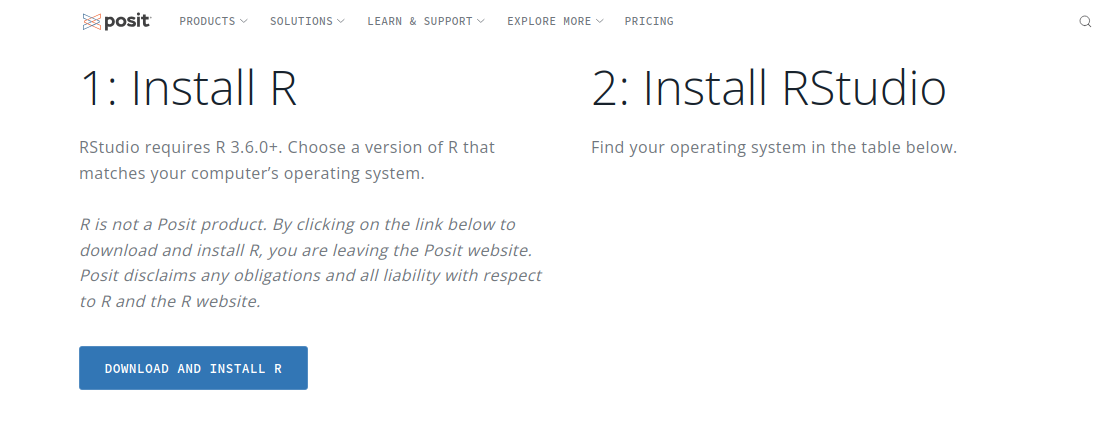
\includegraphics{rstudioSite.png}
\item
  Instale o programa com as opções padrão.
\item
  No mesmo site do
  ´\href{https://posit.co/download/rstudio-desktop/}{RStudio} procure um
  pouco mais abaixo pelo instalador mais apropriado a seu sistema
  operacional.
\end{enumerate}

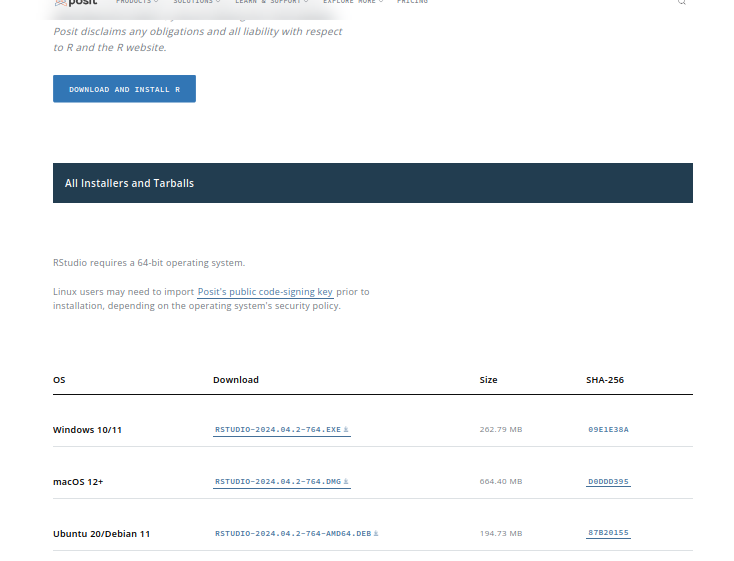
\includegraphics{rstudioInstala.png}

\begin{enumerate}
\def\labelenumi{\arabic{enumi}.}
\setcounter{enumi}{2}
\item
  Baixe o arquivo e instale-o como qualquer outro programa.
\item
  Abra o programa \emph{RStudio}, e cuja interface será parecida com a
  que segue.
\end{enumerate}

\begin{figure}

\centering{

\captionsetup{labelsep=none}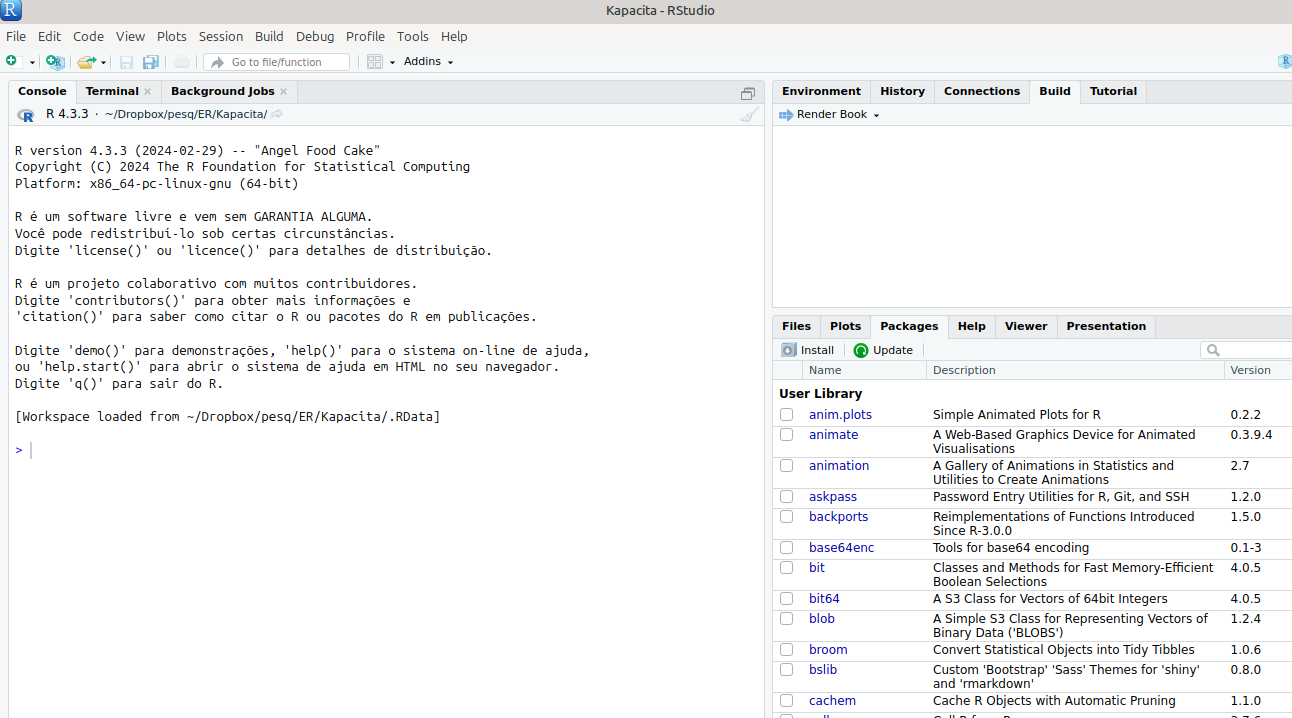
\includegraphics{rstudioJanela.png}

}

\caption{\label{fig-rstudioJanela}}

\end{figure}%

\section{\texorpdfstring{Acessando o \texttt{R\ \&\ Rstudio} pelas
nuvens}{Acessando o R \& Rstudio pelas nuvens}}\label{acessando-o-r-rstudio-pelas-nuvens}

~~~~~~Essa é uma opção simples e que não requer qualquer instalação. A
interface acessada é praticamente igual à da instalação em computador.
Entre algumas vantagens destaca-se a velocidade normalmente superior pra
rodar e instalar pacotes, posto que o servidor para esses já está no
provedor em nuvem. Mas por ser acesso \emph{online}, requer uma
inscrição inicial, com \emph{login e senha}. Seguem os passos:

\begin{enumerate}
\def\labelenumi{\arabic{enumi}.}
\tightlist
\item
  Acesse o site do
  \href{https://login.posit.cloud/login?redirect=\%2Foauth\%2Fauthorize\%3Fredirect_uri\%3Dhttps\%253A\%252F\%252Fposit.cloud\%252Flogin\%26client_id\%3Dposit-cloud\%26response_type\%3Dcode\%26show_auth\%3D0}{RStudio
  Cloud}.
\end{enumerate}

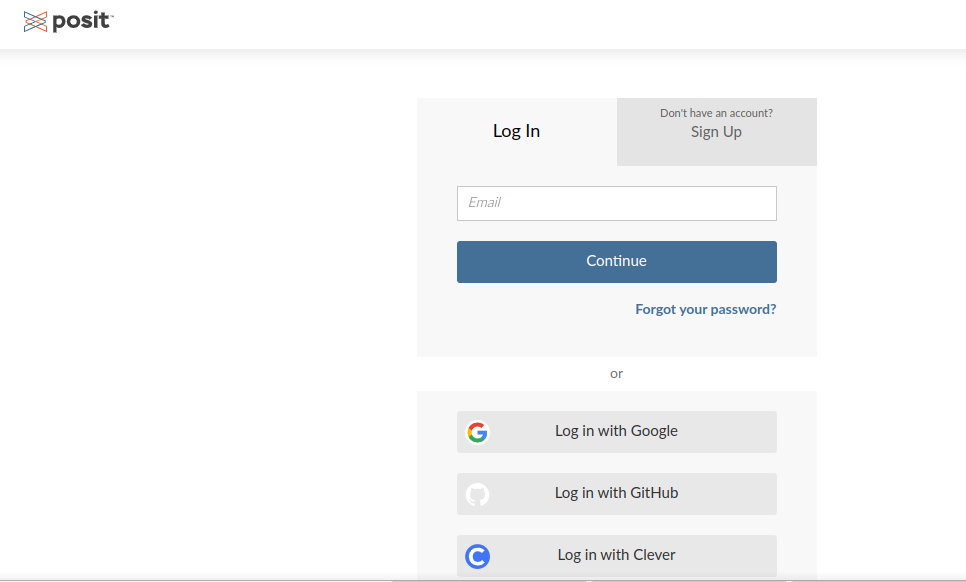
\includegraphics{rstudioNuvem.png}

\begin{enumerate}
\def\labelenumi{\arabic{enumi}.}
\setcounter{enumi}{1}
\item
  Realize a inscrição (\emph{sign up}) ou acesse pelo \emph{Google}
  (mais simples).
\item
  A janela deverá parecer-se com a que segue, embora sem os projetos
  listados.
\end{enumerate}

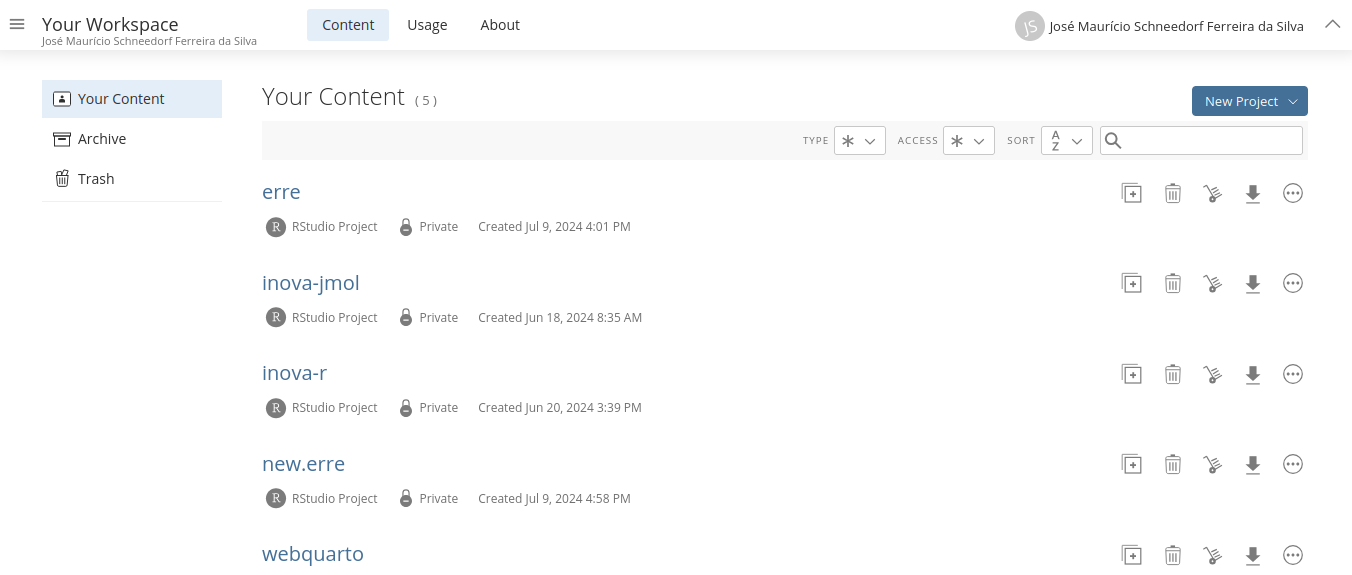
\includegraphics{rstudioCloudMain.pdf}

\begin{enumerate}
\def\labelenumi{\arabic{enumi}.}
\setcounter{enumi}{3}
\tightlist
\item
  Agora a parte interessante. Clique em \emph{New Project} e selecione
  \emph{New Rstudio Project}.
\end{enumerate}

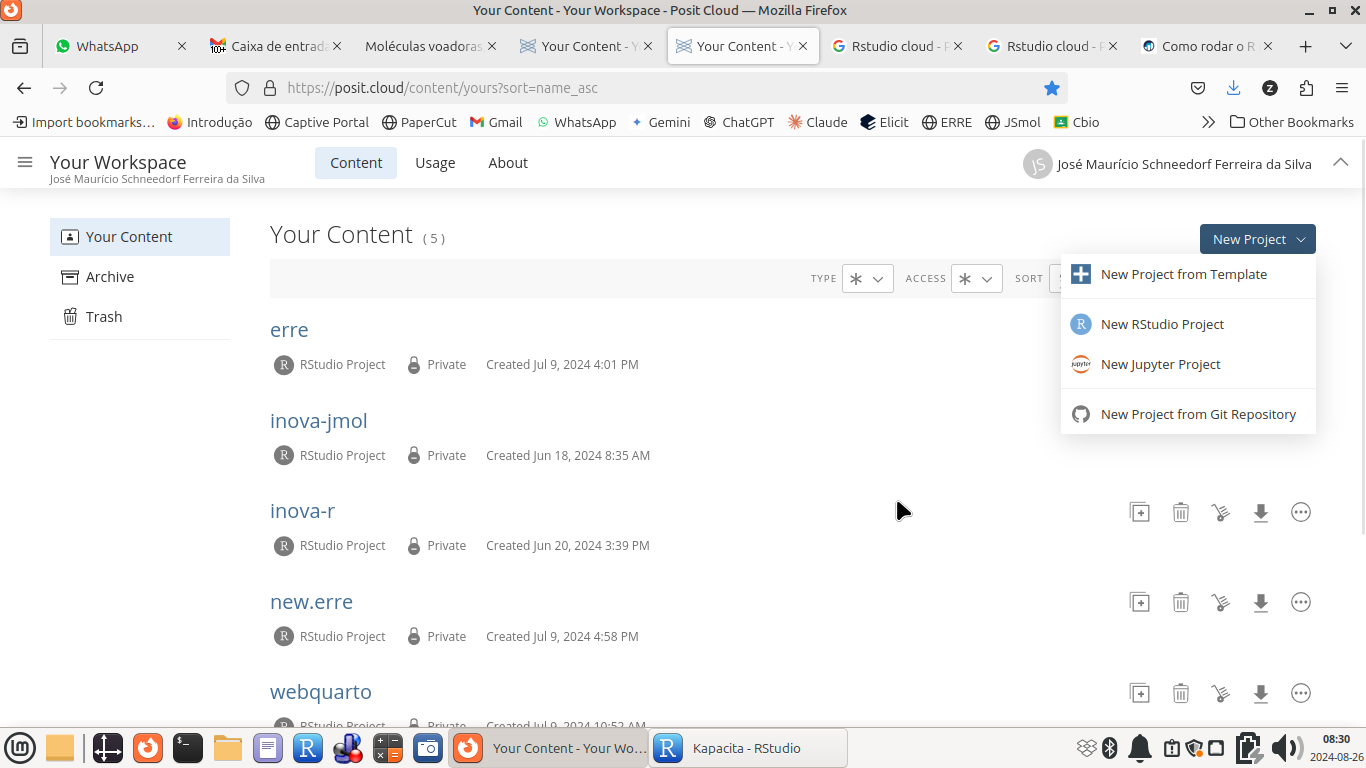
\includegraphics{rstudioCloudNewProj.png}

\begin{enumerate}
\def\labelenumi{\arabic{enumi}.}
\setcounter{enumi}{4}
\tightlist
\item
  A imagem final será bem parecida com a apresentada pela versão
  instalada, como visto na Figura~\ref{fig-rstudioJanela}, veja:
\end{enumerate}

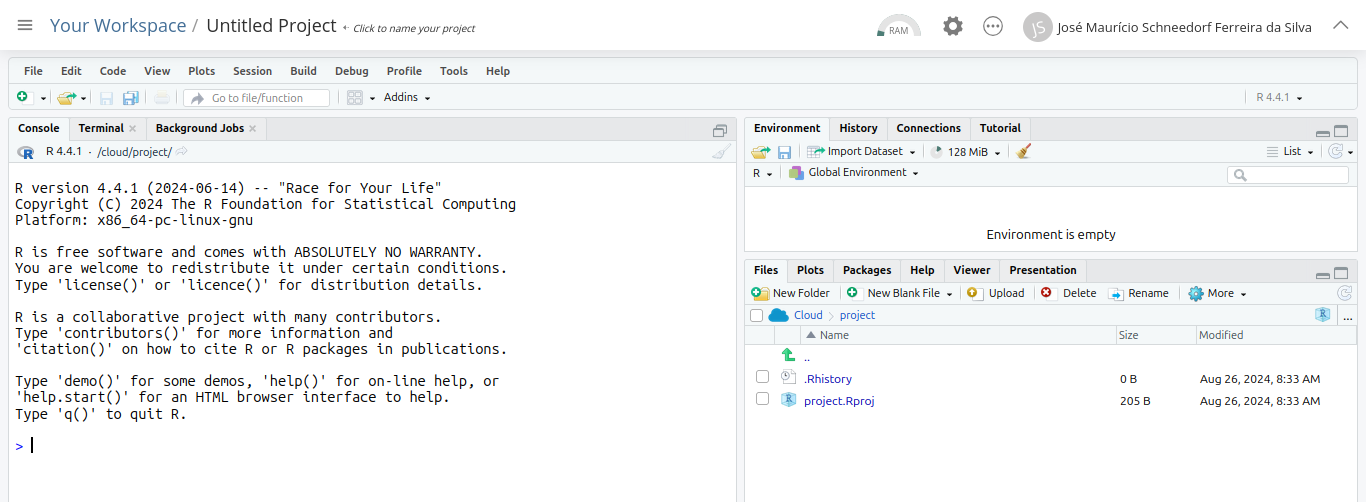
\includegraphics{rstudioCloudFinal.png} \textbar{} Pronto ! Você pode
utilizar uma ou outra forma para acessar as atividades e objetos
didáticos propostos neste material. A seguir serão fornecidas algumas
ações e comandos rápidos para se trabalhar com a interface do
\texttt{Rstudio} e com o \texttt{R}. Mas apenas para que se consiga
criar, executar, e modificar alguns \emph{scripts} criados para
animações, simulações, interatividade, e geovisualização. Mão na massa,
agora !

~~~~~~Por uma questão de simplicidade para o uso da versão em servidor,
sem necessidade de instalação dos programas, bem como por maior
velocidade de execução de \emph{scripts} e instalação de pacotes,
optamos neste trabalho por exemplificar os \emph{objetos didáticos} em
nuvem, ou seja, por uso do \href{https://posit.cloud/}{RStudio Cloud}.

\bookmarksetup{startatroot}

\chapter{Comandos básicos \& Scripts no
R}\label{comandos-buxe1sicos-scripts-no-r}

~~~~~~O \texttt{R} é um programa que opera por linha de comando. Isso é
um pouco chato, como já visto, porque qualquer erro na digitação de um
comando resulta na interrupção do código. Mas, por outro lado, e também
como já visto, \emph{linhas de comando encadeadas e comentadas permitem
a reprodução e modificação de trechos de códigos convergentes a um
produto} qualquer, no caso, objetos didáticos ao ensino médio.

~~~~~~Diferente do \emph{Jmol}, contudo, não é possível mesclar fonte
maiúsculas ou minúsculas, bem como singular ou plural. Para que o código
funcione, é necessário sua correta digitação. Mas \emph{pode-se
tranquilamente aumentar ou reduzir o espaço entre comandos}, o que não
faz diferença pro compilador do \texttt{R}.

~~~~~~Algumas operações são realizadas alternativamente por
\emph{mouse}, \emph{linha de comando}, ou ambos, dependendo da ação. A
seguir serão apresentadas algumas funcionalidades básicas para a
reprodução de códigos para objetos didáticos, sem descrições detalhadas
da operação própria do \emph{R \& RSTudio}, para simplificar e tornar
mais objetivo este trabalho. Se você desejar saber mais a respeito de
ambos os programas, versão instalada ou em nuvem, sugerimos os inúmeros
sites e tutoriais disponíveis na internet, bem como centenas de livros
já escritos no assunto, e cursos \emph{on-line} em várias plataformas de
ensino.

\hfill\break

\section{\texorpdfstring{Uma visão da interface
\emph{RStudio}}{Uma visão da interface RStudio}}\label{uma-visuxe3o-da-interface-rstudio}

\hfill\break
\textbar{} O \emph{Rstudio} nada mais faz do que permitir uma
\emph{interace gráfica para o usuário} do \texttt{R} (ou \emph{GUI}, do
inglês) , esse um programa estritamente rodado por uso de códigos.
Diversas operações podem então realizar-se sem comandos ou códigos, como
abrir e salvar um arquivo, ou visualizar um gráfico, por exemplo.
Vejamos a divisão da janela principal do \emph{Rstudio}.

\begin{figure}[H]

{\centering 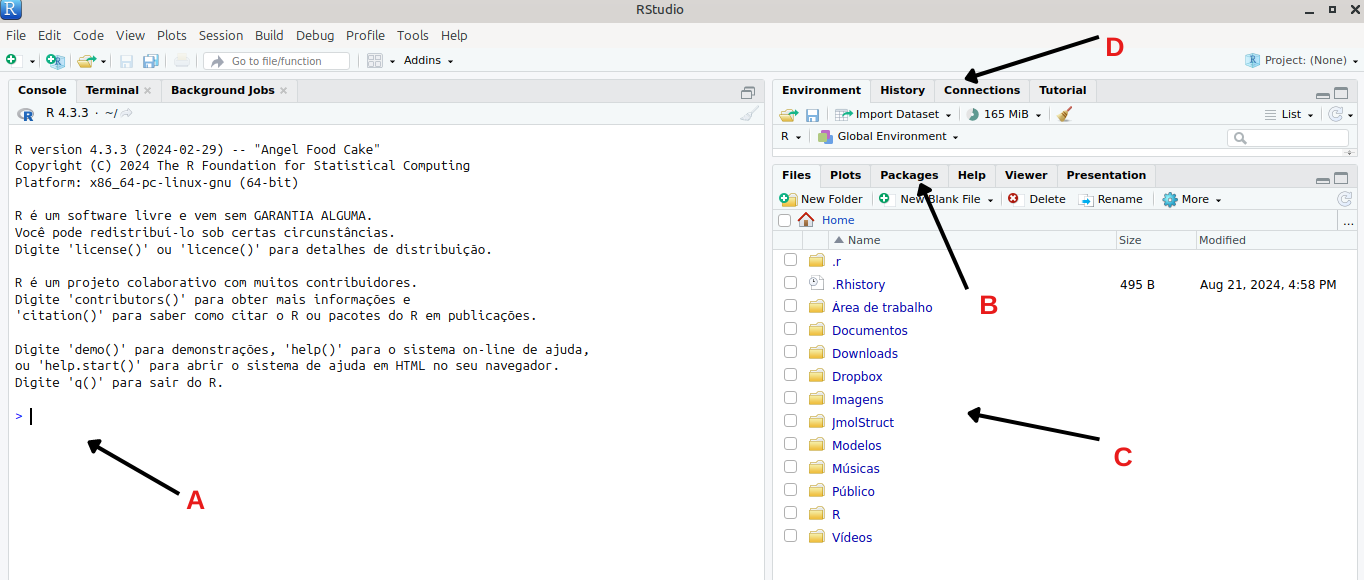
\includegraphics{rstudioWindows2.png}

}

\caption{Janela básica do RStudio. A - área de digitação de comandos
(\emph{prompt}); B - área de abas de trabalho (diretório, gráficos,
pacotes, etc); C - arquivos que aparecem na aba homônima; D - área de
abas de administração (ambiente, história de comandos, etc).}

\end{figure}%

~~~~~~Para nosso trabalho, contudo, será interessante uma área
adicional, a \emph{área de scripts}, a qual se acessa como segue:

\begin{Shaded}
\begin{Highlighting}[]
\NormalTok{File }\SpecialCharTok{{-}}\OtherTok{{-}\textgreater{}}\NormalTok{ New File }\SpecialCharTok{{-}}\OtherTok{{-}\textgreater{}}\NormalTok{ RScript}

\NormalTok{... ou por atalho}\SpecialCharTok{:}\NormalTok{Ctrl }\SpecialCharTok{+}\NormalTok{ Shift }\SpecialCharTok{+}\NormalTok{ N}
\end{Highlighting}
\end{Shaded}

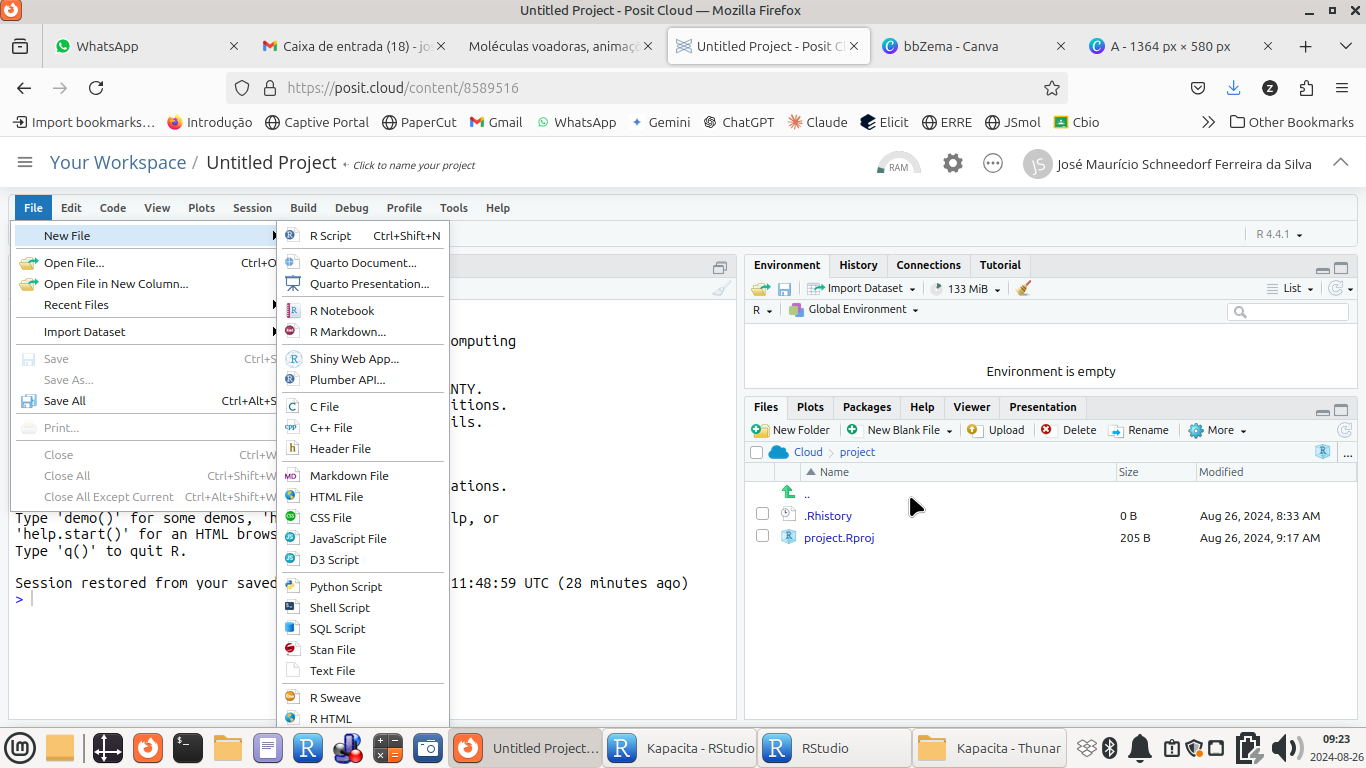
\includegraphics{rstudioScript.png}

~~~~~~Veja que agora a janela principal se divide em quatro partes,
incluindo a aba nova para \emph{scripts}.

\begin{figure}[H]

{\centering 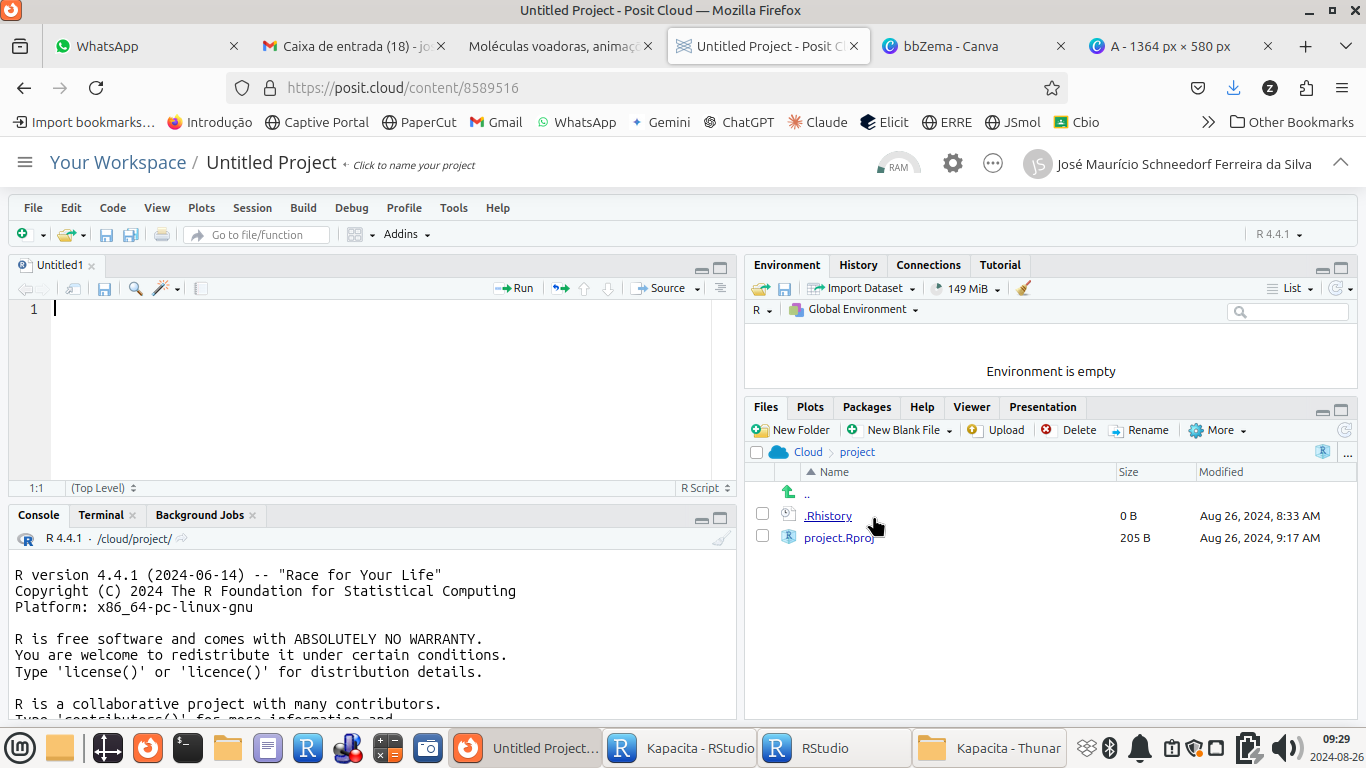
\includegraphics{rstudioScriptAberta.png}

}

\caption{Janela principal do \emph{RStudio} contendo a aba para
elaboração e execução de \emph{scripts}.}

\end{figure}%

\section{\texorpdfstring{Como funcionam os comando no
\texttt{R}}{Como funcionam os comando no R}}\label{como-funcionam-os-comando-no-r}

~~~~~~Todos os comandos do \texttt{R} são compostos por um \emph{nome}
seguido de \emph{argumentos} entre parênteses. \textbf{Não é necessário
a especificação de todos os argumentos}; normalmente bastam de 1 a 3.
Seguem exemplos

\begin{Shaded}
\begin{Highlighting}[]
\FunctionTok{comando}\NormalTok{(argumento }\DecValTok{1}\NormalTok{, argumento }\DecValTok{2}\NormalTok{, argumento }\DecValTok{3}\NormalTok{, ...)}

\NormalTok{Exemplos}\SpecialCharTok{:}
  \FunctionTok{plot}\NormalTok{(x,y)}
  \FunctionTok{mean}\NormalTok{(z)}
  \FunctionTok{read.csv}\NormalTok{(}\AttributeTok{file =} \StringTok{"meus.dados.csv"}\NormalTok{)}
\end{Highlighting}
\end{Shaded}

~~~~~~Para se conhecer os argumentos de um comando, basta você começar a
digitá-lo, tanto na \emph{área de prompt} (canto inferior esquerdo) como
na \emph{área de script}, que o sistema apresenta temporariamente as
opções. Se desejar visualizar essas opções por linha de comando,
contudo, digite função \texttt{args} seguido do comando desejado, como
segue:

\begin{Shaded}
\begin{Highlighting}[]
\FunctionTok{args}\NormalTok{(plot)}
\end{Highlighting}
\end{Shaded}

\section{\texorpdfstring{Elaborando e executando um \emph{script} no
R}{Elaborando e executando um script no R}}\label{elaborando-e-executando-um-script-no-r}

~~~~~~Para se produzir um \emph{script} no \texttt{R}, basta redigir as
linhas de comando de modo similar ao que foi realizado com o
visualizador molecular 3D \emph{Jmol}, ou seja, \emph{separando os
comandos por ponto e vírgula}, ou por linhas individuais, usado a tecla
\emph{Enter} :

\begin{Shaded}
\begin{Highlighting}[]
\NormalTok{x }\OtherTok{=} \DecValTok{5}
\NormalTok{x}\SpecialCharTok{\^{}}\DecValTok{2} \SpecialCharTok{+}\DecValTok{7}
\end{Highlighting}
\end{Shaded}

~~~~~E para executar o \emph{script} acima, basta copiá-lo e colá-lo na
área de \emph{script} aberta. E aí vai uma \textbf{dica de ouro}. Veja
que no canto superior direito do \emph{script} existe um \emph{ícone de
colagem} do texto do \emph{script}. Basta clicar nesse ícone que o texto
estará copiado.

~~~~~~Agora é só colar na aba do \emph{script} aberto (em nuvem, por
exemplo) e executá-lo seguindo-se \emph{alternativamente} as seguintes
ações:

\begin{Shaded}
\begin{Highlighting}[]
\FloatTok{1.}\NormalTok{ Se deseja executar algumas linhas de um }\SpecialCharTok{*}\NormalTok{script}\SpecialCharTok{*}\NormalTok{, pode}\SpecialCharTok{{-}}\NormalTok{se selecionar as linhas e clicar Ctrl }\SpecialCharTok{+}\NormalTok{ Enter ;}

\FloatTok{2.}\NormalTok{ Se desejar executar todo o }\SpecialCharTok{*}\NormalTok{script}\SpecialCharTok{*}\NormalTok{, seleciona}\SpecialCharTok{{-}}\NormalTok{se todo o }\FunctionTok{texto}\NormalTok{ (Ctrl }\SpecialCharTok{+}\NormalTok{ A) seguido da ação acima, Ctrl }\SpecialCharTok{+}\NormalTok{ Enter ;}
\NormalTok{   Opcionalmente, pode}\SpecialCharTok{{-}}\NormalTok{se clicar no ícone }\StringTok{"{-}{-}\textgreater{}Source"}\NormalTok{ ;}
   
\FloatTok{3.}\NormalTok{ Se desejar executar apenas uma linha, basta clicar na linha seguido de Ctrl }\SpecialCharTok{+}\NormalTok{ Enter ;}
\NormalTok{   Opcionalmente, pode}\SpecialCharTok{{-}}\NormalTok{se clicar no ícone }\StringTok{"{-}{-}\textgreater{}Run"}\NormalTok{ ;}
\end{Highlighting}
\end{Shaded}

\section{\texorpdfstring{Algumas recomendações sobre a digitação num
\emph{script} do
\texttt{R}:}{Algumas recomendações sobre a digitação num script do R:}}\label{algumas-recomendauxe7uxf5es-sobre-a-digitauxe7uxe3o-num-script-do-r}

~~~~~~Existem algumas condições básicas pra que um \emph{script} do
\texttt{R} seja lido de forma clara por seu elaborador, bem como
compilado corretamente pelo programa:

\begin{enumerate}
\def\labelenumi{\arabic{enumi}.}
\tightlist
\item
  \emph{Digitação}: sempre que tem um erro no \emph{script} no
  \emph{Rstudio}, surge um sinal em vermelho ao lado esquerdo da linha
  de comando; contornado o erro, o sinal desaparece;
\item
  \emph{Comentários}: para que o \emph{script} seja lido também por
  \emph{``um ser humano''}, é aconselhável tecer comentários nas linhas
  de comando (iniciados por \emph{\#} );
\item
  \emph{Identação}: permita ``identação'' quando a linha estiver um
  pouco longa, clicando na tecla \emph{Enter} após uma separação de
  argumentos por ``vírgula''. Dessa forma, a linha continua logo abaixo,
  mas com um pequeno deslocamento à direita. Isso facilita a
  legibilidade do código.
\item
  \emph{Nomes}: os comandos do \texttt{R} são em língua inglesa. Dessa
  forma, deve-se evitar o uso de variáveis e nomes de arquivos com
  acentuação ou sinais gráficos do Português (ex: \emph{ç}). Além disso,
  o \texttt{R}é um compilador de códigos. Se você definir um nome
  composto para um arquivo ou variável, ou seja, com espaço entre os
  termos (como é normal no cotidiano), o \texttt{R} tentará executar os
  termos separadamente, o que levará em erro. Assim, para nomes de
  variáveis e arquivos, dê preferência a um dos 3 tipos de
  \emph{convenções comuns usadas em programação}, a saber:
\end{enumerate}

\begin{itemize}
\tightlist
\item
  separação por \emph{underline, '' \_ ``} ou hífen; ex:
  minha\_variável, minha-variável
\item
  separação por maiúscula; ex: minhaVariável
\item
  separação por pontos; ex: minha.variável
\end{itemize}

\bookmarksetup{startatroot}

\chapter{Gráficos básicos e
simulações}\label{gruxe1ficos-buxe1sicos-e-simulauxe7uxf5es}

\section{\texorpdfstring{``Plotando'' com o comando \texttt{plot} (meio
óbvio!)}{``Plotando'' com o comando plot (meio óbvio!)}}\label{sec-basico}

~~~~~~Você não precisa instalar mais nada pra trabalhar com gráficos no
\texttt{R}. Isso porque o sistema já possui um conjunto de pacotes na
sua instalação, incluindo um pacote para gráficos (\texttt{graphics}).

~~~~~~Para fazer seu primeiro gráfico, basta \textbf{copiar e colar} o
trecho abaixo num \emph{script} aberto no \emph{Rstudio}, tanto faz se
instalado ou nas nuvens (\emph{RStudio Cloud}), executando-o em seguida.

\begin{Shaded}
\begin{Highlighting}[]
\NormalTok{y }\OtherTok{=} \FunctionTok{c}\NormalTok{(}\DecValTok{1}\NormalTok{,}\DecValTok{2}\NormalTok{,}\DecValTok{4}\NormalTok{,}\DecValTok{8}\NormalTok{,}\DecValTok{16}\NormalTok{,}\DecValTok{32}\NormalTok{)  }\CommentTok{\# vetor de números}
\FunctionTok{plot}\NormalTok{(y)}
\end{Highlighting}
\end{Shaded}

\begin{figure}[H]

{\centering 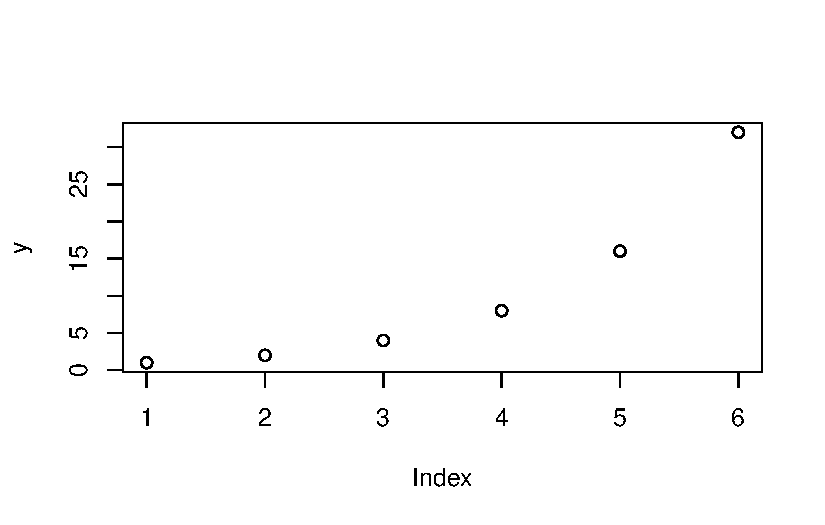
\includegraphics{basico_files/figure-pdf/unnamed-chunk-2-1.pdf}

}

\caption{Um gráfico simples no R.}

\end{figure}%

~~~~~~Se você obteve como resultado a imagem acima, \textbf{parabéns} !!
Você fez o seu primeiro gráfico no \texttt{R} !!! Tá achando pouco ?!
Você fez um gráfico numa \emph{linguagem orientada a objeto em programa
de computação estatística} !!!

~~~~~~Uma \textbf{dica importantíssima\emph{: como se pode observar do
código acima, ``para se colocar valores em sequência, como numa coluna
de planilha eletrônica, o \texttt{R} precisa''ler'' um }vetor* iniciado
por ``c'' (de \emph{concatenated}), seguido dos valores entre parênteses
(\emph{()}) e separados por \emph{vírgula} !}

~~~~~~Agora, se quiser \emph{caprichar um pouco mais}, pode colocar uma
expressão sobre uma sequência de números igualmente espaçados.
Exemplificando:

\begin{Shaded}
\begin{Highlighting}[]
\NormalTok{x }\OtherTok{=} \DecValTok{1}\SpecialCharTok{:}\DecValTok{10} \CommentTok{\# vetor de valores de 0 a 10,  com intervalo unitário}
\NormalTok{y }\OtherTok{=}\NormalTok{ x}\SpecialCharTok{\^{}}\DecValTok{2} \CommentTok{\# expressão aplicada ao vetor "x"}
\FunctionTok{plot}\NormalTok{(x,y) }\CommentTok{\# gráfico produzido}
\end{Highlighting}
\end{Shaded}

\begin{figure}[H]

{\centering 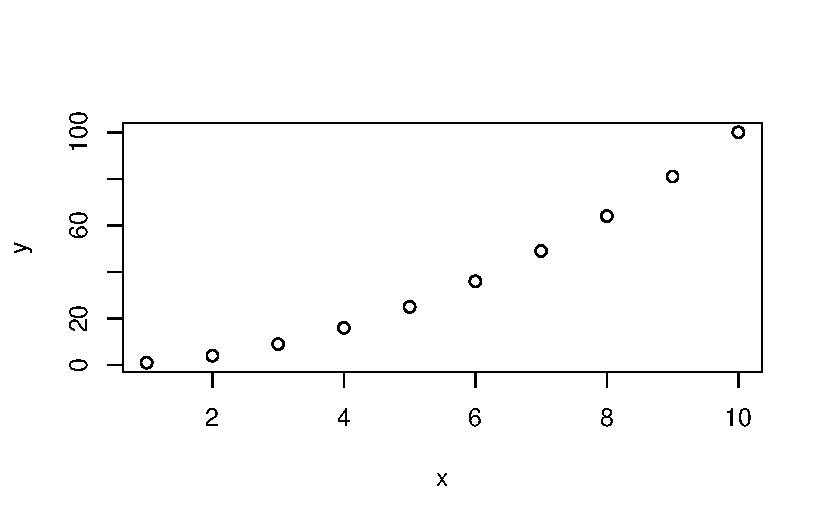
\includegraphics{basico_files/figure-pdf/unnamed-chunk-4-1.pdf}

}

\caption{Um gráfico de relação quadrática (x²) entre \texttt{x}e
\texttt{y}.}

\end{figure}%

~~~~~~Ou\ldots.pode também \emph{escolher os números} que deseja
\emph{plotar}:

\begin{Shaded}
\begin{Highlighting}[]
\NormalTok{x }\OtherTok{=} \FunctionTok{c}\NormalTok{(}\DecValTok{1}\NormalTok{,}\DecValTok{2}\NormalTok{,}\DecValTok{5}\NormalTok{,}\DecValTok{12}\NormalTok{,}\DecValTok{31}\NormalTok{)}
\NormalTok{y}\OtherTok{=} \FunctionTok{c}\NormalTok{(}\DecValTok{4}\NormalTok{,}\SpecialCharTok{{-}}\DecValTok{5}\NormalTok{,}\DecValTok{12}\NormalTok{,}\DecValTok{47}\NormalTok{,}\SpecialCharTok{{-}}\DecValTok{2}\NormalTok{)}
\FunctionTok{plot}\NormalTok{(x,y)}
\end{Highlighting}
\end{Shaded}

\begin{figure}[H]

{\centering 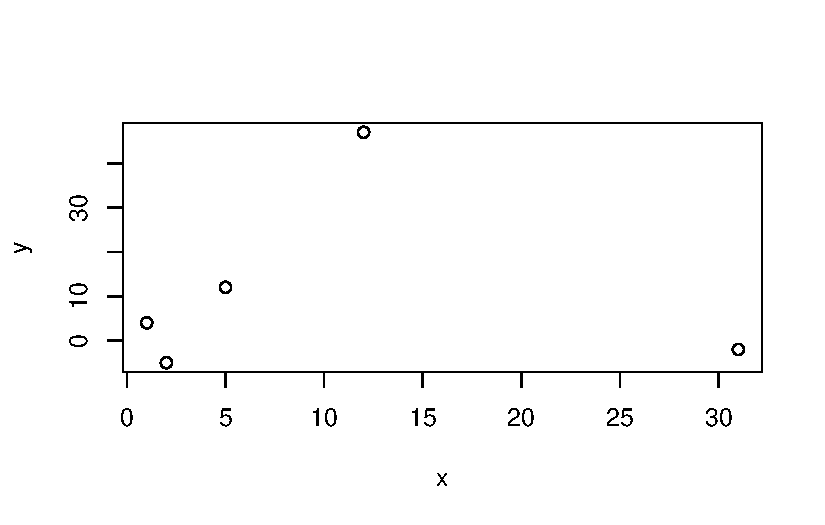
\includegraphics{basico_files/figure-pdf/unnamed-chunk-6-1.pdf}

}

\caption{Gráfico de valores aleatórios de \texttt{x} e \texttt{y}.}

\end{figure}%

\section{Incrementando um pouquinho os
gráficos}\label{incrementando-um-pouquinho-os-gruxe1ficos}

~~~~~~Existe uma quantidade imensa de tutoriais na \emph{web}, além de
uma vasta literatura sobre o uso do pacote \texttt{basic}para se
construir gráficos. Mas a proposta aqui é que você aprenda apenas o
fundamental pra elaborar um gráfico, pois o \emph{objetivo é animá-lo, e
não complicá-lo} !!

~~~~~~Mesmo assim, alguns \emph{argumentos} da função \texttt{plot}
podem ilustrar o potencial de seu uso. Como explicado anteriormente,
ainda que as funções do \texttt{R} possuam diversos argumentos, você
pode executá-la com poucos ou apenas um, somente.

~~~~~~Os argumentos da função \texttt{plot} são os descritos abaixo:

\begin{Shaded}
\begin{Highlighting}[]
\FunctionTok{plot}\NormalTok{(x, }\AttributeTok{y =} \ConstantTok{NULL}\NormalTok{, }\AttributeTok{type =} \StringTok{"p"}\NormalTok{,  }\AttributeTok{xlim =} \ConstantTok{NULL}\NormalTok{, }\AttributeTok{ylim =} \ConstantTok{NULL}\NormalTok{,}
     \AttributeTok{log =} \StringTok{""}\NormalTok{, }\AttributeTok{main =} \ConstantTok{NULL}\NormalTok{, }\AttributeTok{sub =} \ConstantTok{NULL}\NormalTok{, }\AttributeTok{xlab =} \ConstantTok{NULL}\NormalTok{, }\AttributeTok{ylab =} \ConstantTok{NULL}\NormalTok{,}
     \AttributeTok{ann =} \FunctionTok{par}\NormalTok{(}\StringTok{"ann"}\NormalTok{), }\AttributeTok{axes =} \ConstantTok{TRUE}\NormalTok{, }\AttributeTok{frame.plot =}\NormalTok{ axes,}
     \AttributeTok{panel.first =} \ConstantTok{NULL}\NormalTok{, }\AttributeTok{panel.last =} \ConstantTok{NULL}\NormalTok{, }\AttributeTok{asp =} \ConstantTok{NA}\NormalTok{,}
     \AttributeTok{xgap.axis =} \ConstantTok{NA}\NormalTok{, }\AttributeTok{ygap.axis =} \ConstantTok{NA}\NormalTok{,}
\NormalTok{     ...)}
\end{Highlighting}
\end{Shaded}

~~~~~~Um pouco confuso, é ?! Explicando alguns dos argumentos acima, e
outros que funcionam com a função \texttt{plot}:

\begin{Shaded}
\begin{Highlighting}[]
\NormalTok{type }\SpecialCharTok{{-}}\NormalTok{ tipo de plot}\SpecialCharTok{:}\NormalTok{ pontos }\StringTok{"p"}\NormalTok{, linhas }\StringTok{"l"}\NormalTok{, pontos}\SpecialCharTok{+}\NormalTok{linhas com cruzamento }\StringTok{"o"}\NormalTok{, pontos}\SpecialCharTok{+}\NormalTok{linhas sem cruzamento }\StringTok{"b"}\NormalTok{, linhas verticais }\StringTok{"h"}\NormalTok{, steps }\StringTok{"s"}\NormalTok{, sem representação }\StringTok{"n"}\NormalTok{;}

\NormalTok{cex }\SpecialCharTok{{-}}\NormalTok{ tamanho do }\FunctionTok{ponto}\NormalTok{ (ex}\SpecialCharTok{:} \FloatTok{0.5}\NormalTok{, }\DecValTok{20}\NormalTok{);}

\NormalTok{lty }\SpecialCharTok{{-}} \StringTok{"line type"}\NormalTok{, tipo da linha; pode se representado por um }\FunctionTok{valor}\NormalTok{ (}\DecValTok{1}\NormalTok{,}\DecValTok{2}\NormalTok{,...) ou por }\StringTok{"solid"}\NormalTok{, }\StringTok{"dotted"}\NormalTok{, }\StringTok{"dashed"}\NormalTok{, }\StringTok{"dotdash"}\NormalTok{, }\StringTok{"longdash"}\NormalTok{, }\StringTok{"twodash"}\NormalTok{;}

\NormalTok{lwd }\SpecialCharTok{{-}} \StringTok{"line width"}\NormalTok{, largura da }\FunctionTok{linha}\NormalTok{ (}\DecValTok{6}\NormalTok{ níveis)}

\NormalTok{pch }\SpecialCharTok{{-}}\NormalTok{ tipo de }\FunctionTok{ponto}\NormalTok{ (}\DecValTok{1{-}25}\NormalTok{)}

\NormalTok{xlim, ylim }\SpecialCharTok{{-}}\NormalTok{ limite dos eixos; ex}\SpecialCharTok{:}\NormalTok{ ylim}\OtherTok{=}\FunctionTok{c}\NormalTok{(}\SpecialCharTok{{-}}\DecValTok{2}\NormalTok{,}\DecValTok{10}\NormalTok{)}

\NormalTok{xlab, ylab }\SpecialCharTok{{-}} \FunctionTok{etiquetas}\NormalTok{ (}\StringTok{"label"}\NormalTok{) dos gráficos}

\NormalTok{col }\SpecialCharTok{{-}} \FunctionTok{cor}\NormalTok{ (números ou nomes); ex}\SpecialCharTok{:} \StringTok{"red"}\NormalTok{, }\StringTok{"orange"}

\NormalTok{main }\SpecialCharTok{{-}}\NormalTok{ título do gráfico}

\NormalTok{sub }\SpecialCharTok{{-}}\NormalTok{ subtítulo do gráfico}

\NormalTok{log }\SpecialCharTok{{-}}\NormalTok{ eixo logaritmo}
\end{Highlighting}
\end{Shaded}

~~~~~~O gráfico de pontos não é o único que se pode fazer com o pacote
\texttt{graphics}. Também dá pra fazer tudo isso abaixo, com cada função
apresentando os seus próprios argumentos:

\begin{Shaded}
\begin{Highlighting}[]
\FunctionTok{plot}\NormalTok{() }\SpecialCharTok{{-}}\NormalTok{ pontos, linhas, pontos e linhas}
\FunctionTok{barplot}\NormalTok{() }\SpecialCharTok{{-}}\NormalTok{ plot de barras}
\FunctionTok{hist}\NormalTok{() }\SpecialCharTok{{-}}\NormalTok{ histograma}
\FunctionTok{boxplot}\NormalTok{() }\SpecialCharTok{{-}}\NormalTok{ gráfico Box}\SpecialCharTok{{-}}\NormalTok{Whiskers}
\FunctionTok{persp}\NormalTok{() }\SpecialCharTok{{-}}\NormalTok{ gráfico }\DecValTok{3}\NormalTok{D}
\FunctionTok{pie}\NormalTok{() }\SpecialCharTok{{-}}\NormalTok{ gráfico de torta}
\FunctionTok{dotplot}\NormalTok{() }\SpecialCharTok{{-}}\NormalTok{ sequência de }\FunctionTok{valores}\NormalTok{ (com }\SpecialCharTok{*}\NormalTok{jitter}\SpecialCharTok{*}\NormalTok{, espalhameto de pontos)}
\FunctionTok{pairs}\NormalTok{() }\SpecialCharTok{{-}}\NormalTok{ painel múltiplo com todas as variáveis plotadas}
\FunctionTok{matplot}\NormalTok{() }\SpecialCharTok{{-}}\NormalTok{ plota vetores de matrizes, como }\SpecialCharTok{*}\NormalTok{dataframes}\SpecialCharTok{*}
\end{Highlighting}
\end{Shaded}

~~~~~~Mas chega de enrolação !! Para sentir de perto do \emph{``poder''}
desse pacote básico para gráficos, experimente \emph{copiar, colar e
executar} o trecho abaixo:

\section{\texorpdfstring{Simulando curvas com a função
\texttt{curve}}{Simulando curvas com a função curve}}\label{simulando-curvas-com-a-funuxe7uxe3o-curve}

~~~~~~Uma situação bem comum no aprendizado em \emph{Matemática} e de
alguns temas em \emph{Ciências da Natureza} se dá quando desejamos
observar como uma variável se comporta em relação a outra, fornecida uma
equação para tal. Nesse caso, pode-se utilizar a função \texttt{curve}
do \texttt{R}, mais simples até em seus argumentos que a
função\texttt{plot}. Para ilustrar isso, execute separadamente os
exemplos abaixo num \emph{script}:

\begin{Shaded}
\begin{Highlighting}[]
\FunctionTok{curve}\NormalTok{(x}\SpecialCharTok{\^{}}\DecValTok{2}\NormalTok{) }\CommentTok{\# função quadrática}
\FunctionTok{curve}\NormalTok{(}\FunctionTok{log10}\NormalTok{(x), }\AttributeTok{xlim=}\FunctionTok{c}\NormalTok{(}\DecValTok{1}\NormalTok{,}\FloatTok{1e3}\NormalTok{), }\AttributeTok{col=}\StringTok{"blue"}\NormalTok{) }\CommentTok{\# função logarítmica e coloração}
\FunctionTok{curve}\NormalTok{(x}\SpecialCharTok{\^{}}\DecValTok{2{-}2}\SpecialCharTok{*}\NormalTok{x}\SpecialCharTok{+}\DecValTok{7}\NormalTok{, }\AttributeTok{xlim=}\FunctionTok{c}\NormalTok{(}\SpecialCharTok{{-}}\DecValTok{10}\NormalTok{,}\DecValTok{10}\NormalTok{)) }\CommentTok{\# função quadrática com limites no eixo X}
\FunctionTok{curve}\NormalTok{(}\FunctionTok{sin}\NormalTok{(x), }\AttributeTok{from=}\DecValTok{0}\NormalTok{, }\AttributeTok{to=}\DecValTok{90}\NormalTok{, }
      \AttributeTok{xlab=}\StringTok{"ângulo(graus)"}\NormalTok{, }\AttributeTok{ylab=}\StringTok{"seno(ângulo)"}\NormalTok{, }\AttributeTok{col=}\StringTok{"red"}\NormalTok{, }\AttributeTok{n=}\DecValTok{1000}\NormalTok{) }\CommentTok{\# com etiquetas nos eixos}
\end{Highlighting}
\end{Shaded}

\begin{figure}[H]

{\centering 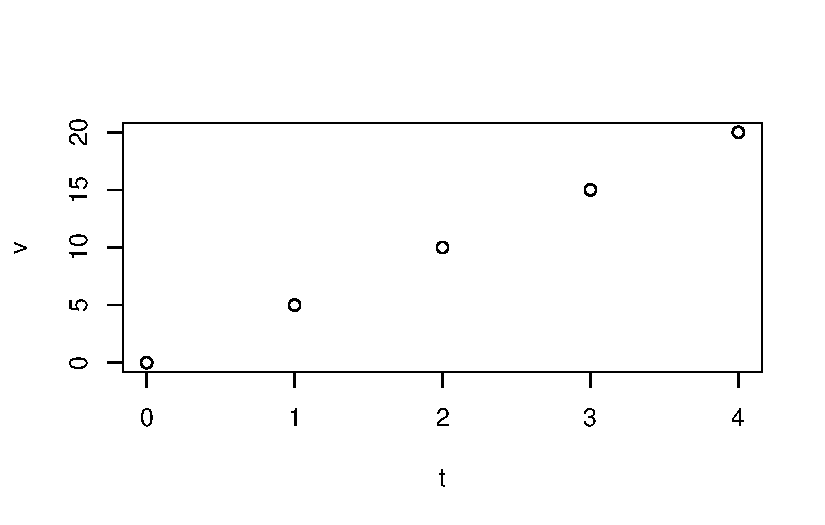
\includegraphics{basico_files/figure-pdf/unnamed-chunk-11-1.pdf}

}

\caption{Alguns exemplos para a função \texttt{curve}.}

\end{figure}%

\bookmarksetup{startatroot}

\chapter{\texorpdfstring{Animando um gráfico básico - o pacote
\texttt{animation.plots}}{Animando um gráfico básico - o pacote animation.plots}}\label{animando-um-gruxe1fico-buxe1sico---o-pacote-animation.plots}

\section{Uma palavrinha antes\ldots{}}\label{uma-palavrinha-antes}

~~~~~~Daqui em diante serão apresentados alguns pacotes do \texttt{R}
que permitem animações, interatividade e simulações gráficas e de
geovisualização. Cada pacote será brevemente descrito, sucedendo-se sua
ilustração com temas contidos no
\href{https://seliga.educacao.mg.gov.br/cardenos-mapa}{MAPA - Material
de Apoio Pedagógico para Aprendizagens} da Secretaria de Educação de
Minas Gerais.

~~~~~~Será fornecida uma breve apresentação de cada \emph{pacote}, o
problema e seu emprego ilustrado junto ao \emph{MAPA}, o trecho de
código para execução/modificação no \emph{RStudio}, seu resultado, e as
vantagens/desvantagens aparentes de cada pacote.

\section{\texorpdfstring{O pacote
\texttt{animation.plots}}{O pacote animation.plots}}\label{o-pacote-animation.plots}

~~~~~~O pacote
\href{https://cran.r-project.org/web/packages/anim.plots/index.html}{animation.plots}
é uma biblioteca para animação de gráficos criados pelo sistema básico
do \texttt{R}, tal como visto na Seção~\ref{sec-basico}.

\bookmarksetup{startatroot}

\chapter{\texorpdfstring{Simulando equações de forma animada - o pacote
\texttt{manipulate}}{Simulando equações de forma animada - o pacote manipulate}}\label{simulando-equauxe7uxf5es-de-forma-animada---o-pacote-manipulate}

\bookmarksetup{startatroot}

\chapter{\texorpdfstring{Comparação de gráficos em Java - o pacote
\texttt{iplots}}{Comparação de gráficos em Java - o pacote iplots}}\label{comparauxe7uxe3o-de-gruxe1ficos-em-java---o-pacote-iplots}

\bookmarksetup{startatroot}

\chapter{Gráficos mais elaborados - pacote
`ggplot2}\label{gruxe1ficos-mais-elaborados---pacote-ggplot2}

\bookmarksetup{startatroot}

\chapter{\texorpdfstring{Animando gráficos do ggplot2 - o pacote
\texttt{gganimate}}{Animando gráficos do ggplot2 - o pacote gganimate}}\label{animando-gruxe1ficos-do-ggplot2---o-pacote-gganimate}

\bookmarksetup{startatroot}

\chapter{\texorpdfstring{Gráficos interativos - o pacote
\texttt{plotly}}{Gráficos interativos - o pacote plotly}}\label{gruxe1ficos-interativos---o-pacote-plotly}

\bookmarksetup{startatroot}

\chapter{\texorpdfstring{Mapas interativos - o pacote
\texttt{leaflet}}{Mapas interativos - o pacote leaflet}}\label{mapas-interativos---o-pacote-leaflet}

\bookmarksetup{startatroot}

\chapter*{References}\label{references}
\addcontentsline{toc}{chapter}{References}

\markboth{References}{References}

\phantomsection\label{refs}
\begin{CSLReferences}{0}{1}
\end{CSLReferences}



\end{document}
